%%%%%%%%%%%%%%%%%%%%%%%%%%%%%%%%%%%%%%%%%
% Masters/Doctoral Thesis 
% LaTeX Template
% Version 2.5 (27/8/17)
%
% This template was downloaded from:
% http://www.LaTeXTemplates.com
%
% Version 2.x major modifications by:
% Vel (vel@latextemplates.com)
%
% This template is based on a template by:
% Steve Gunn (http://users.ecs.soton.ac.uk/srg/softwaretools/document/templates/)
% Sunil Patel (http://www.sunilpatel.co.uk/thesis-template/)
%
% Template license:
% CC BY-NC-SA 3.0 (http://creativecommons.org/licenses/by-nc-sa/3.0/)
%
%%%%%%%%%%%%%%%%%%%%%%%%%%%%%%%%%%%%%%%%%
%La plantilla base fue utilizada y modificada por Fernando Salazar y Rolando Sotelo
%----------------------------------------------------------------------------------------
%	PACKAGES AND OTHER DOCUMENT CONFIGURATIONS
%----------------------------------------------------------------------------------------

\documentclass[
	12pt, % The default document font size, options: 10pt, 11pt, 12pt
	%oneside, % Two side (alternating margins) for binding by default, uncomment to switch to one side
	spanish, % ngerman for German
	es-tabla,
	singlespacing, % Single line spacing, alternatives: onehalfspacing or doublespacing
	%draft, % Uncomment to enable draft mode (no pictures, no links, overfull hboxes indicated)
	%nolistspacing, % If the document is onehalfspacing or doublespacing, uncomment this to set spacing in lists to single
	%liststotoc, % Uncomment to add the list of figures/tables/etc to the table of contents
	%toctotoc, % Uncomment to add the main table of contents to the table of contents
	%parskip, % Uncomment to add space between paragraphs
	%nohyperref, % Uncomment to not load the hyperref package
	headsepline, % Uncomment to get a line under the header
	%chapterinoneline, % Uncomment to place the chapter title next to the number on one line
	%consistentlayout, % Uncomment to change the layout of the declaration, abstract and acknowledgements pages to match the default layout
	]{MastersDoctoralThesis} % The class file specifying the document structure
	
% Paquetes:
\usepackage[utf8]{inputenc} % Required for inputting international characters
\usepackage[T1]{fontenc} % Output font encoding for international characters
\usepackage{mathpazo} % Use the Palatino font by default
\usepackage[backend=biber,style=ieee,natbib=true]{biblatex} % Para Formato IEEE
\addbibresource{Referencias.bib} % The filename of the bibliography
\usepackage[autostyle=true]{csquotes} % Required to generate language-dependent quotes in the bibliography
\usepackage{xcolor}
\usepackage{lscape} %Para poner páginas horizontales
\usepackage{booktabs}
\usepackage{multirow}
\usepackage{rotating}
\usepackage{algorithm}
\usepackage[T1]{fontenc} % Codificación de fuente
\usepackage{lmodern} % Fuente compatible
\usepackage[noend]{algpseudocode}%Para incluir algoritmos
\usepackage{amssymb}
\usepackage{amsmath}
\renewcommand{\spanishtablename}{Tabla}
\renewcommand{\spanishlisttablename}{Índice de tablas}
%\renewcommand{\acknowledgmentsname}{Agradecimientos}
%\addto\captionsspanish{\renewcommand{\acknowledgmentsname}{Agrade}}
\newcommand\myworries[1]{\textcolor{red}{#1}} %Para incorporar TODOs en el documento (en color rojo)
\setlength\parindent{0pt} %Para evitar la sangría default que implementa la clase

%----------------------------------------------------------------------------------------
%	MARGIN SETTINGS
%----------------------------------------------------------------------------------------

\geometry{
	paper=letterpaper, % Change to letterpaper for US letter
	inner=2cm, % Inner margin
	outer=2cm, % Outer margin
	bindingoffset=.5cm, % Binding offset
	top=1.5cm, % Top margin
	bottom=1.5cm, % Bottom margin
	%showframe, % Uncomment to show how the type block is set on the page
}

%----------------------------------------------------------------------------------------
%	THESIS INFORMATION
%----------------------------------------------------------------------------------------

\thesistitle{SIMULADOR DE MODELOS DE TRÁFICO PARA NODOS IOT EN UNA RED CELULAR DE 5G} % Your thesis title, this is used in the title and abstract, print it elsewhere with \ttitle
%\supervisor{} % Your supervisor's name, this is used in the title page, print it elsewhere with \supname
%\examiner{} % Your examiner's name, this is not currently used anywhere in the template, print it elsewhere with \examname
\degree{Ingeniería en Telemática} % Your degree name, this is used in the title page and abstract, print it elsewhere with \degreename
\author{} % Your name, this is used in the title page and abstract, print it elsewhere with \authorname 
\addresses{} % Your address, this is not currently used anywhere in the template, print it elsewhere with \addressname

\subject{Comunicaciones Móviles} % Your subject area, this is not currently used anywhere in the template, print it elsewhere with \subjectname
\keywords{mMTC, NB-IoT, PD-NOMA, 5G, simulador de eventos discretos, QoS.} % Keywords for your thesis, this is not currently used anywhere in the template, print it elsewhere with \keywordnames
\university{\href{https://www.upiita.ipn.mx/}{Unidad Profesional interdisciplinaria de Ingeniería y Tecnologías Avanzadas}} % Your university's name and URL, this is used in the title page and abstract, print it elsewhere with \univname
\department{\href{}{}} % Your department's name and URL, this is used in the title page and abstract, print it elsewhere with \deptname
\group{\href{}{}} % Your research group's name and URL, this is used in the title page, print it elsewhere with \groupname
\faculty{\href{}{}} % Your faculty's name and URL, this is used in the title page and abstract, print it elsewhere with \facname

\AtBeginDocument{
\hypersetup{pdftitle=\ttitle} % Set the PDF's title to your title
%\hypersetup{pdfauthor=\authorname} % Set the PDF's author to your name
\hypersetup{pdfkeywords=\keywordnames} % Set the PDF's keywords to your keywords
}

\begin{document}
%\bibliographystyle{IEEEtran}
\frontmatter % Use roman page numbering style (i, ii, iii, iv...) for the pre-content pages

\pagestyle{plain} % Default to the plain heading style until the thesis style is called for the body content

%----------------------------------------------------------------------------------------
%	TITLE PAGE
%----------------------------------------------------------------------------------------

\begin{titlepage}
\begin{center}

%\vspace*{.06\textheight}
{\scshape\LARGE \univname\par}\vspace{1cm} % University name

\includegraphics[scale=.8]{LogoUPIITA}\\ % University/department logo - uncomment to place it
\vspace*{.03\textheight}
\textsc{\Large Proyecto Terminal II}\\[0.7cm] % Thesis type

\HRule \\[0.4cm] % Horizontal line
{\huge \bfseries \ttitle\par}\vspace{0.4cm} % Thesis title
\HRule \\[0.4cm] % Horizontal line

\begin{minipage}[t]{0.4\textwidth}
\begin{flushleft} \large
\emph{Autores:}\\
Rolando \textsc{Sotelo Alarcon} \newline
Luis Fernando \textsc{Salazar Ordoñez} \newline
\end{flushleft}
\end{minipage}
\begin{minipage}[t]{0.4\textwidth}
\begin{flushright} \large
\emph{Asesores:} \\
Dr. Domingo \textsc{Lara Rodriguez} \newline
Dr. Noe \textsc{Torres Cruz}
\end{flushright}
\end{minipage}\\[.6cm]
 
\vfill

\large \textit{Una tesis presentada en cumplimiento de los requisitos \\para el grado de \degreename}\\[0.2cm] % University requirement text
%\textit{in the}\\[0.4cm]
%\groupname\\\deptname\\[2cm] % Research group name and department name
 
\vfill

{\large Julio 2020}\\[4cm] % Date
 
\vfill
\end{center}
\end{titlepage}

%----------------------------------------------------------------------------------------
%	DECLARATION PAGE
%----------------------------------------------------------------------------------------

%\begin{declaration}
%\addchaptertocentry{\authorshipname} % Add the declaration to the table of contents
%\noindent I, \authorname, declare that this thesis titled, \enquote{\ttitle} and the work presented in it are my own. I confirm that:

%\begin{itemize} 
%\item This work was done wholly or mainly while in candidature for a research degree at this University.
%\item Where any part of this thesis has previously been submitted for a degree or any other qualification at this University or any other institution, this has been clearly stated.
%\item Where I have consulted the published work of others, this is always clearly attributed.
%\item Where I have quoted from the work of others, the source is always given. With the exception of such quotations, this thesis is entirely my own work.
%\item I have acknowledged all main sources of help.
%\item Where the thesis is based on work done by myself jointly with others, I have made clear exactly what was done by others and what I have contributed myself.\\
%\end{itemize}
 
%\noindent Signed:\\
%\rule[0.5em]{25em}{0.5pt} % This prints a line for the signature
 
%\noindent Date:\\
%\rule[0.5em]{25em}{0.5pt} % This prints a line to write the date
%\end{declaration}

%\cleardoublepage

%----------------------------------------------------------------------------------------
%	QUOTATION PAGE
%----------------------------------------------------------------------------------------

%\vspace*{0.2\textheight}

%\noindent\enquote{\itshape Thanks to my solid academic training, today I can write hundreds of words on virtually any topic without possessing a shred of information, which is how I got a good job in journalism.}\bigbreak

%\hfill Dave Barry

%----------------------------------------------------------------------------------------
%	ABSTRACT PAGE
%----------------------------------------------------------------------------------------

\begin{abstract}
\addchaptertocentry{\abstractname} % Add the abstract to the table of contents
Resumen:
En este documento se presenta el desarrollo de un simulador a nivel de sistema, programado bajo el paradigma de eventos discretos, que permite modelar el servicio que la red de comunicación celular de quinta generación (5G), ofrece a nodos de Internet de las cosas (IoT). El simulador se enfocó en el caso de uso mIoT, el cual comprende principalmente de nodos IoT estáticos de baja complejidad que además se encuentran en gran cantidad dentro de los escenarios de esta red. La arquitectura del simulador contempló cuatro módulos clave para su ejecución: un modelo de despliegue de UEs, un modelo de canal, un esquema de acceso múltiple al medio no ortogonal y modelos de tráfico adecuados para modelar distintos servicios. Asimismo, se consideró el fundamentar la fiabilidad de los resultados obtenidos por el simulador mediante la previa prueba e implementación de modelos de tráfico ya estudiados en la literatura concerniente al desempeño de sistemas celulares. Con los resultados del simulador se determinaron qué configuraciones y parámetros iniciales de la arquitectura de red propuesta satisfacen una óptima calidad de servicio (QoS) para el caso de uso mIoT.\newline \\
Palabras clave: \keywordnames\\ 
\textit{Abstract: }\\ 
\textit{Keywords: \keywordnames}\\

\myworries{TODO: Realizar la actualización del abstract y agregar su traducción al ingles}
\end{abstract}

%----------------------------------------------------------------------------------------
%	ACKNOWLEDGEMENTS
%----------------------------------------------------------------------------------------

\begin{acknowledgements}
\addchaptertocentry{\acknowledgementname} % Add the acknowledgements to the table of contents
Agradecimientos\ldots
\end{acknowledgements}

%----------------------------------------------------------------------------------------
%	LIST OF CONTENTS/FIGURES/TABLES PAGES
%----------------------------------------------------------------------------------------

\tableofcontents % Prints the main table of contents

\listoffigures % Prints the list of figures

\listoftables % Prints the list of tables

%----------------------------------------------------------------------------------------
%	ABBREVIATIONS
%----------------------------------------------------------------------------------------
\begin{abbreviations}{ll} % Include a list of abbreviations (a table of two columns)
\textbf{3GPP} & \textbf{3}rd \textbf{G}eneration \textbf{P}artnership \textbf{P}roject\\%Ejemplo de acrónimo correcto
\textbf{4G} & Cuarta generación de Comunicaciones Móviles\\
\textbf{5G NR} & 5G New Radio\\
\textbf{ARIB} &	Association of Radio Industries and Businesses\\
\textbf{ARPU} &	Average Revenue Per User\\
\textbf{ATIS} & Alliance for Telecommunications Industry Solutions\\
\textbf{AWGN} &	Additive White Gussian Noise\\
\textbf{apd} & Average Power Decay (a.k.a. PLE)\\
\textbf{BS} & Base Station\\
\textbf{BSs} & Base Stations\\
\textbf{BW} & Bandwidth\\
\textbf{CCSA} &	China Communications Standars Associations\\
\textbf{CD-NOMA} & Code Division NOMA\\
\textbf{CIoT} & Cellular IoT\\
\textbf{CMMPP} & Coupled Markov Modulated Poisson Process\\
\textbf{CT} & Central Terminal\\
\textbf{DES} & Discrete Event Simulation\\
\textbf{DL} & DownLink\\
\textbf{ED} & Event-Driven\\
\textbf{EIRP} & Efective Isotropic Radiated Power\\
\textbf{eMBB} &	Enhanced Mobile Broadband\\
\textbf{eMTC} &	Enhanced Machine Type Communications\\
\textbf{ETSI} &	European Telecommunications Standars institute\\
\textbf{EUTRA} & Evolved UMTS Terrestrial Radio Access\\
\textbf{fc} & Frecuencia Portadora\\
\textbf{GIL} & Global Interpreter Lock\\
\textbf{HPPP} & Homogeneous Poisson Point Process\\
\textbf{HTC} & Human Type Communication\\
\textbf{IEEE} &	Institute of Electrical and Electronics Engineers\\
\textbf{IFT} & Instituto Federal de Telecomunicaciones\\
\textbf{InH} & Indoor Hotspot\\
\textbf{IoT} & Internet of Things\\
\textbf{ITU} & International Telecommunication Union\\
\textbf{ITU-R} & ITU Radiocommunications\\
\textbf{KPI} & Key Performance Indicator\\
\textbf{KPIs} &	Key Performance Indicators\\
\textbf{LoS} & Line of Sight\\
\textbf{LPWAN} & Low Power Wide Area Networks\\
\textbf{LSP} & Large-Scale Parameters\\
\textbf{LTE} & Long Term Evolution\\
\textbf{LTE-M} & LTE-MTC\\
\textbf{M2M} & Machine to Machine\\
\textbf{MA} & Multiple Access\\
\textbf{MAC} & Media Access Control\\
\textbf{MIMO} &	Multiple Inputs Multiple Outputs\\
\textbf{mIoT} &	Massive IoT\\
\textbf{MMPP} &	Markov Modulated Poisson Process\\
\textbf{mMTC} &	Massive Machine Type Communications\\
\textbf{MS} & Mobile Station\\
\textbf{MT} & Mobile Terminal\\
\textbf{MTC} & Machine Type Communication\\
\textbf{MTs} & Mobile Terminals\\
\textbf{M2M} &Machine to machine\\
\textbf{NB-IoT} & Narrow-Band Internet of Things\\
\textbf{NGMN} &	Next Generation Mobile Networks\\
\textbf{NLoS} &	Non-Line of Sight\\
\textbf{NOMA} &	Non-Orthogonal Multiple Access\\
\textbf{OFDMA} & Orthogonal Frequency Division Multiple Access\\
\textbf{OMA} & Orthogonal Multiple Access\\
\textbf{PD-NOMA} & Power Division NOMA\\
\textbf{PE} & Payload Exchange\\
\textbf{PL} & Path Loss\\
\textbf{PLE} & Path Loss Exponent\\
\textbf{PPP} & Poisson Point Process\\
\textbf{PRB} & Physical Resource Block\\
\textbf{PSM} & Power Saving Mode\\
\textbf{PU} & Periodic Update\\
\textbf{QoS} & Quality of Service\\
\textbf{RAN} & Radio Access Networks\\
\textbf{RF} & Radio Frequency\\
\textbf{RFID} & Radio Frequency Identification\\
\textbf{Rx} & Receiver\\
\textbf{SA} & Stand-alone\\
\textbf{SA 2} & System Aspects\\
\textbf{SC-FDMA} & Single Carrier Frequency Division Multiple Access\\
\textbf{SF} & Shadow Fading\\
\textbf{SIC} & Successive Interference Cancelation\\
\textbf{SINR} & Signal to Interference plus Noise Ratio\\
\textbf{SISO} & Single Input Single Output\\
\textbf{SM} & Suburban Macro\\
\textbf{SMM} & Semi-Markov Model\\
\textbf{TDD} & Time Division Duplexing\\
\textbf{TDMA} &	Time Division Multiple Access\\
\textbf{TR} & Technical Report\\
\textbf{TSDO} &	Telecommunications Standards Development Organization\\
\textbf{TSDOs} & Telecommunications Standards Development Organizations\\
\textbf{TSDSI} & Telecommunications Standards Development Society, India\\
\textbf{TSG} & Technical Specifications Group\\
\textbf{TTA} & Telecommunications Technology Association of Korea\\
\textbf{TTC} & Telecommunication Technology Committee\\
\textbf{Tx} & Transmitter\\
\textbf{UE} & User Equipment\\
\textbf{UL} & UpLink\\
\textbf{UMa} & Urban Macro\\
\textbf{UMi} & Urban Micro\\
\textbf{UMTS} &	Universal Mobile Telecommunications System\\
\textbf{URLLC} & Ultra-Reliable and Low-Latency Communications\\
\end{abbreviations}

%----------------------------------------------------------------------------------------
%	PHYSICAL CONSTANTS/OTHER DEFINITIONS
%----------------------------------------------------------------------------------------

%\begin{constants}{lr@{${}={}$}l} % The list of physical constants is a three column table

% The \SI{}{} command is provided by the siunitx package, see its documentation for instructions on how to use it

%Speed of Light & $c_{0}$ & \SI{2.99792458e8}{\meter\per\second} (exact)\\
%Constant Name & $Symbol$ & $Constant Value$ with units\\

%\end{constants}

%----------------------------------------------------------------------------------------
%	SYMBOLS
%----------------------------------------------------------------------------------------

%\begin{symbols}{lll} % Include a list of Symbols (a three column table)
%\myworries{TODO: Agregar simbolos}
%$a$ & distance & \si{\meter} \\
%$P$ & power & \si{\watt} (\si{\joule\per\second}) \\
%Symbol & Name & Unit \\

%\addlinespace % Gap to separate the Roman symbols from the Greek

%$\omega$ & angular frequency & \si{\radian} \\

%\end{symbols}

%----------------------------------------------------------------------------------------
%	DEDICATION
%----------------------------------------------------------------------------------------

\dedicatory{For/Dedicated to/To my \ldots} 

%----------------------------------------------------------------------------------------
%	THESIS CONTENT - CHAPTERS
%----------------------------------------------------------------------------------------

\mainmatter % Begin numeric (1,2,3...) page numbering

\pagestyle{thesis} % Return the page headers back to the "thesis" style

% Include the chapters of the thesis as separate files from the Chapters folder
% Uncomment the lines as you write the chapters

% Chapter 1

\chapter{Presentación del Proyecto} % Main chapter title

\label{Chapter1} % Change X to a consecutive number; for referencing this chapter elsewhere, use \ref{ChapterX}

%----------------------------------------------------------------------------------------

% Define some commands to keep the formatting separated from the content 
\newcommand{\keyword}[1]{\textbf{#1}}
\newcommand{\tabhead}[1]{\textbf{#1}}
\newcommand{\code}[1]{\texttt{#1}}
\newcommand{\file}[1]{\texttt{\bfseries#1}}
\newcommand{\option}[1]{\texttt{\itshape#1}}

%----------------------------------------------------------------------------------------
%	SECTION 1
%----------------------------------------------------------------------------------------

\section{INTRODUCCIÓN}

Imaginar nuestra vida sin los beneficios brindados por los sistemas de comunicación de hoy en día, o tan sólo sin la tecnología presente en este ámbito desde los últimos 20 años es ya muy difícil, y esto se debe a que en el presente una gran parte de las tareas y actividades, muchas de ellas cruciales para el funcionamiento de nuestras sociedades, operan eficientemente sí y sólo sí se está propiamente conectado y en facultades de compartir información \parencite{Fettweis2014}.\newline

Los sistemas de comunicación celular han tenido saltos generacionales desde la conocida como primera generación, la cual saldría al mercado a finales de la década de los 70’s e inicio de los 80’s, hasta el presente con el desarrollo de la próxima generación (5G), la cual comenzará su implementación en el año 2020. En \parencite{Fettweis2014} encontramos que:\newline

\hspace*{10mm} {“La primera y segunda generación de comunicaciones móviles estuvieron dominadas por señales analógicas de audio y posteriormente señales digitales de audio y texto. La tercera generación se trató más de escalar el número de usuarios en la red […] pero fue abrumada por un tsunami de contenido de imágenes y videos.”}\newline

\myworries{TODO: poner esta parte en sangría}\newline

Cada uno de estos saltos de generación ha estado motivado por distintos requerimientos de servicio, necesidades de los usuarios y la aparición de nuevas tecnologías que han buscado ser una vía para facilitar la comunicación entre individuos de todo el mundo y ahora, más recientemente, la comunicación entre máquinas.\newline

El aumento de la tasa de transmisión de datos ha sido siempre un factor a tener en cuenta para el desarrollo de los estándares de las nuevas generaciones de redes móviles, por ejemplo, para la nueva generación se espera “un pico de transmisión de al menos 1 Gb/s al tiempo de su introducción en 2020, esperando que crezca hasta los 10Gb/s para 2025”, \parencite{Fettweis2016}. Pero el sistema de comunicaciones móviles de quinta generación ha estado, además de eso, motivado por un mayor volumen de transmisión de datos, un incremento radical en la cantidad de dispositivos conectados a la red, una menor latencia y una mayor duración de batería para los dispositivos de bajo consumo.\newline

Las limitaciones presentes hasta ahora para las comunicaciones IoT celulares, se deben principalmente a que la red de comunicación móvil fue creada para voz y aplicaciones de texto, evolucionando eventualmente a una transmisión de archivos como imágenes y videos predominante en el enlace de bajada. Por otro lado la comunicación de dispositivos IoT tiene un conjunto de requerimientos muy distintos. Pero es ahora con la quinta generación que se promete brindar las herramientas que esta tecnología necesita para alcanzar su máximo potencial. 5G se trata entonces de la propuesta de crear una red de comunicaciones que logre implementar tanto los servicios inherentes a las necesidades de comunicación entre los humanos y aquellas necesidades de comunicación entre las máquinas. El cumplir con estas últimas necesidades, aseguraría brindar una calidad de servicio óptima para la nueva ola de dispositivos de IoT que se espera estén ya conectados a la red para 2020.\newline

Este proyecto presenta el diseño de un simulador de eventos discretos, el cual modeló el servicio prestado por la arquitectura de red celular que aquí se propone a nodos IoT. Su arquitectura contempló la próxima generación móvil a implementarse (5G) y los servicios seleccionados para atender a aplicaciones del caso de uso mIoT. Este simulador se enfocó en el tráfico generado por dispositivos NB-IoT y con los resultados obtenidos se esclareció sobre qué configuraciones de red son ideales para conseguir una óptima calidad de servicio.\newline

%----------------------------------------------------------------------------------------
%	SECTION 2
%----------------------------------------------------------------------------------------

\section{PLANTEAMIENTO DEL PROBLEMA}

En los recientes años se ha estado presenciando la definición de la tecnología de comunicación móvil 5G en estándares, para su posterior introducción a partir de 2020, y como se resalta en \parencite{Fettweis2016} la nueva generación no sólo seguirá la línea de incrementar la velocidad de transmisión como se ha venido haciendo en cada salto generacional, sino que también traerá consigo la posibilidad de una conectividad adicional sin precedentes, todo esto motivado por la cantidad masiva de dispositivos de IoT que se esperan. Según Ericsson Mobility Report \parencite{Ericsson2019}, 22.3 mil millones de dispositivos en el 2024, pertenecerán a una aplicación de IoT. De manera que 5G dará servicio a una enorme cantidad de dispositivos IoT, cada dispositivo enviará pequeños paquetes de datos a lo largo de mucho tiempo, además de que existirá una cierta sincronía en el tráfico generado. Lo anterior ha provocado el desarrollo de nuevas tecnologías que proponen distintas formas de agrupamiento de estos nodos, distintas formas de acceder a los recursos, distintas propuestas de comunicación entre ellos y nuevas formas de que ahorren energía. Siempre teniendo en cuenta los KPIs de la red, como dar servicio a una cantidad masiva de nodos, la duración de la batería de estos y la menor latencia en comunicaciones críticas \footnote{\ Comunicaciones\ que\ requieren\ de\ una\ urgente\ respuesta\ debido\ a\ su\ naturaleza,\ por\ ejemplo\ los\ coches\ auto-dirigidos.} , como se menciona en \parencite{NGMN}.\newline

Esto ha resultado en nuevos retos para la implementación de la red, para la cual se desarrolla tecnología o se mejora la ya existente. En \parencite{GSMAssociation2019}, se presenta la tecnología NB-IoT (Narrow-Band IoT), originalmente creada como una solución que brindara servicio a nodos IoT en LTE. Esta tecnología formará parte de los estándares de 5G, como 3GPP\footnote{\ $  $The\ 3rd\ Generation\ Partnership\ Project\ (3GPP),\ desarrolladores\ del\ est\textrm{\'{a}}ndar\ NB-IoT\ y\ el\ 5G\ NR}
lo ha indicado a la ITU (International Telecommunication Union). Se pretende que con esta tecnología y algunas mejoras, la red 5G sea capaz de brindar servicio a aplicaciones del caso de uso mMTC\footnote{Cabe mencionar que los casos de uso o tecnologías mIoT y mMTC son análogas.}, para el cual se esperan tener decenas de miles de dispositivos conectados por celda. \newline

En el futuro, los escenarios de IoT, tendrán una enorme cantidad de dispositivos conectados en comparación con los actuales escenarios de la red 4G \parencite{Whatis5G}. Por lo tanto, las tecnologías de 5G deberán brindar servicio a muchos dispositivos usando recursos limitados. Pero dada la elevada complejidad con la que el modelo de un sistema de comunicación como la red 5G puede contar, si de éste se quieren obtener resultados útiles, resulta casi imposible el analizar su comportamiento sino a través de una simulación.\newline

Los patrones de tráfico de nodos de IoT varían según su caso de uso, los cuales se dividen normalmente en tres: eMBB, uRLLC y mMTC. Para mMTC también llamado mIoT, en el cual se enfocará el proyecto, se tienen nodos en su amplia mayoría estáticos y como se ve en \parencite{IoTTrafficHossfeld}, para estos nodos podemos considerar por los menos dos patrones de tráfico: el periódico, y el aleatorio ,de manera que el modelo de tráfico deberá tener en consideración esto. Como se puede apreciar en \parencite{IoTTrafficHossfeld}, un problema crítico del Internet de las cosas masivo (mIoT) en las redes móviles es que los dispositivos de IoT causarán una gran congestión en esta si es que no se incorporan mejoras en las arquitecturas de estas redes. Este problema se ve acrecentado debido a que el tráfico de los nodos mIoT presenta cierta sincronía espacial y temporal dependiendo de la aplicación a la que pertenezcan.\newline

Por lo anterior, para la red 5G se necesitan realizar simulaciones en sus distintos casos de uso, que generen resultados sobre qué arquitectura de red y tecnologías brindan un resultado óptimo. Con la realización de este proyecto se pretende aportar al campo de las comunicaciones móviles de quinta generación, que está específicamente interesado en el servicio prestado a los nodos de IoT, de una herramienta de simulación que genere resultados que permitan realizar comparaciones entre distintas configuraciones de red. Todo esto con el fin de que la red 5G próxima a ser desplegada, cumpla con una óptima calidad de servicio para el caso de uso mIoT.\newline

%----------------------------------------------------------------------------------------
%	SECTION 3
%----------------------------------------------------------------------------------------

\section{OBJETIVOS}
\subsection{OBJETIVO GENERAL}

Diseñar e implementar un simulador de teletráfico para el ambiente de Internet de las cosas masivo (mIoT) en una red celular de quinta generación (5G), por medio de la programación de eventos discretos, con la finalidad de evaluar el desempeño de esta red en términos de la cantidad de recursos requeridos para satisfacer niveles esperados de calidad de servicio (QoS).\newline

\subsection{OBJETIVOS ESPECÍFICOS}

\begin{itemize}
    \item Determinar el escenario a implementar, mediante el análisis de requerimientos, para definir después los parámetros de entrada en el modelado del simulador.
    \item Seleccionar los modelos (despliegue, propagación, técnica de acceso múltiple) aplicables a una simulación a nivel de sistema para la comunicación entre nodos IoT y la red 5G.
    \item Seleccionar y determinar los modelos de tráfico a analizar para nodos IoT que hayan sido propuestos en la red 5G, mediante la lectura de distintas publicaciones en revistas científicas, para simular el modelo más adecuado según los alcances propuestos.
    \item Determinar los parámetros de desempeño de la red (KPIs), mediante el análisis de distintas publicaciones científicas, con la finalidad de establecer métricas de QoS.
    \item Definir el procedimiento de la simulación mediante la especificación de su arquitectura y elaboración de diagramas de su funcionamiento y procesos, con el fin de integrar una metodología para su implementación.
    \item Implementar los modelos y protocolos que definen a la comunicación entre los nodos IoT y la red 5G, mediante algoritmos computacionales (incluyendo la técnica de eventos discretos) y de acuerdo a la arquitectura previamente definida.
    \item Implementar una técnica de paralelismo, mediante el uso de multiprocesamiento, con la finalidad de reducir los tiempos de ejecución de las simulaciones.
    \item Evaluar y analizar cada modelo analítico con el uso de escenarios de pruebas y calibración para poder realizar comparaciones con los resultados teóricos esperados y verificar la fiabilidad del simulador 
    \item Simular el modelo de sistema propuesto, mediante la variación de los parámetros de entrada, para caracterizar el desempeño del sistema en términos del tráfico que se puede ofrecer y la cantidad de recursos requeridos para satisfacer objetivos de QoS.
\end{itemize}

%----------------------------------------------------------------------------------------
%	SECTION 4
%----------------------------------------------------------------------------------------

\section{JUSTIFICACIÓN}

En la gran mayoría de los trabajos de investigación revisados, se han realizado estudios de rendimiento de los sistemas de comunicación móvil de quinta generación. Estos se concentran en evaluar distintos modelos, frecuentemente se considera, un modelo de distribución de BSs y UEs, uno de canal, y un esquema de acceso multiple, sin embargo no hay mucha investigación acerca de incorporar todos estos componentes en conjunto con modelos de tráfico para el caso específico de mIoT. La aportación que se pretende hacer con este proyecto se encuentra precisamente en ese ámbito.\newline

Los enlaces de comunicación inalámbrica experimentan fenómenos físicos perjudiciales al canal como lo son las multi-trayectorias y los desvanecimientos debido a grandes objetos que se interceptan en la trayectoria de la propagación, además el rendimiento de los sistemas celulares inalámbricos tiende a limitarse debido a la interferencia de otros usuarios. Estas condiciones complejas del canal son difíciles de describir con un simple modelo analítico, es por esto que las aproximaciones de las simulaciones son necesarias. Estas pueden analizar el rendimiento de los enlaces de comunicaciones celulares \parencite{WirelessSim}, modelando un gran número de eventos aleatorios a través del tiempo, mediante el uso de simulaciones orientadas a eventos discretos. \newline

Una simulación permite observar muchas de las interacciones de un sistema, que de otra forma tomaría mucho trabajo predecirlas o calcular, además de que proporciona un método importante de análisis, que resulta sencillo de comunicar y comprender. En todas las industrias y disciplinas, la creación de simulaciones brinda soluciones valiosas al proporcionar información clara sobre sistemas complejos \parencite{WirelessSim}. Los resultados de una simulación que haga las suposiciones adecuadas y modele correctamente el sistema propuesto, brindarán confianza y claridad, ahorrarán tiempo y muy posiblemente también dinero.\newline

Este proyecto servirá como referencia a los investigadores y estudiantes que busquen comparar los modelos y técnicas propuestos en este trabajo con otras selecciones posibles para la futura red 5G y el servicio brindado a los nodos IoT.\newline

Por otra parte, se debe enfatizar que el desarrollo de este proyecto requiere de la aplicación de conocimientos relacionados a la informática (entre los que se incluyen desarrollo de software y algoritmos computacionales), así como del dominio de conceptos propios de las telecomunicaciones (por ejemplo, análisis de tráfico y caracterización de enlaces inalámbricos). De acuerdo a lo anterior, se considera que este proyecto pertenece al campo de aplicación de la ingeniería telemática. Además, se debe notar que, si bien los fenómenos simulados corresponden al proceso de transmisión de información, dichos fenómenos están siendo analizados en el contexto de un sistema con características telemáticas (nodos mIoT conectados a la red 5G).\newline

%----------------------------------------------------------------------------------------
%	SECTION 5
%----------------------------------------------------------------------------------------

\section{PROPUESTA DE SOLUCIÓN}

Considerando lo expuesto anteriormente, se propone desarrollar un simulador a nivel sistema que será programado bajo el paradigma de eventos discreto. La elección de una simulación a nivel de sistema se deriva del enfoque que tendrá nuestro proyecto hacia los distintos tipos de tráfico de nodos NB-IoT y la simulación de cada uno de ellos como fuente de tráfico. Las simulaciones a nivel de sistema permiten modelar el comportamiento de múltiples radio bases, múltiples nodos como fuentes de tráfico, la propagación de las señales y la interferencia que estas causan, a la vez que se realizan abstracciones más simples de lo que sucede más allá de estas interacciones. Esto facilita la implementación de una gran cantidad de actores. La generación de variables aleatorias vendrá de la mano de las distintas aplicaciones mIoT y sus patrones de transmisión estocásticos, además de la localización de  nodos en un plano la cual no será uniforme.\newline

El simulador será capaz de evaluar la calidad del servicio que la red celular propuesta ha de brindar a nodos de mIoT. Dicha arquitectura de red, propuesta en este mismo trabajo está basada a su vez en los avances hechos, por grupos como 3GPP, hacia el despliegue de la red 5G. La base de la que se partió es la tecnología NB-IoT, la cual abordó el caso de uso mMTC en la red 4G donde ha estado prestando servicio a nodos mIoT a una escala menor que la esperada en 5G.\newline

Se modelará el servicio brindado a nodos estáticos de IoT cuyas aplicaciones pertenecen al caso de uso mIoT. Con la ayuda del estándar NB-IoT, para el que se proponen mejoras en el acceso múltiple, esto en búsqueda de cumplir con los KPI’s de la red 5G, ya que si bien NB-IoT pertenecerá al paradigma de 5G, no es viable tál y como existe ahora para cumplir con los requerimientos. La importancia de esto recae, como se menciona en \parencite{EjazIoT}, en que la tecnología de IoT ha creado una revolución en la última década con la creación de aplicaciones pensadas alrededor de todo tipo de sensores, lo que resulta en una proyección estimada de miles de millones de dispositivos IoT para el 2020 [3]. Esta misma referencia asegura que IoT está tomando un papel principal en el desarrollo de la quinta generación, debido a que se espera que los dispositivos de IoT formen la gran mayoría de dispositivos en esta nueva generación que se avecina.\newline

Se propone un análisis fundamental principalmente del modelado de cuatro componentes que son esenciales para la caracterización de un sistema de comunicación móvil. Estos componentes corresponden al: modelado de despliegue de usuaios, canal, tráfico y un esquema de acceso múltiple al medio. Esto se encontrará en el capítulo 4, que comprende un análisis de forma detallada de estos, pero a continuación se abordan de tal forma que se esclarezca la arquitectura del modelo de sistema, presentada también más adelante.\newline

Se considerará un modelo de despliegue de nodos IoT que seguirá un proceso puntual de Poisson con el fin de crear una geometría estocástica, se representarán las pérdidas por medio de un modelo de canal estadístico para ambientes celulares de quinta generación, se considerará en la simulación un modelo de tráfico fuente en el que cado nodo mIoT generará tráfico ya sea periódico o aleatorio, cada caso con distintas tasas y por último, referente al método de acceso múltiple, se aplicará una mejora a la tecnología NB-IoT, se trata de la implementación del esquema NOMA en el dominio de la potencia, de forma que agrupamientos (de longitud fija) de nodos estarán compartiendo un mismo recurso (una sub-banda).\newline

Este análisis conllevará en conjuntos de la red 5G y los dispositivos NB-IoT en un ambiente masivo, conseguirá resultados que podrán brindar una base fundamental para evaluar el desempeño de estas redes y por supuesto, su dimensionamiento en términos de objetivos de QoS.\newline

%----------------------------------------------------------------------------------------
%	SECTION 6
%----------------------------------------------------------------------------------------

\section{ALCANCES}

Se obtendrán resultados que permitan analizar las configuraciones de la arquitectura de red propuesta que conllevan a una óptima calidad de servicio. Teniendo como métricas principales la densidad de usuarios soportada y la tasa de transmisión máxima alcanzada. Estos resultados reflejarán a su vez las ventajas que puede traer la selección de cierta arquitectura de red y su despliegue. Es aquí donde se encuentra una de las ventajas de realizar un simulador, ya que con la ayuda de múltiples computadoras, se podrán simular miles de nodos mIoT en esta red. Las configuraciones y parámetros de la red podrán modificarse al inicio de cada simulación, y podrán ser inspeccionados mientras esta corre. La variación de estos parámetros a lo largo de múltiples simulaciones permitirá generar tablas y gráficas de los resultados obtenidos.\newline

Este proyecto no cubrirá los aspectos de movilidad entre celdas para los nodos de IoT, ya que el caso de uso mMTC representa a los nodos estáticos en su mayoría o con velocidades menores a 3Km/h.  No se desarrollarán nuevos modelos probabilísticos o matemáticos de ninguna clase, sino que se implementarán los existentes para el escenario propuesto.\newline
\myworries{TODO: Faltan palabras en ingles en italicas en este capitulo}
% Chapter 2

\chapter{Marco Teórico} % Main chapter title

\label{Chapter2} 

El objetivo de este capítulo fue revisar los fundamentos de la teoría de los sistemas de comunicaciones móviles, comenzando desde las distribuciones de probabilidad utilizadas para caracterizar los fenómenos más importantes en este ámbito, después se ahondó en las pérdidas en un sistema celular por medio de los modelos de canal más comunes y con su caracterización en parámetros a larga y pequeña escala, p.ej., la pérdida por trayectoria y el desvanecimiento de las señales de radio.\newline

Además, se repasó la teoría del concepto celular, es decir, la geometría celular clásica que sirve para la eficiencia en la planificación de los recursos y por lo tanto el problema más importante en estos sistemas: los efectos de la interferencia. \newline

Finalmente, se revisaron los aspectos de la teoría del tráfico en telecomunicaciones, los organismos más importantes de estandarización de redes móviles y algunos conceptos de las simulaciones a nivel de sistema orientados a eventos discretos en conjunto con los lenguajes de programación más utilizados.\newline


%----------------------------------------------------------------------------------------
%	SECTION 1
%----------------------------------------------------------------------------------------

\section{DISTRIBUCIONES ESTADÍSTICAS EN TELECOMUNICACIONES}

El uso de modelos estadísticos es importante para describir \parencite{Correia2018}:
\begin{itemize}
    \item Llamadas telefónicas y conexiones de datos
    \item Influencia del usuario en el rendimiento de la red
    \item Propagación no guiada en ambientes aleatorios
    \item Movilidad del usuario
\end{itemize}

Comúnmente se utilizan las siguientes distribuciones de probabilidad en telecomunicaciones \parencite{Correia2018}:

\begin{enumerate}
    \item Distribución Uniforme: Es usada para describir la fase de una señal. También, se ha utilizado para simular el despliegue de BSs \parencite{TurjmanSmallCells}.
    \item Distribución Normal (Gaussiana): Es usada para describir fluctuaciones alrededor de un valor medio, p.ej. \textit{shadowing}. Esta distribución no puede ser usada para describir entidades que no pueden ser negativas.
    \item Distribución Log-Normal: Es usada para describir entidades como la potencia de una señal, amplitudes, principalmente el desvanecimiento lento.
    \item Distribución Rayleigh: Es usada para describir el desvanecimiento rápido-intenso.
    \item Distribución Susuki: Describe conjuntamente el desvanecimiento lento y rápido.
    \item Distribución Rice: Es usada para describir el desvanecimiento rápido - no-intenso.
    \item Distribución Exponencial: Es ampliamente usada para describir la duración de diferentes fenómenos, principalmente asociados con el desvanecimiento de señales y las llamadas telefónicas.
    \item Distribución de Bernoulli: Es usada para describir la ocupación de canales de telecomunicaciones.
    \item Distribución binomial: Es usada para describir llamadas telefónicas.
\end{enumerate}

\subsection{Generación de números aleatorios}

La distribución uniforme (también llamada distribución rectangular) es una familia de curvas de dos parámetros que es notable porque tiene una función de distribución de probabilidad constante (PDF) entre sus dos parámetros delimitadores. La distribución uniforme se utiliza en técnicas de generación de números aleatorios, como el método de inversión \parencite{ UniformMatlab}.\newline

Se puede usar la distribución uniforme estándar para generar números aleatorios para cualquier otra distribución continua mediante el método de inversión. El método de inversión se basa en el principio de que las funciones de distribución acumulativa continua (CDFs) varían uniformemente durante el intervalo abierto $(0, 1)$ . Si $u$ es un número aleatorio uniforme en (0, 1) , entonces $x = F^{–1} ( u )$ genera un número aleatorio $x$ a partir de la distribución continua con la CDF especificada $F$ \parencite{UniformMatlab}.\newline

En teoría de la probabilidad y estadística, hay varias relaciones entre las distribuciones de probabilidad. Estas relaciones se pueden clasificar en los siguientes grupos \parencite{univariateDist}:
\begin{itemize}
    \item Una distribución es un caso especial de otra con un espacio de parámetros más amplio.
    \item Transformaciones (función de una variable aleatoria).
    \item Combinaciones (función de varias variables).
    \item Relaciones de aproximación (límite).
    \item Relaciones compuestas (útiles para la inferencia bayesiana [\textit{Bayesian inference}]).
\end{itemize}

\begin{figure}[th]
    \centering
    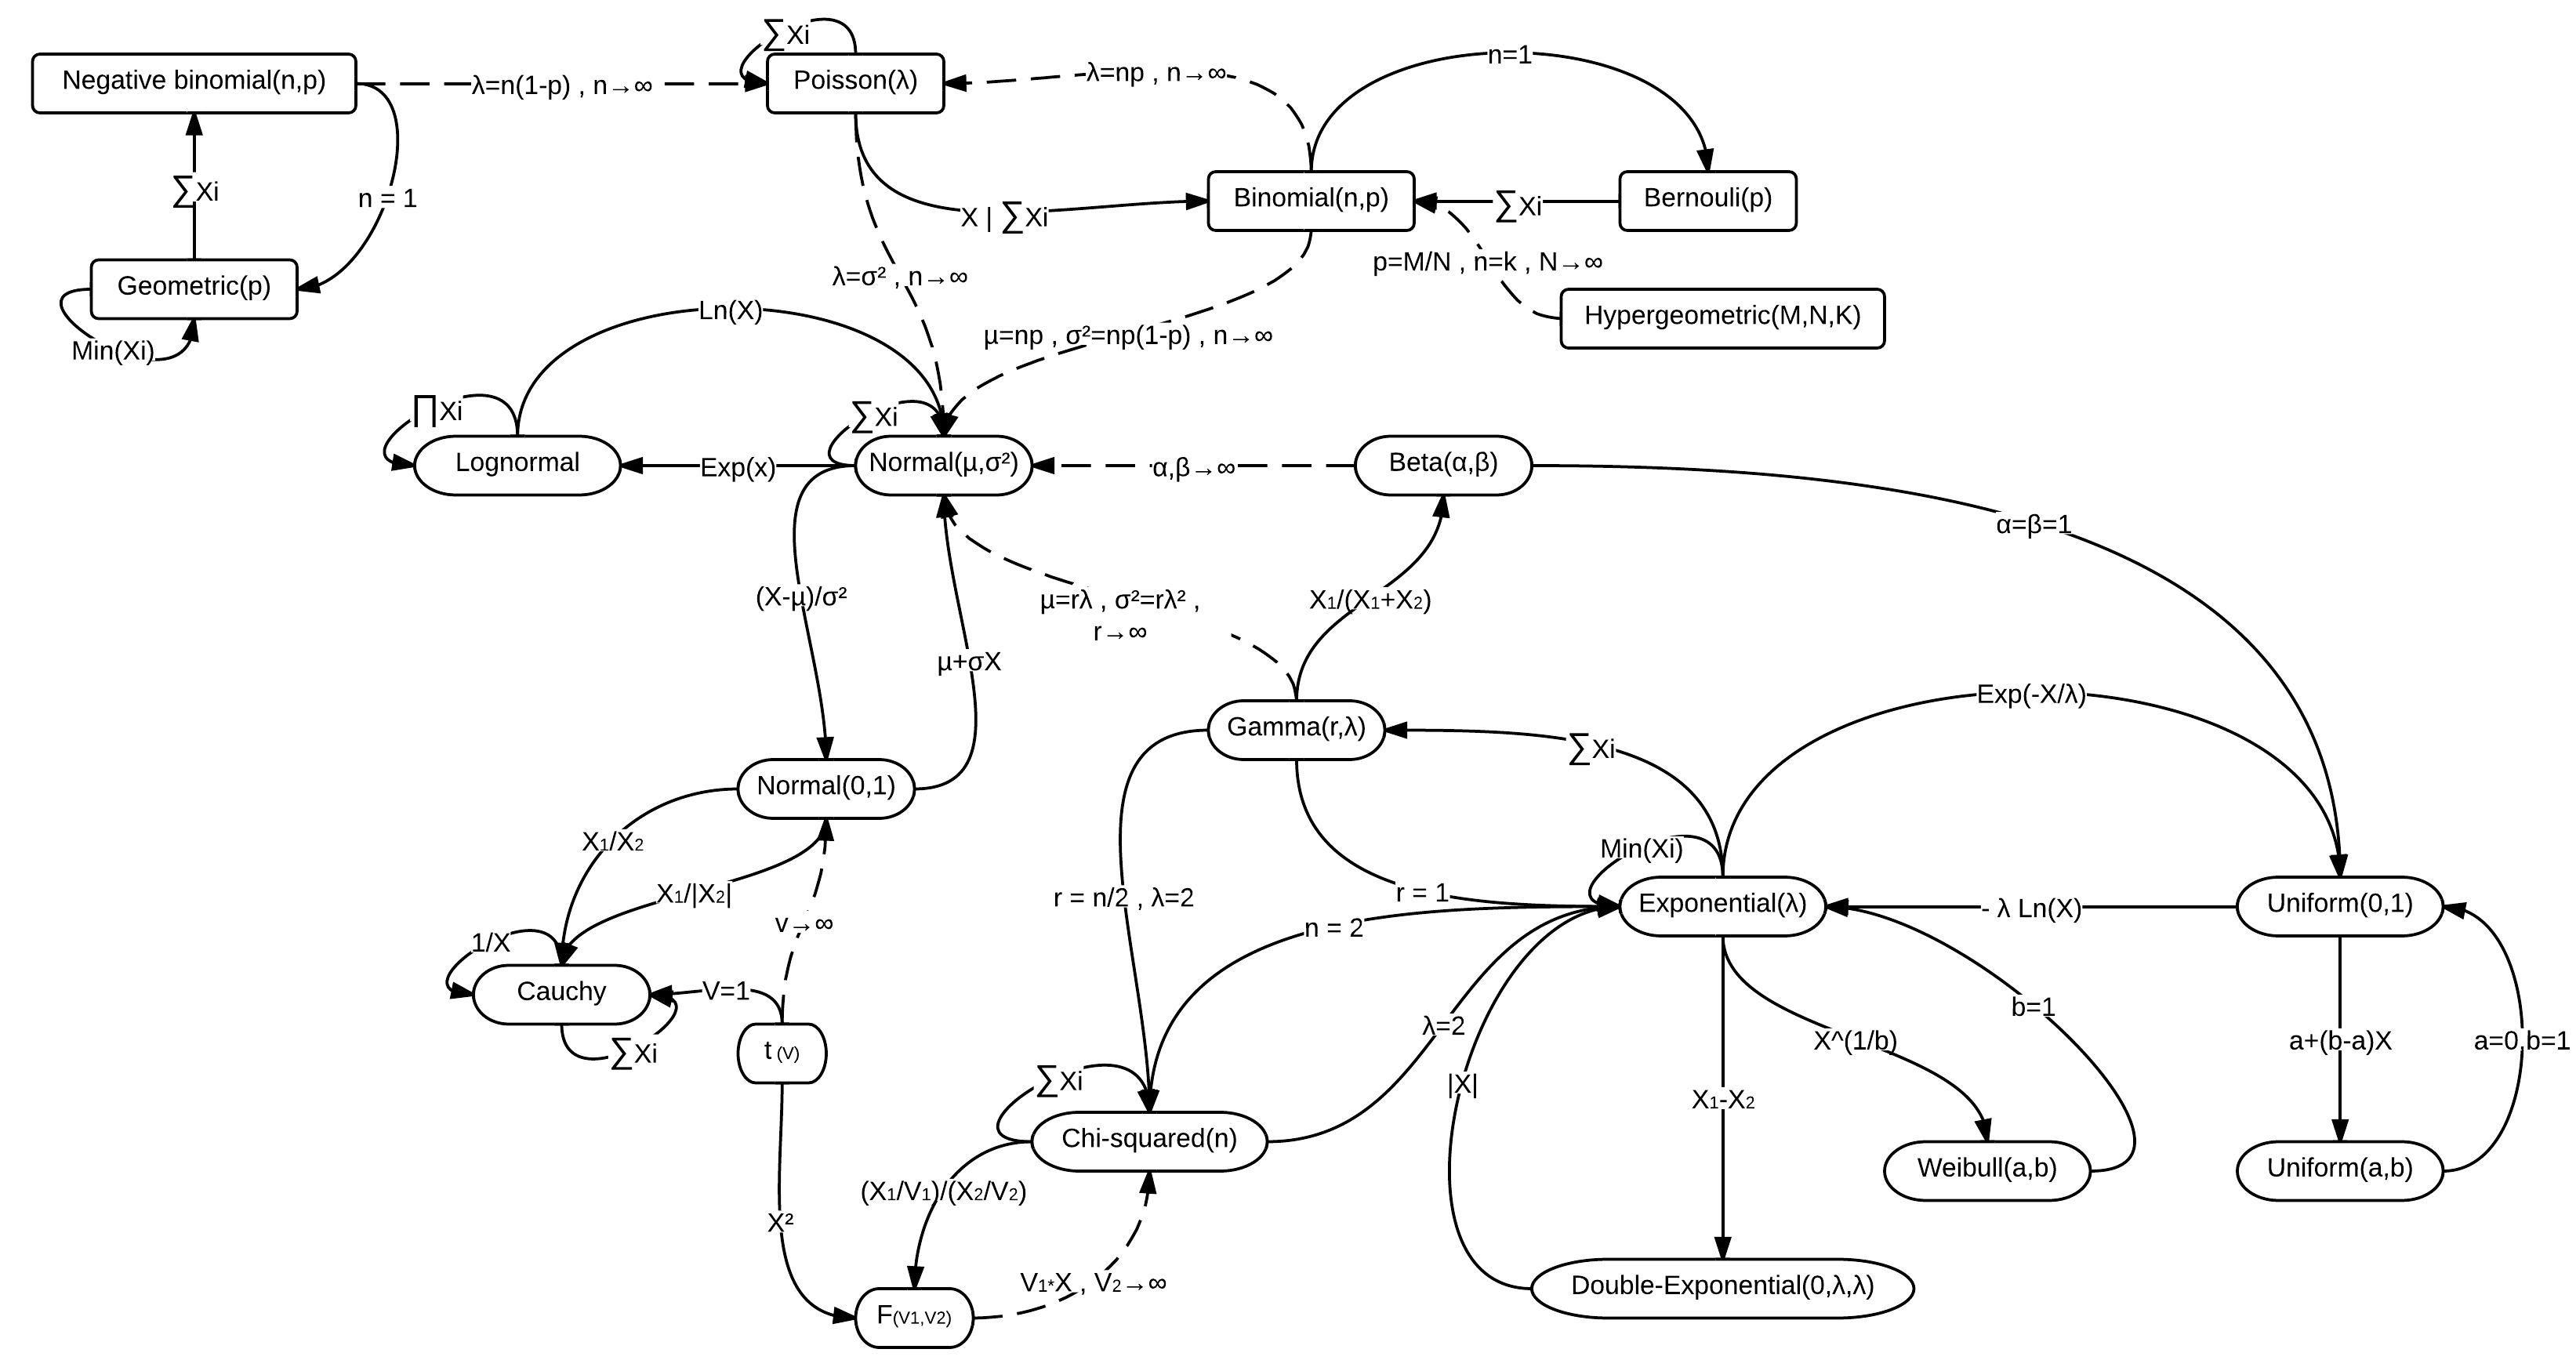
\includegraphics[scale=0.63]{Figures/RelacionesProbabilidad}
    \decoRule
    \caption[Relaciones entre algunas de las distribuciones de probabilidad univariadas]{Las relaciones entre algunas de las distribuciones de probabilidad univariadas se ilustran con líneas conectadas, las líneas discontinuas significan relación aproximada. [Fuente: \parencite{univariateDist}}
    \label{fig:relacionesDistribuciones}
\end{figure}

\subsection{Procesos de Poisson}

Los procesos de Poisson son altamente utilizados para representar o modelar fenómenos en las telecomunicaciones, p. ej. la generación de llamadas telefónicas.\newline

Algunas propiedades de los procesos de Poisson son las siguientes \parencite{ PoissonMedium}:

Se compone de una secuencia de variables aleatorias $X1, X2, X3, ... Xk$, de modo que cada variable representa el número de ocurrencias de algún evento, durante un intervalo de tiempo.\newline

Es un proceso estocástico. Cada vez que ejecuta el proceso de Poisson, producirá una secuencia de resultados aleatorios diferentes según alguna distribución de probabilidad.\newline

Es un proceso discreto. Los resultados del proceso de Poisson son el número de ocurrencias de algún evento en el período de tiempo especificado, que sin duda es un número entero, es decir, un número discreto.\newline

Tiene incrementos independientes. Lo que esto significa es que el número de eventos que el proceso predice que ocurrirá en cualquier intervalo dado, es independiente del número en cualquier otro intervalo disjunto. \newline

Las variables constitutivas del proceso de Poisson $X1, X2, X3, ... Xk$ tienen una distribución idéntica.\newline

Las variables constitutivas del proceso de Poisson $X1, X2, X3, ... Xk$ tienen una distribución de Poisson , que viene dada por la Función Masa de Probabilidad (PMF):

\begin{equation}
    P_{X}(k)=\frac{e^{-\lambda}*\lambda ^{k}}{k!}
    \label{eqn:Poisson}
\end{equation}

La fórmula anterior nos da la probabilidad de ocurrencia de $k$ eventos en unidad de tiempo, dado que la tasa de ocurrencia promedio es $\lambda$ eventos por unidad de tiempo.\newline

\subsubsection{Modelado de tiempos entre llegadas}

Los procesos de Poisson tienen una subestructura notable. Aunque el número de eventos ocurridos se modela usando una distribución de Poisson discreta, el intervalo de tiempo entre eventos consecutivos se puede modelar usando una distribución exponencial, que es una distribución continua \parencite{PoissonMedium}.\newline

Sean $X1, X2, X3, ... Xi$ variables aleatorias tales que:

$X1$ = el intervalo de tiempo entre el inicio del proceso y el primer evento, es decir, la primera llegada,\newline
$X2$ = el tiempo entre llegadas entre la primera y la segunda llegada,\newline
$X3$ = el tiempo entre llegadas entre la segunda y la tercera llegada , y así sucesivamente.\newline

La distribución de la variable aleatoria $Xk$ que representa el tiempo entre llegadas entre la llegada $(k-1) th$ y $(k) th$ es \parencite{PoissonMedium}:
\begin{equation}
    X_{k}=Exponential(\lambda)
    \label{eqn:expon}
\end{equation}
La Función Densidad de Probabilidad (PDF) de la variable aleatoria $X_{k}$ es la siguiente:
\begin{equation}
    P_{X}(t)=\lambda e^{-\lambda t}
    \label{eqn:pdfexpon}
\end{equation}
Y describe la PDF de tiempos entre llegadas en un proceso de Poisson.

%----------------------------------------------------------------------------------------
%	SECTION 
%----------------------------------------------------------------------------------------

\section{MODELADO DEL CANAL CELULAR}

Los modelos de propagación por radio se clasifican en modelos a gran escala y a pequeña escala. Los efectos a gran escala generalmente ocurren en el orden de cientos a miles de metros de distancia. Los efectos a pequeña escala se localizan y ocurren temporalmente (en el orden de unos pocos segundos) o espacialmente (en el orden de unos pocos metros). Los parámetros del canal generalmente se dividen en Pérdida por trayectoria (PL), parámetros de gran escala (LSP, como sombreado, dispersión de retardo, dispersión angular, etc.) y parámetros de pequeña escala (como demora, ángulo de llegada y salida, etc.), que reflejan conjuntamente las características de desvanecimiento del canal. El procedimiento de generación de los coeficientes del canal se puede apreciar en la \textit{Figura~\ref{fig:Procedimiento de generacion de coeficientes de canal} }. La pérdida de ruta generalmente se expresa en una o dos fórmulas y un conjunto de valores numéricos de parámetros, que reflejan las relaciones con el entorno de transmisión, la distancia y la frecuencia, etc. \newline

\begin{figure}[th]
\centering
\includegraphics[scale=0.8]{Figures/Procedimiento de generación de coeficientes de canal}
\decoRule
\caption[Procedimiento de generación de coeficientes de canal]{Procedimiento de generación de coeficientes de canal, [Fuente: 3GPP TR36.873]}
\label{fig:Procedimiento de generacion de coeficientes de canal}
\end{figure}

El rendimiento a nivel de enlace es un fenómeno de pequeña escala el cual lidia con cambios instantáneos en el canal a través de áreas e instantes de tiempo pequeños donde se considera la potencia recibida como constante, por otra parte, en las simulaciones a nivel de sistema para determinar el rendimiento en general del sistema para un gran número de usuarios esparcidos en una área geográfica es necesario incorporar parámetros de larga escala como el comportamiento estadístico de la interferencia, así como los niveles de señal experimentados por cada usuario a través de largas distancias, ignorando las características transitorias del canal (las de pequeña escala) \parencite{Tranter2003}. En una simulación a nivel de sistema, principalmente se busca la probabilidad de que un usuario en particular alcance un servicio aceptable en el sistema, para esto es necesario contemplar los efectos de los múltiples usuarios para cada enlace individual entre un móvil y la estación base. Por lo tanto en las simulaciones a nivel de sistema se suelen omitir los parámetros a pequeña escala.\newline

\subsection{Relaciones Generales de Propagación}

La pérdida por trayectoria $L_p\ $ se define como \parencite{Correia2018}:

\begin{equation}
L_{p[dB]}=P_{tx[dBm]}+G_{tx[dBi]}-P_{rx\left[dBm\right]}+G_{rx\left[dBi\right]}
\label{eqn:Lp}
\end{equation}

Donde:\newline
\[P_{tx}\to Potencia\ de\ la\ antena\ transmisora\ \] 
\[G_{tx}\to Ganancia\ de\ la\ antena\ transmisora\ \] 
\[P_{rx}\to Potencia\ de\ la\ antena\ receptora\ \ \] 
\[G_{rx}\to Ganancia\ de\ la\ antena\ receptora\ \ \] 

En muchas aplicaciones la ganancia de la antena es referida al dipolo de media longitud de onda:\newline

\begin{equation}
G_{[dBi]} = G_{[dBd]}+{2.15} 
\label{eqn:Gain}
\end{equation}

La Potencia Isotrópica Radiada Efectiva (EIRP) se define como:

\begin{equation}
P_{EIRP[dBm]}=P_{tx\left[dBm\right]}{\ +\ G}_{tx[dBi]}
\label{eqn:EIRP}
\end{equation}

\subsection{Pérdida por trayectoria en el Espacio Libre (FSPL, \textit{Free Space Path Loss})}

El receptor puede recibir una señal atenuada directa (también llamada señal de línea de vista (LoS)) del transmisor. El FSPL se utiliza para predecir la pérdida de trayectoria cuando hay un LoS claro y sin obstrucciones entre el transmisor y el receptor. Se basa en la ley de distancia al cuadrado inverso que establece que la potencia recibida (PRX) decae por un factor de cuadrado de la distancia (d) desde el transmisor.\newline

Se considera a la propagación en el espacio libre como la mínima atenuación que una señal puede sufrir en el medio.\newline

La potencia de la señal receptora ${\ P}_{rx}$ con una propagación en el espacio libre se define como (también conocida como Formula de Friis):\newline

\begin{equation}
P_{rx\left[W\right]}={\left(\frac{{\lambda }_{[m]}}{4\pi d_{[m]}}\right)}^2P_{tx\left[W\right]}G_{tx}G_{rx}  
\label{eqn:Friis}
\end{equation}

ó\newline

\begin{equation}
P_{rx\left[dBW\right]}=-32.44+P_{tx\left[dBW\right]}+G_{tx\left[dBi\right]}+G_{rx\left[dBi\right]}-20{\mathrm{log} \left(d_{\left[km\right]}\right)\ }-20{\mathrm{log} \left(f_{\left[MHz\right]}\right)\ }
\label{eqn:Friss_dB}
\end{equation}

Donde:\newline
\[d\to Distancia\ entre\ Rx\ y\ Tx\ \] 
\[f\to Frecuencia\ de\ operaci\textrm{ó}n\ \] 
\[\lambda \to Longitud\ de\ onda,\ \ \ \ \ \ \ \ \lambda =\frac{c}{f}\ \] 
\[c\to Velocidad\ de\ la\ luz\ (\mathrm{299\ 792\ 458\ m/s})\] 

Por lo tanto, la pérdida por trayectoria en el espacio libre $L_0$ se define como:\newline

\begin{equation}
L_{0[dB]}=32.44+20{\mathrm{log} \left(d_{\left[km\right]}\right)\ }+20\mathrm{log}\mathrm{}(f_{[MHz]})
\label{eqn:L0}
\end{equation}

Tomando el modelo del decaimiento de potencia promedio con la distancia $a_{pd}$:\newline
\begin{equation}
L_{p[dB]}=L_{ref}+10a_{pd}{\mathrm{log} \left(d_{\left[km\right]}\right)\ }
\label{eqn:Lp_ref}
\end{equation}

\[a_{pd}=2,\ \ \ para\ una\ propagacion\ en\ el\ espacio\ libre\ \] 

El \textit{apd (también conocido como PLE)} es un valor que va de 2 a 4 frecuentemente. El valor mínimo (i.e. 2) proviene de la perdida FSPL y el máximo (i.e. 4) por la pérdida del modelo \textit{Flat Earth} (modelo de tierra plana). En algunos modelos se llega a incluir valores de PLE más altos que los aquí definidos.\newline

\subsection{Caracterización del canal de radio}

Usualmente en ambientes urbanos no hay línea de vista (LoS) entre la estación base (BS) y la terminal móvil (MT\footnote{MT y UE son términos análogos.}) \textit{[véase Figura~\ref{fig:Propagacion}]} por lo que la transmisión es realizada por reflexión, difracción y dispersión de las señales.\newline

\begin{figure}[th]
\centering
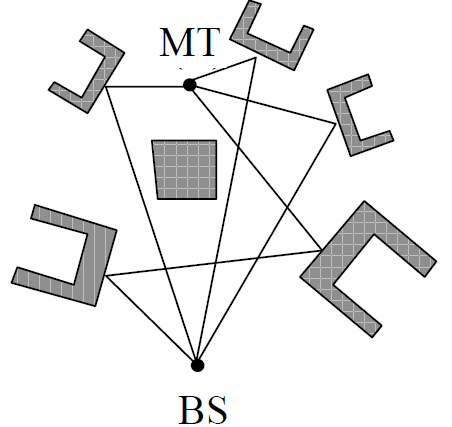
\includegraphics[scale=.5]{Figures/Propagación de señales celulares en ambientes urbanos.}
\decoRule
\caption[Propagación de señales celulares en ambientes urbanos]{Propagación de señales celulares en ambientes urbanos, [Fuente: L. Correia 2018]}
\label{fig:Propagacion}
\end{figure}

Sin embargo estas señales sufren de desvanecimiento con caídas de potencia. Este desvanecimiento depende de la posición y el ambiente del cual se propague la señal.\newline
Características de desvanecimiento:\newline

\begin{itemize}
    \item Desvanecimiento lento:
    Depende esencialmente de la distancia, sigue una distribución Log-normal
    \item Desvanecimiento rápido:
    Es asociado al movimiento del usuario, sigue una distribución Rice
\end{itemize}

\begin{figure}[th]
\centering
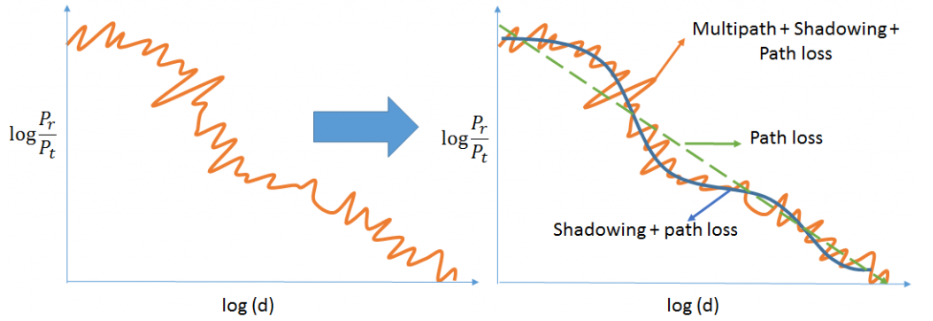
\includegraphics[scale=.8]{Figures/Ejemplo de niveles de señal con desvanecimiento lento y desvanecimiento rápido}
\decoRule
\caption[Ejemplo de niveles de señal con desvanecimiento lento y desvanecimiento rápido]{Ejemplo de niveles de señal con desvanecimiento lento y desvanecimiento rápido, [Fuente: V. Mathuranathan, 2016]}
\label{fig:Desvanecimientos}
\end{figure}

En la \textit{Figura~\ref{fig:Desvanecimientos}} se observa que al principio, la señal parece muy aleatoria. Mirando más de cerca podemos dividirlo en tres componentes principales como se muestra en la mitad derecha de la \textit{Figura~\ref{fig:Desvanecimientos}} \parencite{Mathuranathan2016}.\newline

\begin{enumerate}
    \item  Pérdida por trayectoria \textit{(Path loss)}
    \item  \textit{Shadowing} (Sombreado) o desvanecimiento lento
    \item  Desvanecimiento multitrayectoria o desvanecimiento rápido.
\end{enumerate}

El desvanecimiento lento puede ser causado por eventos como el \textit{shadowing}, donde una gran obstrucción, como una colina o un gran edificio, oscurece la trayectoria de la señal principal entre el transmisor y el receptor. Se considera un parámetro a gran escala.\newline

El desvanecimiento rápido ocurre cuando la amplitud y el cambio de fase impuestos por el canal varían considerablemente durante el período de uso. Una señal que viaja en un entorno puede verse reflejada por varios objetos en el camino. Esto da lugar a varias señales reflejadas. Las señales reflejadas llegan al receptor en diferentes instantes de tiempo y con diferentes intensidades que conducen a la propagación multitrayectoria. Se considera un parámetro a pequeña escala.\newline

Los márgenes de desvanecimiento deben tomarse en cuenta para caracterizar la variación de las señales alrededor de un valor promedio, esto depende de:\newline
•	Características del ambiente (LoS)\newline
•	QoS\newline

Para \textit{narrowband} (banda estrecha, donde prevalece el desvanecimiento plano en lugar de un desvanecimiento selectivo de frecuencia) el desvanecimiento se caracteriza de la siguiente manera:
\begin{itemize}
    \item Desvanecimiento rápido:
    \begin{itemize}
        \item LoS: Distribución Rice (no intenso)
        \item NLoS: Distribución Rayleigh (intenso)
    \end{itemize}
    \item Desvanecimiento lento:
    \begin{itemize}
        \item Distribución Log-Normal
    \end{itemize}
    \item Ambos desvanecimiento rápido y lento:
    \begin{itemize}
        \item Distribución Susuki
    \end{itemize}
\end{itemize}

Los modelos de estimación de señal pueden ser divididos en dos categorías:
\begin{enumerate}
    \item Teóricos:Son una aproximación a la realidad, no toman en cuenta todos los factores de la propagación pero permiten cambios fáciles de los parámetros. 
    \begin{itemize}
        \item Ray Tracing
        \item Modelo Ikegami [1984]
        \item Modelo Walfish-Bertoni [1988]
    \end{itemize}
    \item Empíricos: Están basados en la observación de mediciones, conduciendo al mejor ajuste de ecuaciones. Tienen la ventaja de tomar en cuenta todos los factores que influyen en la propagación.\newline
    Para ambientes exteriores hay dos modelos básicos:\newline
    \begin{itemize}
        \item COST 231 Okumura-Hata
        \begin{itemize}
            \item Largas distancias (>5km)
            \item Ambientes rurales, urbanos y suburbanos
            \item Alta desviacion estandar
            \item Rango de frecuencias aplicables [1.5,2.0] GHz
        \end{itemize}
        \item COST 231 Walfish-Ikegami [1999]
        \begin{itemize}
            \item Cortas distancias (<5km)
            \item Ambientes urbanos y suburbanos
            \item Rango de frecuencias aplicables [.8,2.0] GHz
        \end{itemize}
        \item COST 207 [1989]
    \end{itemize}
\end{enumerate}

%----------------------------------------------------------------------------------------
%	SECTION 
%----------------------------------------------------------------------------------------

\section{GEOMETRÍA CLÁSICA CELULAR}

Los sistemas celulares brindan una determinada cobertura para un servicio, dividiendo el área geográfica en segmentos llamados celdas donde el espectro de frecuencia también es dividido en canales y estos son agrupados para repartirse entre las celdas. Estos sistemas logran una alta capacidad gracias al reúso del canal de comunicación permitiendo a las estaciones base compartir los canales, sin embargo, este reúso da como resultado una interferencia co-canal generada solamente entre usuarios que comparten el mismo canal, lo cual limita el rendimiento y capacidad de un sistema celular dado que los efectos de esta interferencia son altamente dependientes con los aspectos del sistema \parencite{Tranter2003} como lo son el tipo de acceso múltiple del sistema, el número de usuarios compartiendo el canal, el canal de propagación, la perdida por trayectoria, el desvanecimiento, entre otros.\newline

\begin{itemize}
    \item Ser limitados por la interferencia (capacidad).
    \item Servir a una alta densidad de usuarios.
    \item Considerar la disponibilidad del espectro solo como un factor limitante.
    \item Reúso de frecuencias.
    \item Uso de Estaciones Base de baja potencia.
    \item Tener celdas de distintas coberturas.
    \item Permitir \textit{handover}.
\end{itemize}

\subsection{Planeación Celular}

Una buena planeación celular es de crucial importancia para lograr un buen rendimiento del sistema y la provisión de una buena Calidad de servicio (QoS).\newline

La planeación celular consiste en:\newline
\begin{itemize}
    \item Colocación de BSs y establecimiento de coberturas
    \item Optima administración de recursos de radio.
    \item Minimización de interferencia.
\end{itemize}

La planeación celular se desempeña de acuerdo a:\newline
\begin{itemize}
    \item Morfología del área de servicio y modelos de propagación.
    \item Perfiles de usuario y modelos de tráfico.
\end{itemize}
Considerando:\newline

\[R\to Radio\ de\ cobertura\ de\ la\ celda\] 
\[D_r\to Distancia\ de\ reuso\ de\ celda\ co\_canal\] 
\[d_u\to Distancia\ unitaria\ entre\ los\ centros\ de\ dos\ celdas\ adjacentes\] 
\[d_u=\sqrt{3}R\] 
\[Llegando\ a\ una\ distancia\ de\ reuso\ normalizada\ D_n\] 

\begin{equation}
D_n=i^2+ij+j^2, donde: i!=0, j!=0
\label{eqn:DistReuso}
\end{equation}

\begin{equation}
=>\ D_r=D_nd_u
\label{eqn:Dn}
\end{equation}

\[\textrm{á}rea\ de\ una\ celda\ S_{cel}\] 

\begin{equation}
S_{cel}=(3\sqrt{3}/2)R^2
\label{eqn:S}
\end{equation}

\[\textrm{á}rea\ de\ un\ cluster\ S_{clu}\] 

\begin{equation}
S_{clu}=(3\sqrt{3}/2)D^2_nd^2_u
\label{eqn:Sclus}
\end{equation}

\[Número\ de\ celdas\ por\ cluster,\ N_{cc}\ \textrm{ó}\ tambi\textrm{é}n\ conocido\ como\ ``factor\ de\ reuso''\ \] 

\begin{equation}
N_{cc}=\frac{S_{clu}}{S_{cel}}
\label{eqn:N}
\end{equation}

$Siendo\ valores\ posibles\ para\ N_{cc}\ ,\ \ \ \ 1,\ 3,\ 4,\ 7,\ 9,\ 12,\ 13,\ .\ .\ .\ $\textit{[Véase Figura~\ref{fig:clusterizacion} y Figura~\ref{fig:celdascocanal}]}\newline

Para implementar el reúso, se deben asignar un conjunto de canales disponibles para un grupo de celdas, el clúster y repetir ese conjunto a través de toda el área de servicio.\newline

\begin{equation}
N_{ch/c}=\frac{N_{ch/s}}{N_{cc}} 
\label{eqn:Nch}
\end{equation}

\[N_{ch/c}\to Numero\ de\ canales\ por\ celda\] 
\[N_{ch/s}\to \ Numero\ de\ canales\ en\ el\ sistema\] 
\[N_{cc}\to Numero\ de\ celdas\ por\ cluster\ \] 

La relación de reutilización co-canal,$\ r_{cc}\ $es usada para caracterizar clústeres\newline
\begin{equation}
r_{cc}=\frac{D_r}{R}=\sqrt{3N_{cc}}
\label{eqn:}
\end{equation}

Un valor grande de $r_{cc}$ corresponde a:\newline
\begin{enumerate}
\item  Una baja interferencia co-canal
\item  Baja capacidad del sistema
\end{enumerate}

El clúster es escogido lo más pequeño posible tomando los umbrales de interferencia en consideración \parencite{Correia2018}.\newline
\[GSM,\ {N}_{cc}=4\] 
\[UMTS,\ {N}_{cc}=1\] 
\[LTE,\ {N}_{cc}=3\] 

\begin{figure}[th]
\centering
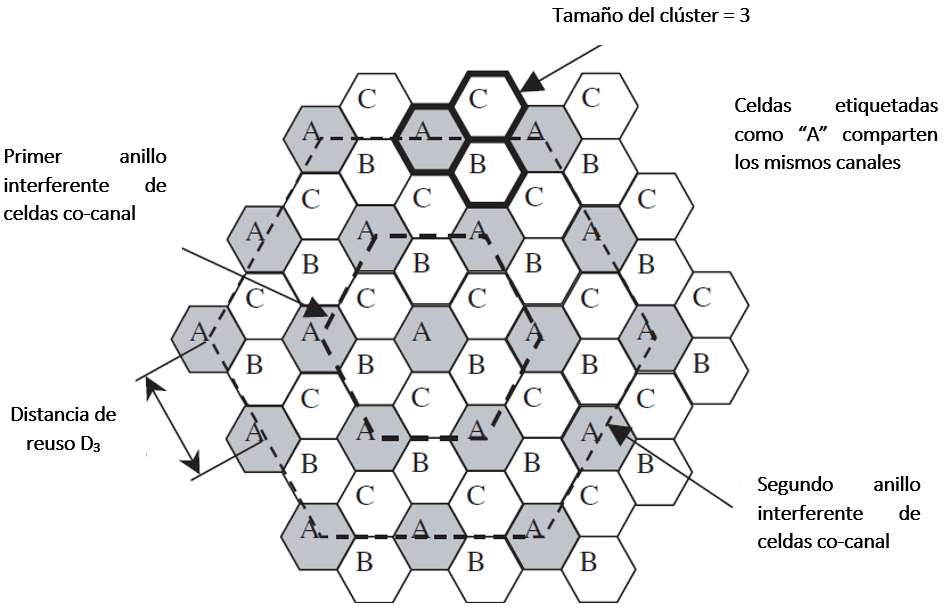
\includegraphics[scale=.4]{Figures/Clusterización de celdas con un factor de reúso de 3 celdas}
\decoRule
\caption[Clusterización de celdas con un factor de reúso de 3 celdas]{Clusterización de celdas con un factor de reúso de 3 celdas, [Fuente: Tranter 2003]}
\label{fig:clusterizacion}
\end{figure}

\begin{figure}[th]
\centering
\includegraphics[scale=.5]{Figures/Localización de celdas co-canal con distintos factores de reuso}
\decoRule
\caption[Localización de celdas co-canal con distintos factores de reúso]{Localización de celdas co-canal con distintos factores de reúso, [Fuente: Tranter 2003]}
\label{fig:celdascocanal}
\end{figure}

Diferentes tamaños de celda son usadas para distribuciones no uniformes de tráfico \parencite{TurjmanSmallCells}.\newline

\begin{figure}[th]
\centering
\includegraphics[scale=.3]{Figures/Sistema celular con celdas de tamaño no uniforme}
\decoRule
\caption[Sistema celular con celdas de tamaño no uniforme]{Sistema celular con celdas de tamaño no uniforme, [Fuente: Yacoub 1993]}
\label{fig:nouniformcells}
\end{figure}

El uso de diferentes tamaños de celdas:\newline
•	Conduce a un incremento de interferencia, debido a la poca uniformidad en la estructura celular.\newline
•	Requiere cuidado adicional en el despliegue de BSs\newline

\subsection{Planeación de frecuencia}
La decisión de bandas de frecuencia para ser usadas en los diversos sistemas de comunicaciones es decidida por la ITU. La asignación de canales en una banda dada para un operador es decidido a nivel nacional por un cuerpo regulatorio, IFT en México. El hecho de que el espectro es muy escaso incita a un eficiente uso de frecuencias.\newline

El número de frecuencias (portadoras, canales de radio) por celda $N_{fc}$ depende del clúster, $N_{cc}$, y del número de frecuencias en el sistema $N_{fs}$
\begin{equation}
    N_{fc}={N_{fs}}/{N_{cc}}
    \label{eqn:Nfc}
\end{equation}

Debido a la limitación en el número de frecuencias, debe haber una compensación entre la interferencia $N_{cc}\ $y la capacidad$\ N_{ch/c}\ $en el sistema.\newline

La asignación de frecuencias de las celdas debería reducir la interferencia de celda-adyacente maximizando la separación de las frecuencias en una celda.\newline

En un simple sistema celular, las frecuencias deberían ser asignadas a las celdas de acuerdo a:\newline
\begin{equation}
    f_{ij}=i+N_{cc}\ (j-1)
    \label{eqn:fij}
\end{equation}

\[i=1,\ \dots ,\ N_{cc}\] 
\[j=1,\ \dots ,\ N_{fc}\] 

Cuando $N_{sc}$ sectores por celdas son implementados, cada sector deberá contener su propio grupo de frecuencias:\newline
\begin{equation}
    f_{ijk}=i+N_{cc}\ \left(k-1\right)+N_{cc}\ N_{sc}\ (j-1)
    \label{eqn:fijk}
\end{equation}

\[i=1,\ \dots ,\ N_{cc}\] 
\[j=1,\ \dots ,\ N_{fc}\] 
\[k=1,\ \dots ,\ N_{sc}\] \\

%----------------------------------------------------------------------------------------
%	SECTION 
%----------------------------------------------------------------------------------------

\section{INTERFERENCIA EN SISTEMAS CELULARES}

En general el receptor recibe:\newline
\begin{equation}
\mathrm{SNIR=}\frac{S}{I+N}
\label{eqn:SNIR}
\end{equation}

Donde:
\[S\to Potencia\ de\ portadora\ de\ la\ se\textrm{\~{n}}al\ deseada\] 
\[I\to Potencia\ de\ las\ portadoras\ de\ las\ se\textrm{\~{n}}alees\ interferentes\] 
\[N\to Potencia\ del\ ruido\] 

Los sistemas de comunicaciones móviles se caracterizan por ser sistemas limitados por interferencia, donde I domina sobre N, por lo tanto la participación del ruido N puede ser ignorada \parencite{Correia2018}.\newline
Quedando entonces como la relación portadora a interferencia:\newline
\begin{equation}
\frac{S}{I+N}\ \ \cong \ \ \frac{S}{I}\ \ \to \ \ SIR
\label{eqn:SIR}
\end{equation}

La interferencia co-canal $I_{cc}$ es un problema aceptado en los sistemas de comunicaciones móviles. \newline

La estimación de la relación portadora a interferencia co-canal ${S}/{I_{cc}}$es calculada de acuerdo  a las siguientes asunciones:

\begin{enumerate}
\item  Todas las celdas son del mismo tamaño
\item  La potencia radiada por todas las BSs son iguales
\item  Todas las BSs tienen antenas omnidireccionales
\item  El decaimiento de la potencia promedio ($a_{pd}$) con la distancia es de la forma:
\end{enumerate}

\begin{equation}
P_r=P_0{(d/d_0)}^{-a_{pd}} 
\label{eqn:P_r}
\end{equation}

En un sistema celular en general, la interferencia co-canal es calculada tomando la interferencia de todas las celdas $N_{Icc}$\newline
\begin{equation}
\frac{S}{I_{cc}}\ =\ \ \frac{S}{\sum^{N_{Icc}}_{k=1}{I_k}} 
\label{eqn:Icc}
\end{equation}

Usualmente la interferencia puede ser estimada por tomar únicamente el primer anillo de interferencia \parencite{Correia2018}.\newline
\begin{equation}
\frac{S}{I_{cc}}\ =\ \ \frac{S}{\sum^6_{k=1}{I_k}} 
\label{eqn:I}
\end{equation}

Para el caso de transmisión de bajada \textit{downlink} para un usuario en los límites de la celda, el cálculo de la interferencia co-canal se puede aproximar a:\newline
\begin{equation}
    \frac{S}{I_{cc}}=\frac{R^{-a_{pd}}}{ 2(D_{r}-R)^{-a_{pd}}+2(D_{r})^{-a_{pd}} + 2(D_{r}+R)^{-a_{pd}}}\\
    \label{eqn:SIcc}
\end{equation}

Donde:\\
$R$ : radio de cobertura de la celda\\
$D_{r}:$ distancia de reuso de celda co-canal\\

La interferencia puede disminuir \parencite{Correia2018}:
\begin{itemize}
    \item implementando celdas sectorizadas.
    \item \textit{downtilting} el lóbulo principal de la antena de la BS.
    \item bajando la altura de la BS
    \item optimizando la localización de la BS
    \item implementando control de potencia
    \item implementando \textit{frequency hopping }
\end{itemize}

En resumen, la planeación de una red celular de radio es ejecutada de la siguiente manera:\newline
\begin{enumerate}
    \item El mínimo valor para la relación portadora a interferencia impone el tamaño del clúster.
    \item Se estima el tráfico en una celda determinada.
    \item Se calcula el número de canales para una calidad de servicio determinada.
    \item En caso de que el número de canales disponibles no sea suficiente, el tráfico se reducirá, es decir, la cobertura se reducirá.
    \item Se establece el plan de frecuencias y la estructura del despliegue de celdas.
    \item Cuando se propone una estructura de celdas no uniforme, los canales deberán ser distribuidos de acuerdo a las necesidades de capacidad, y a los valores topes permitidos de interferencias co- canal y canal-adyacente.
\end{enumerate}\


%----------------------------------------------------------------------------------------
%	SECTION 
%----------------------------------------------------------------------------------------

\section{CAPACIDAD EN SISTEMAS DE COMUNICACIONES}

La teoría de la información de Shannon nos dice la cantidad de información que un canal puede transportar. En otras palabras, especifica la capacidad del canal. La capacidad de un sistema de comunicación es la velocidad de datos máxima en bits por segundo que se puede transferir de manera confiable del transmisor al receptor. En el sentido estricto de la teoría de la información, este es un límite superior insuperable que, en la práctica, solo se puede abordar. En un único enlace Tx-Rx de ancho de banda de unidad sujeto a AWGN, la capacidad en bits por uso de canal (es decir, bps / Hz) viene dada por la fórmula de \emph{Shannon-Hartley}:\newline

\begin{equation}
C=B{{\mathrm{log}}_2 \left(1+\frac{S}{N}\right)\   [bps] }
\label{eqn:Shannon}
\end{equation}
\[B\ es\ el\ ancho\ de\ banda\ del\ canal\ en\ Hertzios.\]
\[C\ es\ la\ capacidad\ del\ canal\ (tasa\ de\ bits\ de\ informaci\textrm{ó}n\ bit/s)\]
\[S\ es\ la\ potencia\ de\ la\ se\textrm{\~{n}}al\ \textrm{ú}til\ (W,\ mW,\ etc.)\]
\[N\ es\ la\ potencia\ del\ ruido\ presente\ en\ el\ canal,\left(W,\ mW,\ etc.\right),\ \ que\ trata\ de\ enmascarar\ a\ la\ se\textrm{\~{n}}al\ \textrm{ú}til.\] 


%----------------------------------------------------------------------------------------
%	SECTION 
%----------------------------------------------------------------------------------------

\section{INTERFAZ DE RADIO}

Los canales de transmisión dirigidos desde la BS a MT son referidos como canal \textit{downlink} y los dirigidos desde el MT a la BS como canales \textit{uplink}, estos canales juntos se identifican como canales ``dúplex'. La transmisión bidireccional de la información en sistemas dúplex puede dividirse en \parencite{Correia2018}:

\begin{enumerate}
\item  Frecuencia: Donde los canales UL y DL ocupan diferentes bandas de frecuencia - FDD (\textit{Frequency Division Multiplexing}).
\item  Tiempo: Donde los canales UL y DL ocupan diferentes ventanas de tiempo- TDD (\textit{Time Division Multiplexing}).
\end{enumerate}

FDD se caracteriza por: 
\begin{itemize}
\item  Cuando es utilizada una división ``dúplex'' de frecuencia FDD estos canales son transmitidos en diferentes frecuencias
\item  Permitir transmisión simultánea en ambos caminos
\item  Requieren filtros con un buen rechazo en la banda adyacente
\item  Requieren en general el uso de filtros dúplex
\end{itemize}

TDD se caracteriza por: 
\begin{itemize}
\item  Cuando se usa una división ``dúplex'' de tiempo TDD los canales son transmitidos en la misma frecuencia pero utilizando diferentes ranuras de tiempo.
\item  Permitir transmisión secuencial en ambos caminos
\item  Requiere sincronización
\item  No requieren uso de filtros dúplex
\end{itemize}

El uso de una técnica de división dúplex puede depender de la técnica de acceso múltiple utilizada para el sistema.

\subsection{Esquemas de Acceso Múltiple al Medio}
Las técnicas de acceso múltiple (MA) generalmente se pueden dividir en enfoques ortogonales y no ortogonales \parencite{Tse2004}. En MA ortogonal (OMA), los recursos de radio se dividen ortogonalmente entre dispositivos, donde las señales de diferentes dispositivos no se superponen entre sí. Las instancias de OMA son acceso múltiple por división de tiempo (TDMA), acceso múltiple por división de frecuencia (FDMA), acceso múltiple por división de frecuencia ortogonal (OFDMA), y FDMA de portadora única (SC-FDMA).\newline

Los enfoques OMA no tienen la capacidad de combatir la interferencia entre células \parencite{Shirvanimoghaddam2017}; por lo tanto, se requieren técnicas cuidadosas de planificación celular y gestión de interferencia para resolver este problema. \newline

Existen 4 técnicas básicas de acceso múltiple:

\begin{enumerate}
\item  frecuencia: asignación de una portadora - FDMA (Acceso múltiple por división de frecuencia)
\item  tiempo: asignación de un intervalo de tiempo - TDMA (Acceso múltiple por división de tiempo)
\item  código: asignación de un código - CDMA (Acceso múltiple por división de código)
\item   frecuencia ortogonal: asignación de un conjunto de sub-portadoras - OFDMA (Acceso múltiple por división de frecuencia ortogonal).
\end{enumerate}

 En muchos sistemas prácticos, se utiliza una mezcla o combinación de estas técnicas básicas \parencite{Correia2018}.\newline

\subsection{Generaciones anteriores de sistemas de comunicaciones móviles}

La generación 1G fue la primera generación de tecnología celular inalámbrica. 1G se introdujo en la década de 1980. Las señales de radio utilizadas por la red 1G fueron analógicas y proporcionaba comunicación solo por voz, alcanzaba una velocidad de 2.4 Kbps. La técnica de acceso múltiple utilizada en 1G es el acceso múltiple por división de frecuencia (FDMA) \parencite{Nair2018}. Esta generación utiliza el método de conmutación de circuitos para la transmisión de datos. \newline

Las redes celulares 2G de segunda generación fueron lanzadas comercialmente en el estándar GSM en Finlandia 1991 \parencite{Nair2018}. 2G utilizó el método de conmutación de paquetes para la transmisión de datos y habilitó el cifrado digital de la conversación por teléfono, además proporcionaron servicios multimedia como SMS (Servicios de mensajes cortos) MMS (Servicios de mensajes multimedia) y las velocidades de descarga y carga fueron de hasta 236 Kbps. Se utilizó el acceso múltiple por división de tiempo (TDMA), como el número de usuarios aumentó con el tiempo, TDMA se volvió obsoleto por causar una velocidad más baja para cada usuario.\newline

3G (conocida también como UMTS) fue la tercera generación de tecnología inalámbrica de telecomunicaciones móviles y utilizó el acceso múltiple por división de código de secuencia directa (DS-CDMA) \parencite{Nair2018}. Las redes 3G ofrecieron velocidades de 3.1 megabits por segundo (Mbps) o más y se instalaron por primera vez en 1998. La aplicación del concepto 3G se encuentra en telefonía inalámbrica, acceso a Internet móvil, acceso a Internet inalámbrico, llamadas de conferencia y TV portátil.\newline

\begin{figure}[th]
\centering
\includegraphics[scale=.6]{Figures/Diferentes tipos de acceso múltiple}
\decoRule
\caption[Diferentes tipos de acceso múltiple al medio ocupados en generaciones anteriores (1G, 2G y 3G)]{Diferentes tipos de acceso múltiple al medio ocupados en generaciones anteriores (1G, 2G y 3G), [Fuente: https://www.itu.int/osg/spuold/ni/3g/technology/index.html]}
\label{fig:MAs}
\end{figure}

4G (conocida también como LTE) es el término utilizado para describir la cuarta generación de servicio celular inalámbrico y es el estándar actual del servicio celular. Es hasta 10 veces más rápido que los servicios 3G. Sprint fue el primer operador en ofrecer velocidades 4G en los EE. UU a partir de 2009. Las redes 4G pueden ofrecer velocidades de descarga entre 5 y 12 Mbps y velocidades de carga entre 2 y 5 Mbps, lo que finalmente da una velocidad máxima de 50Mbps. El sistema de comunicación celular 4G utiliza una versión avanzada del esquema FDMA, es decir, OFDMA (acceso múltiple por división de frecuencia ortogonal) \parencite{Nair2018}.\newline

%----------------------------------------------------------------------------------------
%	SECTION 
%----------------------------------------------------------------------------------------

\section{REDES DE QUINTA GENERACIÓN (5G)}

La NGMN define su visión de una red 5G de la siguiente manera: "5G es un ecosistema de extremo a extremo para permitir una sociedad totalmente móvil y conectada."\newline

La anteriores generaciones de comunicaciones móviles (1G,{\dots},4G) han sido transformadoras en el sentido que fueron motivadas para mejorar los tradicionales KPIs de la red, sin embargo la nueva generación de comunicaciones móviles (5G) aparte de ser transformadora viene a ser disruptiva ante las generaciones anteriores ya que propone nuevas técnicas, modelos y KPIs que habilitarán una gama amplia de servicios con alta fiabilidad, ayudando a conformar toda una red heterogénea global móvil interconectada con altos índices de rendimiento.\newline

La investigación sobre los casos de uso de una red 5G y sus requisitos técnicos han sido realizadas por la ITU-R, el 3GPP y la NGMN:

\begin{figure}[th]
\centering
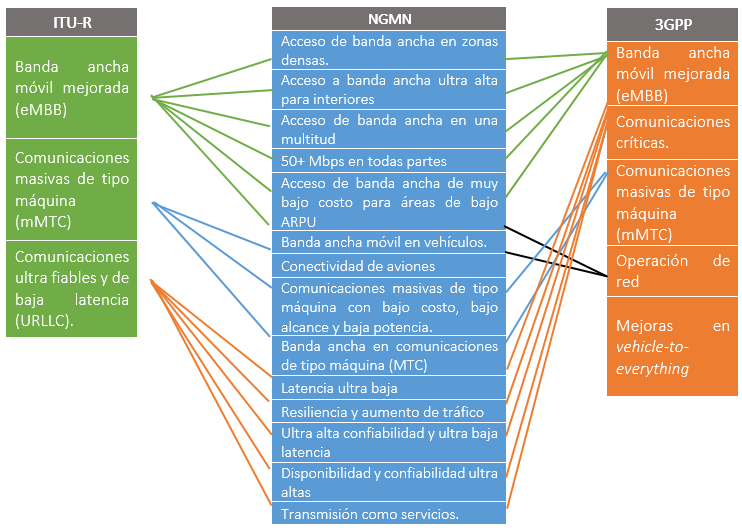
\includegraphics[scale=1]{Figures/Comparación de diversos escenarios de uso de la tecnología 5G}
\decoRule
\caption[Comparación de diversos escenarios de uso de la tecnología 5G por la UIT-R, el 3GPP y la NGMN]{Comparación de diversos escenarios de uso de la tecnología 5G por la UIT-R, el 3GPP y la NGMN}
\label{fig:5g}
\end{figure}

5G admitirá una gran variedad de casos de uso que están surgiendo ahora o surgirán en el futuro. Los diversos casos de uso tienen características y requisitos variables. Es útil agrupar innumerables casos de uso emergentes en varias familias de casos de uso. \newline

La \textit{Figura~\ref{fig:5g}} muestra las ocho familias de casos de uso por la NGMN con un ejemplo de caso de uso para cada familia, y sus correspondientes ejemplos de casos de uso con la 3GPP y la ITU-R.\newline

En términos generales, ITU-R ha concluido tres casos de uso para abordar la gran variedad de requisitos y características \parencite{5gMobileComms}:


\begin{enumerate}
    \item \textbf{Banda ancha móvil mejorada} \textbf{(eMBB)}: la banda ancha móvil aborda casos de uso centrados en el hombre para acceder a contenido multimedia, servicios y datos. La demanda de banda ancha móvil seguirá aumentando, lo que dará lugar a una banda ancha móvil mejorada. El escenario mejorado de uso de banda ancha móvil vendrá con nuevas áreas de aplicación y requisitos, además de las aplicaciones de banda ancha móvil existentes para un mejor rendimiento y una experiencia de usuario cada vez más perfecta.
    \item \textbf{Comunicaciones ultra fiables y de baja latencia (URLLC)}: este caso de uso tiene requisitos estrictos para capacidades tales como rendimiento, latencia y disponibilidad. Algunos ejemplos incluyen el control inalámbrico de la fabricación industrial o los procesos de producción, cirugía médica remota, automatización de la distribución en una red inteligente, seguridad en el transporte, manejo autónomo de automóviles, etc.
    \item \textbf{Comunicaciones masivas de tipo máquina (mMTC)}: este caso de uso se caracteriza por un gran número de dispositivos conectados que transmiten un volumen relativamente bajo de datos no sensibles al retardo. Los dispositivos deben ser de bajo costo y tener una batería de larga duración.
\end{enumerate}



%----------------------------------------------------------------------------------------
%	SECTION 
%----------------------------------------------------------------------------------------

\section{INTERNET DE LAS COSAS (IoT)}


El internet de las cosas (IoT) es una emergente y prometedora tecnología que habilitará la interconexión del mundo global a través de la conexión de objetos físicos (comúnmente dispositivos de bajo consumo) mediante el uso del internet \parencite{5GSurveyAkpaku}. Una de las características más importantes de esta tecnología es que ocupa la comunicación máquina a máquina (M2M) con el fin de que los dispositivos se conecten y comuniquen entre sí sin alguna intervención humana.\newline

Para habilitar esta tecnología se requiere el soporte para conexiones masivas, es decir, admitir la gran cantidad de sensores en una sola celda. Debido a que la mayoría de estos sensores deben operar durante varios años, la eficiencia energética en las transmisiones inalámbricas es un requisito importante. Además, se debe reducir el costo de implementación de tales sensores \parencite{IoT5GWire}.


%----------------------------------------------------------------------------------------
%	SECTION 
%----------------------------------------------------------------------------------------

\section{TELETRÁFICO}

Conceptos básicos:
\begin{enumerate}
\item  \underbar{Tráfico}: Es el acumulado de peticiones de servicio de todos los usuarios atendidos por la red o por una parte de ella.
\item  \underbar{Recurso o servidor}: medio físico, usualmente sólo es capaz de atender un solo servicio.
\item  \underbar{Sistema de colas}: conjunto de servidores de uso compartido.
\end{enumerate}

\subsection{Caracterización del Tráfico}
Para caracterizar el tráfico se deben definir previamente los siguientes conceptos:
\begin{enumerate}
\item  \underbar{Volumen de Tráfico Cursado}. Suma de la duración de todos los servicios atendidos por el sistema.
\item  \underbar{Intensidad de Tráfico Cursado u Ocupación promedio de recursos (a')}. Número promedio de servicios atendidos simultáneamente. Se puede obtener mediante dividir el volumen de tráfico cursado entre el tiempo que tomó cursar dicho volumen. También se puede interpretar como el número promedio de servidores ocupados.
\item  \underbar{Intensidad de Tráfico Ofrecido (a).} Número promedio de servicios atendidos simultáneamente, si todas las peticiones fueran atendidas.
\end{enumerate}

Suponiendo un sistema que es capaz de atender todas las peticiones de servicio y al que arriban $\lambda$ peticiones/segundo. Esto implica que en un intervalo T segundos se recibirían $\lambda$$\cdot$T peticiones de servicio. Si la duración promedio de estos servicios es $\mu$ segundos, entonces el volumen de tráfico ofrecido (y en este caso también cursado) es $\lambda$$\cdot$$\mu$$\cdot$T y la intensidad de tráfico ofrecido se reduce a:
\begin{center}
$a=\lambda\cdot\mu$
\end{center}

Para un sistema que atiende todas las peticiones el tráfico cursado y el ofrecido son iguales, sin embargo, cuando se analizan sistemas que no cumplan esta característica, a se vuelve un valor hipotético (la intensidad de tráfico cursado, si todas las peticiones se atendieran), sin embargo, seguirá describiendo la intensidad del tráfico que se ofrece. Es importante mencionar que el desempeño de un sistema (en términos de algún parámetro de calidad de servicio) no va a depender del valor de $\lambda$ o de $\mu$ por sí solos, sino del producto de ellos. Por ejemplo, un sistema se puede saturar tanto por una alta tasa de arribos como por una gran duración del tiempo de servicio.\newline

Hasta este punto el tráfico sólo se ha caracterizado en término de dos valores promedio: la tasa de arribos ($\lambda$) y la duración promedio de los servicios ($\mu$). Estos parámetros representan información parcial de dos variables aleatorias, el tiempo entre arribos (TEA) y el tiempo duración de servicio (TDS). Estos tiempos por su carácter aleatorio en muchos análisis se modelan como variables aleatorias. El tipo de comportamiento aleatorio en las tasas se establece al de una distribución exponencial negativa \parencite{Carter1990}. La tasa de arribos corresponde una distribución como sigue:
\begin{equation}
f(y)=\lambda e^{-\lambda y}\cdot u(y)
\label{eqn:lambda}
\end{equation}

La duración promedio de servicios corresponde a:
\begin{equation}
f(y)=\frac{1}{\mu } e^{-\frac{1}{\mu} y} \cdot u(y)
\label{eqn:mu}
\end{equation} 

Es necesario establecer fórmulas que relacionen a la cantidad de recursos y el tráfico ofrecido con los parámetros de calidad de servicio, se requiere como paso intermedio determinar la probabilidad de que el sistema se encuentre en determinado estado.\newline

Se considera que el sistema está en estado j, si la suma de los servicios que están siendo atendidos más los servicios en espera es j.\newline

Una técnica que simplifica significativamente el cálculo de las probabilidades de estado es el uso de cadenas de Markov, sin embargo, la solución mediante este método implica el análisis del sistema exclusivamente en el dominio de las probabilidades, por lo que las probabilidades de estado no tienen dependencia del tiempo. Esta independencia del tiempo se consigue sólo si:

\begin{enumerate}
\item  El sistema se analiza en estado estable, es decir, si el sistema ha estado operando por un intervalo de tiempo lo suficientemente grande, de modo que ya no depende de las condiciones iniciales.
\item  Si la probabilidad de que el sistema cambie de estado no depende de cuánto tiempo haya permanecido en el estado actual.
\end{enumerate}

 La segunda condición sólo se puede cumplir si las distribuciones del TEA y del TDS son exponenciales negativas \parencite{Carter1990}.\newline

 Si el número de servidores que posee un sistema es menor a la cantidad de fuentes que generan el tráfico, y se entiende como fuentes de tráfico a los posibles usuarios, resulta imposible atender a todas las peticiones de servicio de forma instantánea. Básicamente se puede proceder de 2 formas con aquellas llamadas que hallen al sistema saturado:
\begin{enumerate}
\item  Negarles el servicio. Se tiene un sistema con bloqueo o con pérdidas.
\item  Mantenerlas en espera y asignarles servidores cuando sean liberados. Se tiene un sistema con retardo.
\end{enumerate}

 En el modelado de los sistemas con bloqueo también se debe tomar en cuenta que sucede con las llamadas que no son atendidas y dependiendo de la naturaleza del servicio analizado se puede considerar que las llamadas bloqueadas regresan al sistema en forma de reintentos o bien son eliminadas en forma definitiva.\newline

 Otra consideración de suma importancia en el sistema de colas es tomar en cuenta que tan grande es la cantidad de posibles fuentes de tráfico en comparación con la cantidad de recursos; cuando la cantidad de fuentes es muy grande se puede aproximar con infinito y los análisis se simplifican considerablemente.\newline

 También es importante mencionar que hay sistemas en los que las peticiones pueden experimentar bloqueo o retardo. Además de las consideraciones previas: la distribución del TEA y del TDS, la cantidad de recursos y el tamaño de la cola de espera son parámetros que influyen en el desempeño de un sistema.\newline

 \subsection{Notación Kendall}

 Para describir a un sistema mediante estos parámetros se puede usar la notación de Kendall, la cual se expresa de la forma:
$c1/ c2/ s/ K$

 Donde:
\begin{enumerate}
\item  \textbf{c1} representa la distribución del TEA y pueden asignársele las letras M (arribos Markovianos, es decir distribución exponencial negativa) o G (General, es decir cualquier otra distribución).
\item  \textbf{c2} es la distribución del TDS y puede ser M (exponencial negativa), D (Determinístico, es decir el TDS es constante) o G (general).
\item  \textbf{s} es el número de servidores.
\item  \textbf{K} es la longitud de la cola de espera.
\end{enumerate}

 Se refiere como $\lambda$ a la tasa de arribos generada por todas las fuentes de tráfico y se denotó anteriormente $\mu$ a la duración promedio de un servicio. El inverso de dicho tiempo se considera la tasa a la que finaliza un servicio en curso. En caso de que existan j servicios en curso la tasa a la que finalizan las llamadas es j/$\mu$. Esta fórmula concuerda con el hecho de que a medida que hay más servicios en curso, menos tiempo se tiene que esperar a que alguno de ellas finalice, es decir, la tasa de finalización se incrementa.

 La probabilidad de bloqueo está dada por:
\begin{equation}
    P_{j}=\frac{\frac{(\lambda\mu)^{j}}{j!}}{\sum_{k=0}^{s}\frac{(\lambda\mu)^{k}}{k!}}
    \label{eqn:Pb}
\end{equation} 
De todas las probabilidades de estado, Ps tiene particular importancia, ya que representa la probabilidad de que el sistema esté saturado, en otras palabras, la probabilidad de bloqueo:
\begin{equation}
    P_{s}=\frac{\frac{a^{s}}{s!}}{\sum_{k=0}^{s}\frac{a^(k)}{k!}}
    \label{eqn:Ps}
\end{equation} 

La Ecuación 2.29 fue desarrollada originalmente por el danés A. K. Erlang, por lo que es comúnmente conocida como fórmula de \textbf{Erlang-B}.\newline

Notese que en la Ecuación 2.28 el producto $\lambda$*$\mu$ se puede sustituir por a, el tráfico ofrecido, y con esto se corrobora que la calidad del servicio (en este caso la probabilidad de bloqueo) no depende de $\lambda$ o de $\mu$ por si solos, sino de su producto.\newline


%----------------------------------------------------------------------------------------
%	SECTION 
%----------------------------------------------------------------------------------------

\section{SIMULACIONES ORIENTADAS A EVENTOS DISCRETOS}


Una simulación es casi siempre la imitación de algún proceso o sistema que toma o podría tomar lugar en el mundo real, implementada utilizando un paradigma de programación y ejecutada por computadoras. Para realizarse esta, debe tenerse en cuenta un previo estudio del sistema real o de algún modelo o modelos existentes, junto con un análisis detallado de las variables presentes, además es necesario hacer distintas suposiciones al estar el estándar aún en desarrollo. Todo esto para permitir una simulación que simplifique el sistema, pero aun siendo capaz de generar resultados que puedan ayudar a su caracterización y a ser dimensionado. \newline

En \parencite{Banks2005} se describe a un sistema discreto como: \textit{``[{\dots}] aquel en el cual las variables de estado cambian únicamente en un número discreto de instantes en el tiempo''.} Por lo que la simulación de eventos discretos es la implementación en hardware de un sistema en el que sus variables de estado cambian de tal forma con el arribo de eventos, los cuales se tratan de ocurrencias que se presentan de forma instantánea y cuentan con un nacimiento y una muerte.\newline

En cuanto a un evento o proceso estocástico, tenemos la siguiente definición \parencite{Correia2018}:

\textit{
Definición: Un proceso estocástico es una colección de variables aleatorias $X_{t}:t\in T$ parametrizada por un conjunto T, llamado espacio parametral, en donde las variables toman valores en un conjunto S llamado espacio de estados.}\\
\textit{
En los casos más sencillos se toma como espacio perimetral al conjunto discreto\\}
\textit{
T = [0, 1, 2,...] y estos números se interpretan como tiempos. En este caso se dice que el proceso es a tiempo discreto, y en general este tipo de procesos se denotara  por [Xn: n = 0, 1,. . .]} 

%----------------------------------------------------------------------------------------
%	SECTION 
%----------------------------------------------------------------------------------------

\section{SIMULACIÓNES A NIVEL DE SISTEMA}

Debido a las complicadas estructuras de los sistemas de comunicación celular móvil, no podemos describirlos completamente a través de un modelo matemático simple y abstracto. Por lo tanto, siempre recurrimos a la simulación para evaluar su rendimiento. La simulación a nivel de sistema se ha utilizado ampliamente para evaluar el rendimiento integral de diferentes sistemas celulares móviles \parencite{Chen2011}. Los programas de computadora se utilizan para simular los mecanismos operativos de los sistemas móviles de comunicación celular, los tráficos cargados, etc. El rendimiento de estos sistemas se puede reflejar en última instancia por los resultados obtenidos de los programas de simulación.\newline

\begin{figure}[th]
\centering
\includegraphics[scale=.6]{Figures/El diseño usual de una red celular en simulaciones a nivel de sistema}
\decoRule
\caption[El diseño usual de una red celular en simulaciones a nivel de sistema]{El diseño usual de una red celular en simulaciones a nivel de sistema}
\label{fig:sim_sistema}
\end{figure}

El escenario para la simulación a nivel de sistema generalmente consiste en una red con múltiples BS y MS [\textit{véase Figura~\ref{fig:sim_sistema}}]. A diferencia de la simulación a nivel de enlace, la simulación a nivel de sistema se centra en las métricas de rendimiento de la capa de aplicación expresadas por el rendimiento del sistema, la imparcialidad del usuario, la calidad de servicio percibida por el usuario (QoS), el retraso de la transferencia o la tasa de éxito, etc.

%----------------------------------------------------------------------------------------
%	SECTION 
%----------------------------------------------------------------------------------------

\section{LENGUAJES DE PROGRAMACIÓN PARA SIMULACIONES ORIENTADAS A EVENTOS DISCRETOS (DES)}

Considerando solo los lenguajes de código abierto, tenemos a \textit{JAVA (DESMO-J y Ptolomeo I), Python (Simpy) y C++ (SystemC y PowerDEVS)} como los lenguajes más conocidos y de entre estos sobresalen \textit{Simpy }(P\textit{ython}) y \textit{SystemC }(\textit{C++) }como los que han tenido más soporte y actualización (2018), lo cual será un factor importante al elegir el lenguaje.\newline

Simpy es una librería basada en procesos, se pueden definir diferentes entornos, todos los procesos interactúan mediante eventos con el mismo entorno y entre ellos. Durante su estancia, los procesos crean eventos y producen nuevos eventos para esperar a que se activen. Cuando un proceso produce un evento, el proceso se suspende, SimPy reanuda el proceso, cuando ocurre el evento. Varios procesos pueden esperar el mismo evento, SimPy los reanuda en el mismo orden en que dieron lugar a ese evento \parencite{Simpy}. Además proporciona varios tipos de recursos compartidos para modelar puntos de congestión de capacidad limitada (p. ej. servidores).\newline

La documentación de SimPy contiene tutoriales, guías detalladas y una gran cantidad de ejemplos \parencite{Simpy}. SimPy se lanza como software de código abierto bajo la licencia del MIT. La primera versión fue lanzada en diciembre de 2002 y hoy en día su última versión estable es la 3.0.11 / 16 de noviembre de 2018.\newline

Python es un lenguaje de programación dinámico de alto nivel, interpretado y de propósito general que se enfoca en la legibilidad del código. La sintaxis en Python ayuda a los programadores a codificar en menos pasos en comparación con Java o C ++ \parencite{PythonVentajas}. Python es ampliamente utilizado en organizaciones más grandes debido a sus múltiples paradigmas de programación. Usualmente involucran programación funcional imperativa y orientada a objetos. \newline

Ventajas o beneficios de Python \parencite{PythonVentajas}:
\begin{enumerate}
\item  Amplias librerías de soporte
\item  Característica de integración
\item  Productividad mejorada del programador
\end{enumerate}

Limitaciones o desventajas de Python:
\begin{enumerate}
\item  Lenguaje interpretado: se ralentiza en velocidad: Python se ejecuta con la ayuda de un intérprete en lugar del compilador, lo que hace que se ralentice porque la compilación y la ejecución ayudan a que funcione normalmente.
\end{enumerate}

El mecanismo que degrada el desempeño de CPython es la ejecución de bytecode por varios hilos a la vez, conocido como \textit{Global Interpreter Lock} o GIL, es un mecanismo utilizado en intérpretes de lenguaje de computadora para sincronizar la ejecución de subprocesos para que solo un subproceso nativo pueda ejecutarse a la vez. Un intérprete que usa GIL siempre permite que se ejecute exactamente un subproceso a la vez, incluso si se ejecuta en un procesador multinúcleo.\newline
Afortunadamente existen métodos para evitar este comportamientto del interpretador, haciendo que se usen todos los nucleos del PC con ayuda de la librería \textit{multiprocessing} \parencite{Multiprocessing}.


%----------------------------------------------------------------------------------------
%	SECTION 
%----------------------------------------------------------------------------------------

\section{ORGANISMOS INTERNACIONALES DE ESTANDARIZACIÓN}

Para la creación de estándares de las redes de nueva generación, existen más que en otras ocasiones, organizaciones desarrolladoras de estándares de telecomunicaciones (TSDOs) \parencite{3GPP2019}, lo que significa que hay muchas partes que debieran moverse en armonía. Estas organizaciones comparten entre sí: sus recomendaciones, artículos, especificaciones, estándares, presentaciones, visiones y demás. \newline

Unos de los TSDO más importantes que han contribuido a definir el funcionamiento de redes móviles como por ejemplo UMTS, LTE, NB-IoT entre otros, es el Proyecto de Asociación de 3ra Generación (3GPP), el cual unifica a siete organizaciones internacionales de desarrollo de estándares de telecomunicaciones (ARIB, ATIS, CCSA, ETSI, TSDSI, TTA, TTC), conocidas en conjunto como "Socios Organizacionales". 3GPP proporciona a sus miembros un entorno estable para producir los Informes y Especificaciones que definen las tecnologías 3GPP \parencite{3GPP2019}. El proyecto cubre tecnologías de telecomunicaciones celulares, incluyendo acceso de radio, red central y capacidades de servicio, que proporcionan una descripción completa del sistema para comunicaciones móviles. \newline


\begin{figure}[th]
\centering
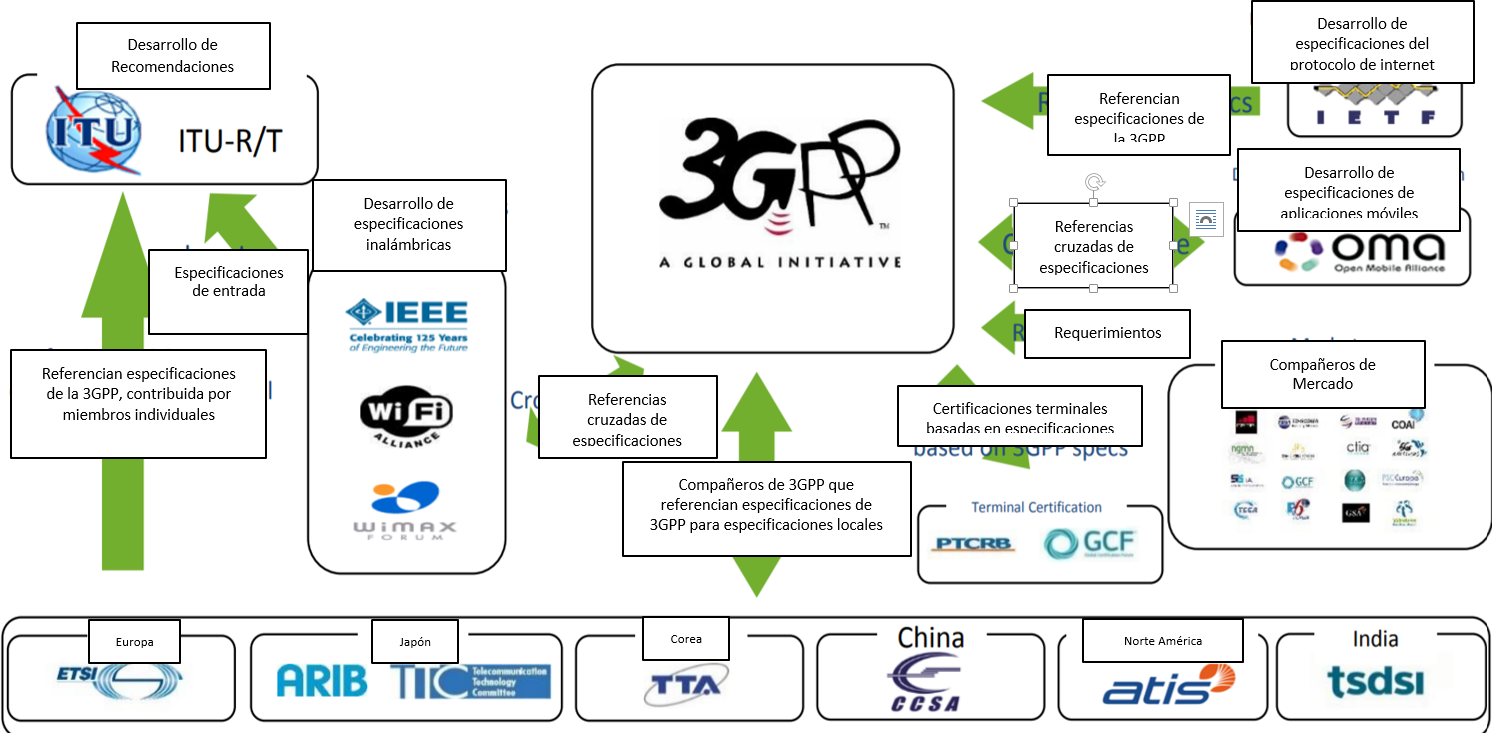
\includegraphics[scale=.5]{Figures/Socios Internacionales con los que colabora la 3GPP}
\decoRule
\caption[Socios Internacionales con los que colabora la 3GPP]{Socios Internacionales con los que colabora la 3GPP, [Fuente: https://www.3gpp.org/about-3gpp/partners]}
\label{fig:socios}
\end{figure}

Además, los socios organizacionales de 3GPP pueden invitar a un socio de representación del mercado a participar en 3GPP, con el fin de ofrecer asesoramiento de mercado a 3GPP y traer a 3GPP una visión consensuada de los requisitos del mercado [\textit{véase Figura~\ref{fig:socios}}].\newline

Los tres grupos de especificaciones técnicas (TSG, \textit{Technical Specifications Group}) de 3GPP,  quienes cada determinado tiempo liberan \textit{releases} (lanzamientos) en los cuales especifican estándares \parencite{3GPP2019}, son:

\begin{enumerate}
\item  Redes de acceso por radio (RAN).
\item  Servicios y aspectos de sistemas (SA).
\item  Red central y terminales (CT).
\end{enumerate} 
% Chapter 3
\chapter{Estado del Arte}
\label{Chapter3} % Change X to a consecutive number; for referencing this chapter elsewhere, use \ref{ChapterX}

En este Capítulo se encuentra el estudio de los trabajos anteriormente realizados que están relacionados con nuestro proyecto terminal, esto con la finalidad de presentar antecedentes, y dejar ver discrepancias y similitudes con el nuestro.\newline

El trabajo de dimensionar los sistemas de comunicación móviles es una necesitad recurrente en cada generación, En \parencite{Celis2016}, se encuentra un proyecto terminal realizado por alumnos de la UPIITA, en el cual se realizó una simulación, bajo el paradigma de eventos discretos, de un sistema celular 4G, con un enfoque en distintos esquemas de reúso de frecuencias y calendarizadores para obtener resultados sobre qué combinación de estos y bajo qué condiciones permitían al sistema tener un mayor desempeño. En este proyecto la simulación se llevó a cabo utilizando Matlab, el paradigma de programación fue el de eventos discretos por lo que presenta un buen precedente a nuestro proyecto.\newline

Por otra parte, el reciente crecimiento de los casos de uso de IoT en una amplia gama de aplicaciones industriales, de servicios públicos y ambientales ha exigido la necesidad de la caracterización del tráfico tipo máquina (MTC). Reconociendo la importancia de este tráfico, la 3GPP ha propuesto dos modelos de tráfico, que modelan el tráfico agregado generado por una gran cantidad de dispositivos. El primero modela el tráfico generado aleatorio, mientras que el segundo modela el tráfico síncrono con el tiempo. Dado que los modelos solo se centran en el tráfico agregado, no son apropiados para el análisis práctico porque no son lo suficientemente precisos como para representar un tráfico M2M real y los modelos no permiten la manipulación máquina por máquina lo que hace difícil para integrar el tráfico en redes celulares.\newline

En \parencite{Gupta2018}, los autores consideraron modelar el tráfico de dispositivos IoT conectados a través de tecnologías LPWAN. Debido a las diversas aplicaciones de IoT, no es trivial tener un solo modelo de tráfico para representarlos a todos, el tráfico puede clasificarse ampliamente como periódico, desencadenado por eventos o una combinación de ambos. Evaluaron el rendimiento de LoRaWAN, en presencia de un híbrido de ambos tipos de tráfico, donde el evento se propaga espacialmente a lo largo del tiempo. Utilizaron el modelo CMMPP para representar dicho tráfico característico de dispositivos IoT independientes activados por un evento. Ya que en una implementación práctica de dispositivos IoT basados en sensores, estos generalmente se implementan densamente para garantizar una medición suficiente y confiable. De este modo, cuando ocurre un evento, exhiben correlación espacial y temporal en su velocidad de tráfico debido a los fenómenos naturales de la métrica que miden. \newline

De igual manera pero ahora con un enfoque en sistemas celulares LTE, en \parencite{Smiljkovic2014} los autores analizaron el tráfico M2M con velocidad de datos variable bajo el supuesto de que la red LTE tiene recursos limitados. Los resultados muestran las características del tráfico M2M de una manera más realista, identificando las diferencias del tráfico estándar en la red celular. Revelan que el tráfico cuenta con la propiedad de auto similitud solo para una gran cantidad de MTC. Además, los resultados dan una idea de los parámetros de diseño que deben considerarse para LTE a fin de admitir el tráfico M2M.\newline

Estos trabajos son una gran aportación ya que demostraron que se puede usar un modelo de tráfico CMMPP para evaluar el impacto en la tecnología de radio IoT, configurando adecuadamente el modelo para representar casos de uso del mundo real. La integración del tráfico M2M en las redes celulares existentes será parte inevitable de la evolución de las redes. En nuestro proyecto se planea evaluar este modelo CMMPP, pero enfocado en sistemas celulares 5G donde se esté dando servicio a usuarios NB-IoT de distintas aplicaciones, además, consideramos un esquema de acceso al medio para la compartición eficiente de los recursos.\newline

Ahora bien, del lado de los esquemas de acceso no ortogonales (NOMA) en redes de quinta generación, y más en concreto de NOMA bajo estándares de 5G/IoT, se ha trabajado arduamente ya que el tema de maximizar la conectividad de los sistemas en escenarios masivos de usuarios esperados en sistemas 5G/IoT son una gran discusión de interés en la actualidad. Dentro de la literatura científica se encuentra toda una gama de propuestas de diferentes modelos de sistema relacionados a NOMA.\newline

En \parencite{Zhang2017}, los autores proponen un sistema usando geometría estocástica (PPP) para modelar un ambiente inalámbrico denso que admita NOMA tanto en el enlace de subida como en el enlace de bajada; el modelado es analítico y validado por simulación. \newline

En la implementación de NOMA proponen dos esquemas de emparejamiento de usuario: uno aleatorio y otro selectivo:
\begin{enumerate}
\item  Cuando el agrupamiento es aleatorio, los UE son seleccionados aleatoriamente.
\item  Cuando el agrupamiento es selectivo, el primer UE deberá tener una relación señal-interferencia más ruido (SINR) por encima del umbral T1 y el segundo UE tiene un SINR por debajo del umbral T2, T2 $\mathrm{\le}$ T1.
\end{enumerate}

Consideraron un error de propagación SIC durante el proceso de decodificación por parte del UE. Además, optaron por una estrategia de asignación de potencia fija, donde la potencia de enlace de bajada asignada a un UE está predefinida y permanece sin cambios.\newline

\begin{figure}
\centering
\begin{minipage}{.45\linewidth}
  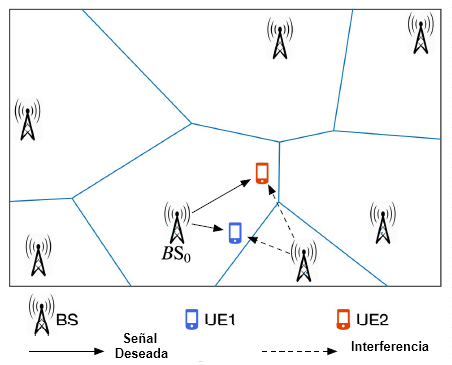
\includegraphics[width=\linewidth]{Modelo de sistema para el sistema de enlace descendente NOMA}
  \captionof{figure}{Modelo de sistema para el sistema de enlace descendente NOMA}
  \label{fig:img1}
\end{minipage}
\hspace{.05\linewidth}
\begin{minipage}{.45\linewidth}
  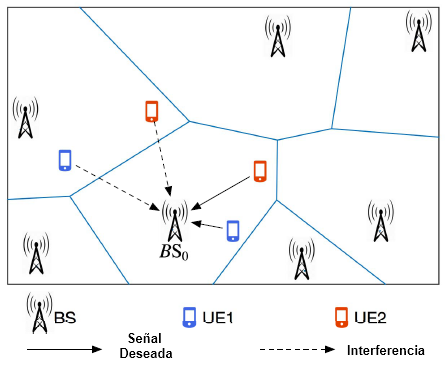
\includegraphics[width=\linewidth]{Modelo de sistema para el sistema de enlace ascendente NOMA}
  \captionof{figure}{Modelo de sistema para el sistema de enlace ascendente NOMA}
  \label{fig:img2}
\end{minipage}
\end{figure}

Las ganancias implementan el desvanecimiento de Rayleigh entre la $BS_0$ y $UE_i$. La ganancia en potencia de desvanecimiento Rayleigh entre BS y UE sigue una distribución exponencial con media 1 y se distribuye de forma independiente e idéntica (i.i.d.)\newline

En el enlace descendente (DL), se agregaron perdidas por trayectoria con un exponente de pérdida y se calcula la interferencia entre celdas cumulativa de todas las bases adyacentes. En el enlace ascendente (UL), la interferencia inter-celdas proviene de todos los otros UEs que comparten la misma sub-banda. \textit{[Véanse Figuras~\ref{fig:img1}, \ref{fig:img2}]}\newline

Como se puede observar, este trabajo se enfocó en NOMA pero para sistemas 5G en general, sin embargo no consideraron la actuación de dispositivos IoT los cuales al tener diferentes calidades de servicio, impactaría en la toma de decisiones con respecto a NOMA, más en concreto en el emparejamiento de usuarios.\newline

Por el contrario, un grupo de autores de la Universidad Británica de Columbia\parencite{Mostafa2019} han trabajado en emplear NOMA para mejorar la densidad de conexión en los sistemas NB-IoT. En su propuesta cada subportadora puede dar servicio máximo a dos dispositivos con diversos requisitos de QoS. \newline

Formularon problemas de asignación de potencia de transmisión y subportadora conjunta para los modos singletone y multitone.  Además, propusieron algoritmos heurísticos con baja complejidad y dieron como resultado un rendimiento cercano a las soluciones óptimas y subóptimas en ambos casos. Los resultados de la simulación mostraron que el uso de NOMA aumentó la densidad de conexión hasta en un 87\% en comparación con OMA en el modo singletone y en el modo multitono, la densidad de conexión también se incrementó hasta en un 24\%.\newline

Los autores en \parencite{Shahini2019} desarrollaron un esquema NOMA en el dominio de potencia con agrupación de usuarios en un sistema NB-IoT. Resolvieron un problema de optimización para maximizar el rendimiento total de la red al optimizar la asignación de recursos de los dispositivos MTC y la agrupación de NOMA al tiempo que satisface los requisitos de potencia de transmisión y QoS. Además, diseñaron un algoritmo heurístico eficiente para resolver el problema de optimización propuesto mediante la optimización conjunta de la agrupación NOMA y la asignación de recursos de dispositivos MTC.\newline

En su modelo de sistema consideraron un escenario de una única celda (solo un eNB), que admite dispositivos MTC basado en el estándar NB-IoT. Asumieron que no hay interferencia entre células de otras células vecinas. \newline

\begin{figure}[th]
\centering
\includegraphics[scale=.6]{Figures/Modelo de sistema de una sola celda usando clusterización}
\decoRule
\caption[Grupos NOMA que incluyen dispositivos mMTC y URLLC, donde los dispositivos MTC comparten los subcanales asignados a cada clúster NOMA.]{Grupos NOMA que incluyen dispositivos mMTC y URLLC, donde los dispositivos MTC comparten los subcanales asignados a cada clúster NOMA.}
\label{fig:NOMA_NBIOT}
\end{figure}

Propusieron un esquema NOMA de dominio de potencia agrupando (de entre 1 a 4) dispositivos mMTC y URLLC en una red NB-IoT como se muestra en la Figura~\ref{fig:NOMA_NBIOT} . Según el esquema NOMA, los dispositivos mMTC y URLLC comparten cada subportadora (subcanal) y transmiten datos de manera no ortogonal, es decir, más de un usuario puede compartir el mismo subcanal. Por lo tanto, los dispositivos se dividen en diferentes grupos, llamados grupos NOMA. Para decodificar con éxito los mensajes del mensaje recibido combinado, el eNB emplea el esquema SIC. Por lo tanto, los usuarios deben ordenarse en cada grupo de acuerdo con el método SIC.\newline

Como vemos, se ha investigado bastante acerca del desempeño de los esquemas NOMA para IoT, sin embargo nuestra propuesta resulta diferente ya que además de considerar un escenario celular bajo un esquema PD-NOMA, se propone implementar un despliegue de UEs usando PPP , porque sirven como modelo de referencia para redes masivas y de interferencia limitada, un modelo de canal más realista y con pérdidas por desvanecimiento rápido, y por último, un modelo de trafico CMMPP que como se ha revisado en \parencite{Gupta2018} son los modelos más realistas para el tráfico MTC.

% Chapter 4

\chapter{Análisis} % Main chapter title


\label{Chapter4} % Change X to a consecutive number; for referencing this chapter elsewhere, use \ref{ChapterX}

En este capítulo se realiza el análisis de las diversas aplicaciones de dispositivos IoT y su implementación en redes de comunicaciones móviles 5G. Se comienza con una breve descripción de estas tecnologías, y después se profundiza en el caso de uso mMTC donde se mencionan los escenarios más comunes de implementación, su clasificación y sus características, además se revisa el estándar actual (NB-IoT\footnote{ Muchos\ de\ los\ modelos\ aqu\textrm{í}\ propuestos\ est\textrm{á}n\ basados\ en\ trabajos\ de\ la\ 3GPP,\ como\ se\ revis\textrm{ó}\ en\ el Capítulo \ref{Chapter2},\ la\ 3GPP,\ es\ una\ organizaci\textrm{ó}n\ que\ est\textrm{á}\ respaldada\ por\ organismos\ alrededor\ de\ todo\ el\ mundo,\ adem\textrm{á}s\ de\ que\ se\ trata\ del\ grupo\ que\ estandariza\ tecnolog\textrm{í}as\ como\ LTE-M\ y\ NB-IoT,\ de\ manera\ que\ es\ una\ indudable\ referencia\ en\ su\ ahora\ inmersi\textrm{ó}n\ en\ la\ estandarizaci\textrm{ó}n\ de\ 5G.}) que cumple con los requisitos para la implementación de mMTC. Finalmente también se revisan los KPIs propuestos para este tipo de escenarios.\newline

Por último, se detallan cuáles son los modelos y técnicas que se usan para caracterizar el modelo de despliegue, canal y de tráfico de dispositivos IoT en redes 5G y además se presenta la actual propuesta de técnica de acceso múltiple al medio no ortogonal (NOMA) y su enfoque hacia un entorno masivo de dispositivos (con el uso de \textit{clusterización}).

%----------------------------------------------------------------------------------------
%	SECTION 
%----------------------------------------------------------------------------------------

\section{REDES 5G/IoT}

Aunque gran parte de la comunicación IoT se ha implementado hasta el momento, no se ha considerado para una conectividad masiva y una mejor eficiencia energética. \newline

IoT en los sistemas 5G tendrán un importante papel en esta generación futura ya que abrirán una puerta para una nueva arquitectura inalámbrica y servicios inteligentes. La reciente red celular LTE (4G) no será lo suficientemente eficiente para satisfacer las demandas de conectividad de múltiples dispositivos y velocidad de datos, calidad de servicio (QoS) de baja latencia y baja interferencia. Para abordar estos desafíos, 5G es la tecnología más prometedora \parencite{Chetri2020}. \newline

Por lo tanto, la comunicación masiva de tipo máquina (mMTC), será uno de los principales habilitadores clave para el despliegue de redes 5G-IoT.

%----------------------------------------------------------------------------------------
%	SECTION 
%----------------------------------------------------------------------------------------

\section{CLASIFICACIÓN Y ANÁLISIS DE LOS ÁMBITOS DE IoT}

La contribución en cuanto a la categorización de las aplicaciones de IoT que ya existen y las que se comenzarán a ver en años próximos, es vasta y no siempre compatible dependiendo del grupo que se consulte, de manera que se tomó como referencia el trabajo realizado en \parencite{NetTrafficIoT} como guía para los servicios que se espera brinden los nodos IoT en distintos ámbitos.\newline

La mayor parte del artículo \parencite{NetTrafficIoT}, los autores se dedicaron a la caracterización de las aplicaciones de IoT y sus dominios, los cuales se pueden dividir en 8, específicamente: edificios inteligentes y vivienda (\textit{Smart buildings and living}), cuidado de la salud inteligente (\textit{Smart healthcare}), medio ambiente inteligente (\textit{Smart environment}), ciudades inteligentes (\textit{Smart city}), energía inteligente (\textit{Smart energy}), transporte y movilidad  inteligentes (\textit{Smart transport and mobility}), fabricación y venta inteligentes (\textit{Smart manufacturing and retail}), agricultura inteligente (\textit{Smart agriculture}). Para cada uno de los dominios se especifican aplicaciones típicas que se podrían encontrar, sus características de tráfico, las tecnologías de red más adecuadas para darles servicio entre otras cosas.\newline

La primera parte del análisis correspondió a la selección de los dominios que resultasen adecuados para el sistema que se diseña, es decir los dominios cuya red que les brindará servicio primordialmente será una red de área amplia de bajo consumo (LPWAN, \textit{Low Power Wide Area Network}). Esto se debe a que algunas de las aplicaciones en los dominios antes mencionados están pensadas para redes de distintas características en las que tecnologías como RFID, \textit{Bluetooth }o \textit{ZigBee }podrían ser una mejor solución. A continuación se presenta la caracterización de cada uno de los dominios que en \parencite{NetTrafficIoT} se consideran viables para redes LPWAN.\newline

\subsection{Ciudades inteligentes \textit{(Smart City)}:}

Con el rápido incremento de la población y su concentración en poblaciones urbanas, se ha convertido en una prioridad la reducción del uso de recursos públicos, así como la reducción de costos de operación del día a día de una ciudad, ambas de la manera más óptima posible. Las aplicaciones en este dominio tratan justamente de abordar estos problemas y los servicios que brindan son bastante variados, los ejemplos van desde el control de luminarias hasta el manejo de desechos, estos y otros  pueden encontrarse en la \textit{Tabla~\ref{tab:smartcity}}, acompañados de más información tal como la caracterización de su tráfico y su demanda de QoS.\newline

\begin{table}
\caption{Características de las aplicaciones de Ciudades Inteligentes}
\label{tab:smartcity}
\centering
\begin{tabular}{*{5}{m{3cm}}}\\
\textbf{\textit{Servicio}} & \textbf{\textit{Tamaño de red}} & \textbf{\textit{Tasa de tráfico}} & \textbf{\textit{Demanda de QoS}} & \textbf{\textit{Fuente de energía}} \\ \hline \hline
\textit{Monitoreo del consumo de agua y electricidad en la ciudad} & \footnotesize{Media a grande, cientos a miles de dispositivos} & \footnotesize{Periódico, 1 msj cada 10 min por dispositivo} & \footnotesize{Baja, tolerante al retardo 1 min} & \footnotesize{Alimentado por la red eléctrica/ autoalimentado} \\ \hline
\textit{Control de iluminación} & \footnotesize{Grande, miles de dispositivos} & \footnotesize{Aleatorio, poco frecuente} & \footnotesize{Media, tolerante al retardo 15 seg} & \footnotesize{Alimentado por la red eléctrica }\\ \hline
\textit{Vigilancia de estacionamientos} & \footnotesize{Grande, miles de dispositivos} & \footnotesize{Aleatorio, poco frecuente} & \footnotesize{Media, tolerante al retardo 10 seg} & \footnotesize{Alimentado por batería }\\ \hline
\textit{Control del tráfico} & \footnotesize{Grande, miles de dispositivos} & \footnotesize{Periódico, 1 msj cada 10 min por dispositivo, aleatorio para alarmas} & \footnotesize{Media, tolerante al retardo 15 seg, alta para alarmas} & \footnotesize{Alimentado por batería} \\ \hline
\textit{Mantenimiento de deshechos} & \footnotesize{Grande, miles de dispositivos} & \footnotesize{Aleatorio, poco frecuente} & \footnotesize{Media, tolerante al retardo 30 seg} & \footnotesize{Alimentado por batería }\\ \hline
\textit{Monitoreo de condiciones urbanas} & \footnotesize{Media a grande, cientos a miles de dispositivos} & \footnotesize{Periódico, 1 msj cada 15 min por dispositivo, aleatorio para alarmas} & \footnotesize{Media, tolerante al retardo 30 seg, alta para alarmas} & \footnotesize{Alimentado por batería }\\ \hline
\textit{Monitoreo de la salud estructural de edificios} & \footnotesize{Media a grande, cientos a miles de dispositivos} & \footnotesize{Periódico, 1 msj cada 15 min por dispositivo, aleatorio para alarmas} & \footnotesize{Media, tolerante al retardo 30 seg, alta para alarmas} & \footnotesize{Alimentado por batería} \\ 
\end{tabular}
\end{table}

\subsection{Ambiente inteligente \textit{(Smart Environment)}}

Este dominio comprende las aplicaciones que se encargan de monitorear el ambiente a nuestro alrededor y lo que ocurre en él, y aunque no se pueda controlar la fuerza de la naturaleza, con una correcta observación se pueden detectar distintos fenómenos naturales y reaccionar a tiempo ante ellos. En el caso especial de eventos que podrían ocasionar una catástrofe, es importante reaccionar lo más rápido posible por lo que el brindar el servicio a algunas de las aplicaciones de este dominio se volverá crítico. En la \textit{Tabla~\ref{tab:smartenv}} podemos encontrar la caracterización de las aplicaciones consideradas en \parencite{NetTrafficIoT} para \textit{Ambiente Inteligente.}\newline


\begin{table}
\caption{Características de las aplicaciones de Ambiente Inteligente}
\label{tab:smartenv}
\centering
\begin{tabular}{*{5}{m{3cm}}} \\ 
\textbf{\textit{Servicio}} & \textbf{Tamaño de red} & \textbf{Tasa de tráfico} & \textbf{Demanda de QoS} & \textbf{Fuente de energía} \\ \hline 
\textit{Detección de incendios forestales}  & \footnotesize{ Media a grande, cientos a miles de dispositivos } & \footnotesize{ Aleatorio, poco frecuente } & \footnotesize{ Media, tolerante al retardo 15 seg } & \footnotesize{ Alimentado por batería } \\ \hline 
\textit{Detección de terremotos}  & \footnotesize{ Media a grande, cientos a miles de dispositivos } & \footnotesize{ Aleatorio, poco frecuente } & \footnotesize{ Alta, tolerante al retardo 5 seg } & \footnotesize{ Alimentado por batería } \\ \hline 
\textit{Detección de Tsunamis}  & \footnotesize{ Media a grande, cientos a miles de dispositivos } & \footnotesize{ Aleatorio, poco frecuente } & \footnotesize{ Alta, tolerante al retardo 5 seg } & \footnotesize{ Alimentado por batería } \\ \hline 
\textit{Detección de derrumbes y avalanchas}  & \footnotesize{ Media a grande, cientos a miles de dispositivos } & \footnotesize{ Aleatorio, poco frecuente } & \footnotesize{ Alta, tolerante al retardo 5 seg } & \footnotesize{ Alimentado por batería } \\ \hline 
\textit{Monitoreo de actividad volcánica}  & \footnotesize{ Pequeña, 10s de dispositivos } & \footnotesize{ Aleatorio, poco frecuente } & \footnotesize{ Alta, tolerante al retardo 5 seg } & \footnotesize{ Alimentado por batería } \\ \hline 
\textit{Monitoreo de la contaminación del aire } & \footnotesize{ Media a grande, cientos a miles de dispositivos } & \footnotesize{ Periódico, 1 msj cada 15 min por dispositivo } & \footnotesize{ Media, tolerante al retardo 15 seg } & \footnotesize{ Alimentado por batería } \\ \hline 
\textit{Rastreo de vida salvaje.}  & \footnotesize{ Media, cientos de dispositivos } & \footnotesize{ Periódico, 1 msj cada 30 min por dispositivo } & \footnotesize{ Baja, tolerante a unas horas } & \footnotesize{ Alimentado por batería } \\ 
\end{tabular}
\end{table}

\subsection{Energía inteligente \textit{(Smart Energy)}:}

El dominio de Energía Inteligente\textit{Smart Energy }se refiere a las mejoras en la distribución y el consumo de fuentes de energía o recursos necesarios, tales como la electricidad, el gas y el agua. Aunque el foco de atención está en la electricidad ya que existe una tendencia más marcada hacia su ahorro y la utilización de fuentes renovables. \newline

Los nodos de IoT para aplicaciones de este dominio podrían monitorear las condiciones cambiantes de la red, para posteriormente generar una reconfiguración apropiada del servicio. En la \textit{Tabla~\ref{tab:smartenergy}} podemos encontrar la caracterización descrita en \parencite{NetTrafficIoT} para distintas aplicaciones de Energía Inteligente.\newline

\begin{table}
\caption{Características de las aplicaciones de Energía Inteligente}
\label{tab:smartenergy}
\centering


\begin{tabular}{*{5}{m{3cm}}}  \\  
\textbf{\textit{Servicio}} & \textbf{Tamaño de red} & \textbf{Tasa de tráfico} & \textbf{Demanda de QoS} & \textbf{Fuente de energía} \\ \hline
\textit{Medición inteligente}  & \footnotesize{ Media a grande, 1 dispositivo por hogar } & \footnotesize{ Periódico, 1 msj cada 15 min por dispositivo } & \footnotesize{ Media, tolerante al retardo 15 seg } & \footnotesize{ Alimentado por la red eléctrica/ Baterías } \\ \hline 
\textit{Gestión de activos}  & \footnotesize{ Media a grande, cientos a miles de dispositivos } & \footnotesize{ Periódico, 1 msj cada 15 min por dispositivo } & \footnotesize{ Media, tolerante al retardo 15 seg } & \footnotesize{ Alimentado por la red eléctrica/ Baterías } \\ \hline 
\textit{Detección de interrupciones en el servicio } & \footnotesize{ Media a grande, 1 dispositivo por hogar } & \footnotesize{ Aleatorio, poco frecuente } & \footnotesize{ Alta, tiempo real } & \footnotesize{ Alimentado por la red eléctrica/ Baterías } \\ 
\end{tabular}
\end{table}

\subsection{Transporte y movilidad inteligentes \textit{(Smart Transport and Mobility)}:}

Tanto el crecimiento urbano como el crecimiento de las fuentes de transporte de pasajeros y de mercancías, con más frecuentes congestiones viales y una mayor movilidad requerida, han creado una demanda de administrar el transporte y la movilidad de una manera más inteligente. \newline

El objetivo de aplicaciones IoT en el dominio de Transporte y movilidad inteligentes\textit{ (Smart Transport and Mobility)}es ayudar a resolver el problema de movilidad tanto de pasajeros como de mercancías, haciéndolo más rápido, más barato y más seguro. En la \textit{Tabla~\ref{tab:smartrans}} se encuentra la caracterización presentada en \parencite{NetTrafficIoT} para distintas aplicaciones de este dominio.\newline

\begin{table}
\caption{Características de las aplicaciones de Transporte y Movilidad inteligentes}
\label{tab:smartrans}
\centering
\begin{tabular}{*{5}{m{3cm}}}\\ 
\textit{Servicio} & Tamaño de red & Tasa de tráfico & Demanda de QoS & Fuente de energía \\ \hline
\textit{Automatización de vehículos}  & \footnotesize{ Grande, miles de dispositivos } & \footnotesize{ Periódico, 1 msj cada 24 hrs por vehículo. } & \footnotesize{ Baja, tolerante al retardo 1 min } & \footnotesize{ Alimentado por batería del vehículo } \\ \hline 
\textit{Localización y monitoreo de vehículos}  & \footnotesize{ Grande, miles de dispositivos } & \footnotesize{ Periódico, 1 msj cada 30 seg por vehículo } & \footnotesize{ Media, tolerante al retardo 10 seg } & \footnotesize{ Alimentado por batería del vehículo } \\ \hline 
\textit{Monitoreo de la calidad del embarque}  & \footnotesize{ Media, cientos de dispositivos } & \footnotesize{ Periódico, 1 msj cada 15 min por dispositivo } & \footnotesize{ Media, tolerante al retardo 15 seg } & \footnotesize{ Alimentado por batería } \\ \hline 
\textit{Control dinámico de semáforos}  & \footnotesize{ Grande, miles de dispositivos } & \footnotesize{ Periódico, 1 msj cada min por dispositivo } & \footnotesize{ Alta, tolerante al retardo 5 seg } & \footnotesize{ Alimentado por la red eléctrica } \\ \hline 
\textit{Monitoreo de las condiciones del camino} & \footnotesize{ Grande, miles de dispositivos } & \footnotesize{ Aleatorio, poco frecuente } & \footnotesize{ Media, tolerante al retardo 30 seg } & \footnotesize{ Alimentado por batería } \\
\end{tabular}
\end{table}

%----------------------------------------------------------------------------------------
%	SECTION 
%----------------------------------------------------------------------------------------

\section{CARACTERÍSTICAS DEL ESCENARIO A IMPLEMENTAR}

Las distintas aplicaciones presentadas en la sección anterior pertenecen a varios dominios y estas muy seguramente se verán desplegadas en un futuro próximo en ciudades alrededor de todo el mundo. Una aserción que resulta importante es la gran cantidad de aplicaciones que se esperan para IoT \parencite{Ericsson2019}, pero en este análisis se toman en consideración únicamente aquellas bajo el paradigma de redes LPWAN, para las cuales la red celular podría ser las más idónea para brindarles servicio. En estas aplicaciones lo primordial es tener un bajo consumo y complejidad de los dispositivos, además de una amplia cobertura y una gran densidad de dispositivos \parencite{5GAmericas}, en contraste con las aplicaciones más inclinadas a los casos de uso eMBB y URLLC donde lo primordial es el amplio ancho de banda disponible para las aplicaciones y una menor latencia, respectivamente.\newline

\subsection{Análisis de las aplicaciones de IoT y selección de casos considerados}

De todos los servicios descritos en las tablas anteriores \textit{[Tabla~\ref{tab:smartcity}\ldots \ref{tab:smartrans}]}, se ha decidido simular solamente un grupo diverso de aplicaciones provenientes de distintos dominios. Este grupo se seleccionó a manera que fuera representativo de distintos comportamientos y requerimientos de QoS. El escenario propuesto consta de los servicios de: control de iluminación, monitoreo del consumo de agua y electricidad, detección de terremotos, monitoreo de contaminación del aire, detección de interrupciones en el servicio (agua, luz, gas), control dinámico de semáforos y un último servicio que se llamó ``genérico''. El servicio llamado genérico representará el conglomerado de todas las demás aplicaciones IoT que estarán presentes en la red y no corresponden a una de estas aplicaciones. \newline

Se decidió entonces situar la simulación en un escenario urbano micro celular con nodos en exteriores, en el que se encontrarán todas las aplicaciones mencionadas en el párrafo anterior. La elección de un escenario urbano micro celular se debe a que en este se puede experimentar la congestión de las comunicaciones MTC y HTC, ya que corresponde a zonas urbanas densamente pobladas. Otra razón es que en un escenario tal se tienen presentes una mayor diversidad de aplicaciones IoT, con distintas características de tráfico y requerimientos de QoS. La densidad de dispositivos aunado a su diversidad ayudará a que la simulación contemple comportamientos reales y seamos capaces de evaluar los KPIs deseados.\newline

En la \textit{Tabla~\ref{tab:appssim}} se presentan las aplicaciones IoT del escenario urbano que se determinaron y como se puede apreciar, se seleccionaron aplicaciones provenientes de distintos dominios para tener cierta variedad, pero más importante que eso es la diversidad en las características del tráfico generado y en los parámetros de QoS requeridos por cada una de estas aplicaciones. \newline

A continuación se hace una descripción de la \textit{Tabla~\ref{tab:appssim}}. Se tienen tres aplicaciones con una alta demanda de QoS, después dos con una demanda media y finalmente una demanda baja, las distintas demandas de QoS se traducen en diferentes tolerancias a la latencia, las cuales van desde los minutos hasta aquellas que requieren de una respuesta casi inmediata. Es importante aclarar que el término ``tiempo real'' se arrastra de la descripción dada en \parencite{NetTrafficIoT}, la cual en el contexto de nodos IoT dependerá dependiendo del caso de uso de estos, es decir, la consideración de tiempo real no es la misma para aplicaciones URLLC que para aplicaciones mMTC. Otra caracterización que se consideró para decidir entre las aplicaciones fue la tasa de tráfico de estas, se trató entonces de tener nodos con distintos periodos de transmisión, por ejemplo el servicio que brindarán nodos monitoreando la contaminación del aire tendrá un periodo de 15 minutos mientras que el de nodos controlando los semáforos será de 1 minuto. Por otro lado hay también nodos con tasas de trasmisión aleatorias como el caso del de detección de terremotos. \newline

La decisión de agregar un servicio más que fuera genérico surge a raíz de la necesidad de representar en la red los dispositivos restantes con comportamientos de lo más diversos, razón por la cual se consideró que este tendrá una tasa de tráfico aleatoria y su requerimiento de QoS será superior al de la mayoría.\newline

Finalmente se introduce una distinción entre nodos que se mencionará principalmente en el capítulo~\ref{Chapter5}, se trata de la clasificación de dispositivos de Clase 1 y de Clase 2, esta distinción está ligada directamente a la aplicación del noto IoT que determina a su vez la demanda de QoS. Los nodos con mayores requerimientos de QoS que son a su vez la minoría del total de dispositivos corresponden a la clase 2, mientras que todo el resto de nodos corresponden a la clase 1. En la \textit{Tabla~\ref{tab:appssim}}los nodos que dicen requerir de una transmisión en tiempo real corresponderán entonces a aquellos de clase 2.\newline


\begin{table}
\caption{Aplicaciones seleccionadas para la simulación}
\label{tab:appssim}
\centering
\begin{tabular}{*{5}{m{3cm}}} \\ 
\textbf{\textit{Servicio}} & \textbf{Tamaño de red} & \textbf{Tasa de tráfico} & \textbf{Demanda de QoS} & \textbf{Fuente de energía} \\ 
\textit{Control de iluminación (Ciudad Inteligente)}  & \footnotesize{ Grande, miles de dispositivos } & \footnotesize{ Aleatorio, poco frecuente } & \footnotesize{ Media, tolerante al retardo 15seg } & \footnotesize{ Alimentado por la red eléctrica } \\ \hline 
\textit{Monitoreo del consumo de agua y electricidad en la ciudad (Ciudad Inteligente)}  & \footnotesize{ Media a grande, cientos a miles de dispositivos } & \footnotesize{ Periódico, 1 msj cada 10 min por dispositivo } & \footnotesize{ Baja, tolerante al retardo 1min } & \footnotesize{ Alimentado por la red eléctrica/ autoalimentado } \\ \hline 
\textit{Detección de terremotos (Ambiente Inteligente)}  & \footnotesize{ Media a grande, cientos a miles de dispositivos } & \footnotesize{ Aleatorio, poco frecuente } & \footnotesize{ Alta, tolerante al retardo 3seg } & \footnotesize{ Alimentado por batería } \\ \hline 
\textit{Monitoreo de contaminación del aire (Ambiente Inteligente) } & \footnotesize{ Media a grande, cientos a miles de dispositivos } & \footnotesize{ Periódico, 1 msj cada 15 min por dispositivo } & \footnotesize{ Media, tolerante al retardo 15seg } & \footnotesize{ Alimentado por batería } \\ \hline 
\textit{Control dinámico de semáforos (Transporte y Movilidad Inteligentes)} & \footnotesize{ Grande, miles de dispositivos } & \footnotesize{ Periódico, 1 msj cada min por dispositivo } & \footnotesize{ Alta, tolerante al retardo 5seg } & \footnotesize{ Alimentado por la red } \\ \hline 
\textit{Genérico}  & \footnotesize{ Grande, miles de dispositivos } & \footnotesize{ Aleatorio, poco frecuente } & \footnotesize{ Alta, tiempo real } & \footnotesize{ Alimentado por batería } \\ 
\end{tabular}
\end{table}

La distinción entre clases 1 y 2 será útil a la hora de implementar la tecnología de acceso múltiple, pues diversos nodos pertenecerán al mismo grupo y compartirán recursos, de manera que será necesario que exista una jerarquía entre ellos, todo esto será explicado en el diseño.

\subsection{Análisis de las tecnologías para IoT y selección de casos considerados}

NB-IoT y LTE-M (\textit{LTE for MTC}) son dos tecnologías LPWA desarrolladas para aplicaciones IoT. Ambas son protocolos para comunicaciones celulares con un ancho de banda bajo que conectan a internet dispositivos que necesitan transmitir pequeñas cantidades de datos, a bajo coste (tanto en lo relativo al hardware como a la suscripción) y con una alta duración de la batería.\newline

Para ser muy específicos, LTE-M y NB-IoT son las dos categorías de nivel superior de dispositivos de baja potencia y bajo ancho de banda explicados por el 3GPP. Dentro de cada uno hay subtipos y subtipos, muy necesarios para una mayor especialización en el estándar 3GPP. \newline

Debido a la espera que NB-IoT y LTE-M cumplan con los requerimientos LPWAN del estándar 5G, 3GPP ha indicado a ITU-R que ambas tecnologías serán propuestas para el estándar, coexistiendo con los demás componentes de la red que en conjunto cumplirán con la QoS de todos los distintos casos de uso de la red 5G. De manera que esto convierte a NB-IoT y LTE-M como parte de 5G \parencite{EricssonAB2016}. \newline

Las redes de largo alcance LPWAN utilizan tecnología capaz de transferir mensajes a decenas de kilómetros de distancia y cubrir una amplia área. Son redes especializadas en interconectar dispositivos en ambientes restringidos, de difícil acceso o que simplemente buscan reducir el consumo de energía en estos, manteniendo un bajo costo y complejidad. Por lo tanto concentran en un eficiente consumo de la energía y una cobertura amplia \parencite{NetTrafficIoT}, (que se acopla bastante bien a lo que se requieren los nodos de IoT de las aplicaciones seleccionadas en la sección anterior). \newline

A continuación se presentan las tecnologías de red actuales para nodos de IoT en redes móviles, especificadas por la 3GPP, que formarán parte también de las especificaciones de 5G:
\begin{enumerate}
    \item \textit{\underbar{eMTC (enhanced Machine Type Communication:)}} Forma parte de la familia LTE-M y es una evolución de LTE optimizada para IoT. Se desarrolló con el objetivo de una eficiencia energética.
    \item \textit{\underbar{NB-IoT (Narrow-Band Internet of Things:)}} fue estandarizado en el \textit{release }13 de 3GPP y se espera que consiga dar servicio a más dispositivos con energía limitada que eMTC. NB-IoT no requiere ningún desarrollo adicional de redes ya que se implementa en funcionalidades ya existentes de LTE \parencite{NetTrafficIoT} y en un futuro será implementado directamente en la banda de frecuencias de 5G NR [\textit{véase Figura~\ref{fig:5gnr}}] \parencite{EricssonAB2016}.
\end{enumerate}

IoT masivo (mIoT) incluye principalmente áreas amplias que conectan grandes números de dispositivos, objetos y maquinas ya sean estáticos o móviles de baja complejidad y bajo costo con una batería de larga duración y un rendimiento relativamente bajo. \newline

El soporte para mIoT ya se brinda en las redes LTE de hoy con NB-IoT y eMTC. Estas tecnologías se complementan entre sí y existe una tendencia emergente hacia los proveedores de servicios que implementan una red común que admita ambas tecnologías.\newline

eMTC es adecuado para usar casos que requieren un rendimiento relativamente más alto, una latencia más baja y soporte de voz, mientras que la tecnología NB-IoT es conveniente para casos de uso bajo que toleran demoras pero requieren una cobertura extendida, además de que presenta una mejor cobertura en interiores \parencite{EricssonAB2016}. \newline

Según \parencite{Ericsson2019} a finales de 2024, se espera que NB-IoT y eMTC representen cerca del 45 por ciento de todas las conexiones CIoT (\textit{Celullar IoT}). Además, en el futuro NB-IoT y eMTC podrán coexistir completamente en bandas de espectro con 5G NR, \textit{Figura~\ref{fig:5gnr}}.\newline

\begin{figure}[th]
\centering
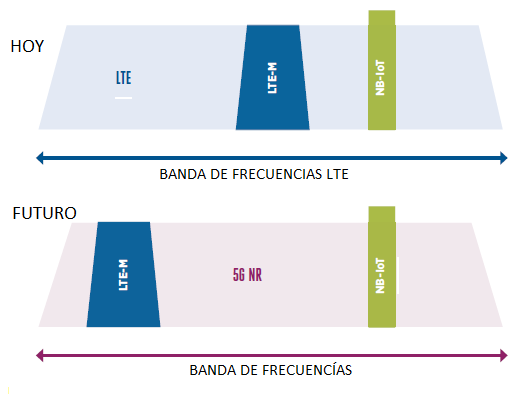
\includegraphics[scale=1]{Figures/5G NR con LTE-M y NB-IoT en banda}
\decoRule
\caption[5G NR con LTE-M y NB-IoT en banda]{5G NR con LTE-M y NB-IoT en banda}
\label{fig:5gnr}
\end{figure}

En la \textit{Tabla~\ref{tab:tecIoT}} se pueden encontrar características de estas tecnologías antes descritas, tales como la banda de frecuencia a la que operan y su tasa de transmisión y si bien pareciera que la diferencia entre ambas tecnologías es sutil, en realidad, ésta marca una clara pauta en el servicio que pueden brindar. \newline

\begin{table}
\caption{Características de las tecnologías de red para IoT en la red celular}
\label{tab:tecIoT}
\centering
\begin{tabular}{|p{0.6in}|p{0.6in}|p{0.4in}|p{0.6in}|p{0.4in}|p{0.5in}|p{0.8in}|p{0.4in}|} \\ 
\textbf{\textit{Tecnología}} & \textbf{\textit{Banda de Frecuencia}} & \textbf{\textit{Rango}} & \textbf{\textit{Tasa de transmisión}} & \textbf{\textit{Vida de la batería}} & \textbf{\textit{Topología}} & \textbf{\textit{Estandarización}} & \textbf{\textit{Grupo}} \\ 
\textbf{NB-IoT}  & \footnotesize{ 450 MHZ -- 3.5 GHz (Espectro de 2G/3G/4G) } & \footnotesize{ 10-15 km } & \footnotesize{ 250 kbps } & \footnotesize{ 10+ años } & \footnotesize{ Estrella } & \footnotesize{ Abierto } & \footnotesize{ 3GPP } \\ \hline
\textbf{eMTC}  & \footnotesize{ 450 MHZ -- 3.5 GHz (El mismo que LTE) } & \footnotesize{ 10-15 km } & \footnotesize{ 1 Mbps } & \footnotesize{ 10+ años } & \footnotesize{ Estrella } & \footnotesize{ Abierto } & \footnotesize{ 3GPP } \\
\end{tabular}

\end{table}


En la \textit{Figura~\ref{fig:lpwa}} se puede observar otra comparación entre ambas tecnologías pero en esta ocasión desde la perspectiva de las aplicaciones a la que tanto NB-IoT y/o LTE-M estarían dando servicio preferentemente. A la izquierda de la \textit{Figura~\ref{fig:lpwa}} tenemos las aplicaciones LPWAN a las que NB-IoT daría servicio que coinciden con una menor velocidad de transferencia y mayor tolerancia a la latencia mientras que a la derecha se aglomeran las aplicaciones que requieren una comunicación en tiempo real y una mayor tasa de transmisión, aplicaciones a las que estaría dando servicio preferentemente la tecnología eMTC. \newline

Se decidió entonces concentrarse en la tecnología NB-IoT puesto que la totalidad de los servicios que se considerarán en nuestro sistema pueden situarse a la izquierda de la \textit{Figura~\ref{fig:lpwa}}, donde se presenta una mínima movilidad de los dispositivos, por ejemplo el control de la iluminación y el control dinámico de los semáforos podríamos colocarlos en \textit{Iluminación pública y Ciudades inteligentes }respectivamente, mientras que el monitoreo de consumo energético y el de la condición del aire podrían corresponder a \textit{Medidores inteligentes}, de manera que quizá el único servicio que se encontraría en los límites de la tecnología NB-IoT sería el de detección de cortes en el suministro energético, el cual en \parencite{NetTrafficIoT} establece que requeriría de una mínima latencia.\newline


\begin{figure}[th]
\centering
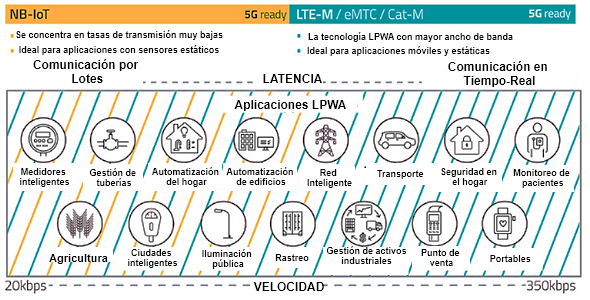
\includegraphics[scale=1]{Tecnología líder para el caso de uso LPWA}
\decoRule
\caption[Tecnologías líder para el caso de uso LPWA]{Tecnologías líder para el caso de uso LPWA, [Fuente: https://www.iotforall.com/cellular-iot-explained-nb-iot-vs-lte-m/]}
\label{fig:lpwa}
\end{figure}

Con esta argumentación se explica la decisión de haber seleccionado la tecnología de red NB-IoT como de la que partiremos para después agregar mejoras propuestas en otros trabajos y diseñar un modelo de sistema para la simulación en el que con modelos de tráfico adecuados se puedan medir los indicadores clave de rendimiento y determinar si la calidad de servicio esperada para los servicios LPWAN seleccionados se cumplirán en redes celulares 5G.

La \textit{Figura~\ref{fig:5gqos}} muestra las distintas tecnologías con las que estaría trabando 5G NR para poder brindar servicio al amplio espectro de casos de uso de MTC \parencite{5GAmericas}. La tecnología NB-IoT podemos situarla en las frecuencias de operación baja y con un una tolerancia al retardo mayor que la mayoría de las demás tecnologías.

\begin{figure}[th]
\centering
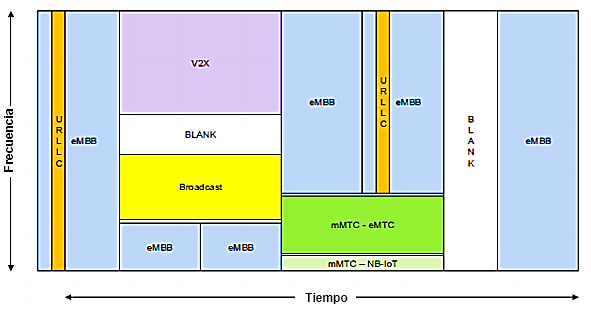
\includegraphics[scale=1]{5G NR soportará múltiples servicios con distintos requerimiento de QoS}
\decoRule
\caption[5G NR soportará múltiples servicios con distintos requerimiento de QoS]{5G NR soportará múltiples servicios con distintos requerimiento de QoS}
\label{fig:5gqos}
\end{figure}

\subsection{Análisis del estándar NB-IoT} \label{NBIoT}

En particular, el estándar NB-IoT fue especificado en el reporte TR 45.820 (\textit{release} 13) de la 3GPP \parencite{3GPP2019}. Los parámetros fundamentales son:\newline

Para el enlace de subida (\textit{uplink}), como su nombre lo indica, tiene un ancho de banda estrecho de 180 kHz y un espacio de sub-portadora de 3.75 kHz (ancho de banda de transmisión mínimo para un dispositivo). Por lo tanto puede asignar 48 sub-portadoras [\textit{véase Figura~\ref{fig:NBIoT}}].

\begin{figure}[th]
\centering
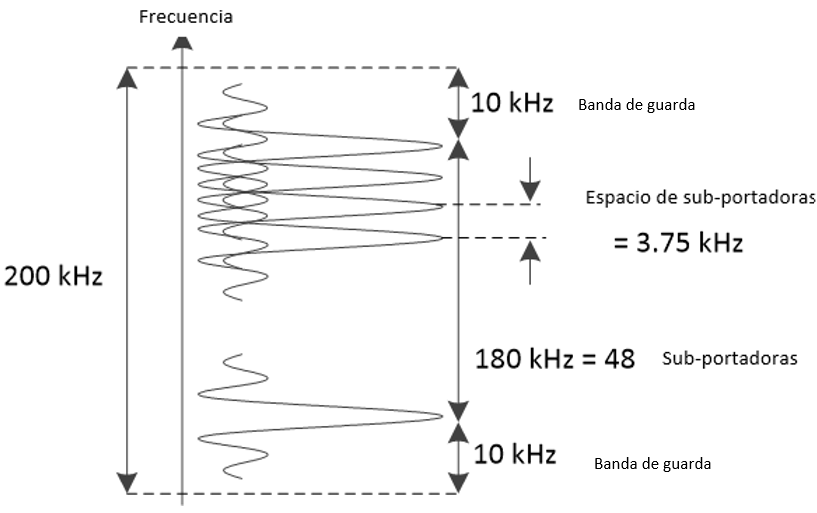
\includegraphics[scale=1]{Estructura de ancho de banda y subportadoras en NB-IoT}
\decoRule
\caption[Estructura de ancho de banda y subportadoras en NB-IoT.]{Estructura de ancho de banda y subportadoras en NB-IoT.}
\label{fig:NBIoT}
\end{figure}

El enlace de bajada (\textit{downlink}), se conserva la estructura de transmisión del enlace descendente de \textit{Long Term Evolution} (LTE) con un espaciado de sub-portadora de 15 kHz.\newline

Por lo tanto, NB-IoT puede proporcionar velocidades de datos de casi 250 kb / s en el enlace descendente y 20 kb / s en el enlace ascendente.\newline

Es preciso puntualizar que para lograr una mayor tasa de datos, de acuerdo con el Teorema de Shannon-Hartley (Ecuación~\ref{eqn:Shannon}), el ancho de banda debe ser elevado o una relación S/N alta. Para el caso de NB-IoT se cuenta con un ancho de banda muy pequeño (3.75KHz), por lo cual alcanzar una buena relación S/N (en este caso, para sistemas celulares S/I) es de suma importancia.\\

La tecnología NB-IoT al ocupar un ancho de banda de frecuencias de 180 kHz, corresponde a un bloque de recursos en la transmisión LTE. \newline

Modos de operación\parencite{Liberg2018}:

Independiente (stand-alone).\newline

NB-IoT puede implementarse como una portadora autónoma utilizando cualquier espectro disponible con un ancho de banda superior a 180 kHz. Esto se conoce como la implementación stand-alone. Un caso de uso de este despliegue autónomo es que un operador GSM despliegue NB-IoT en su banda GSM reajustando parte de su espectro GSM.\newline

Despliegue en banda (in-band) y en guarda de banda (guard-band) LTE.\newline

NB-IoT también está diseñado para su despliegue en las redes LTE existentes, ya sea utilizando uno de los bloques de recursos físicos (PRB) de LTE o utilizando la banda de guarda LTE. El despliegue en banda de guarda hace uso del hecho de que el ancho de banda ocupado en LTE es aproximadamente el $90\%$ del ancho de banda del canal\newline

Para el modo de operación independiente y de banda de guarda, el PRB de enlace descendente y ascendente debe establecerse simétricamente y para el modo en banda, el despliegue del PRB estará restringido a algunos prefijos de PRB’s de acuerdo al ancho de banda LTE, (ya sea 3, 5, 10, 15 o 20 MHz.) esto debido por la sincronización entre el UE y la celda NB-IoT \parencite{NBIoTDeploymentGSMA}.\newline

\begin{figure}[th]
    \centering
    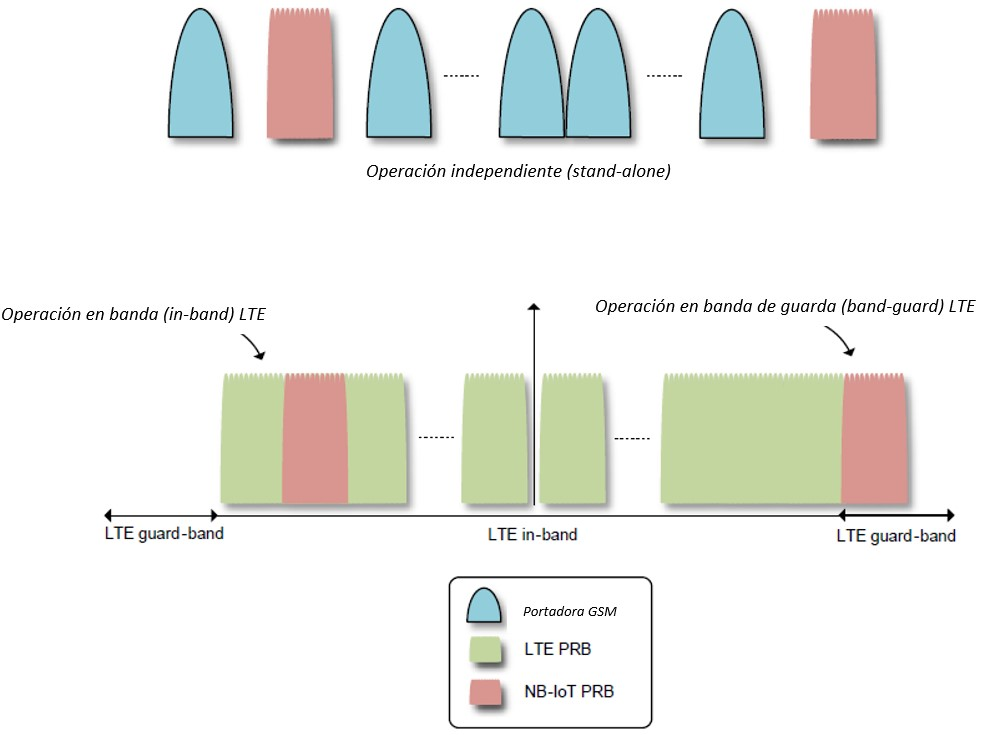
\includegraphics[scale=.7]{modooperacionNBIOT}
    \decoRule
    \caption[Modos de Operación en NB-IoT.]{Modos de Operación en NB-IoT. \parencite{Liberg2018}}
    \label{fig:NBIoT}
\end{figure}
    
En esta especificación también se detallan algunos aspectos de tráfico en términos de los tamaños de paquetes que se esperan para NB-IoT. Se definen cuatro tipos de aplicaciones de tráfico diferentes.

\subsubsection{Reportes autónomos móviles (MAR, \textit{Mobile Autonomous Reporting}}
\subsubsection{Informes de excepción}
Se espera que muchas aplicaciones de tipo sensor monitoreen una condición física y activen un informe de excepción cuando se detecte un evento. Estos eventos serán, en general, raros y ocurrirán cada pocos días, meses o incluso años. Ejemplos de tales aplicaciones incluyen detectores de alarma de humo, notificaciones de fallas de energía de medidores inteligentes, notificaciones de manipulación, etc.\newline

Para el análisis de latencia, se supone que los informes de excepción MAR tienen una carga útil de la aplicación de enlace ascendente de 20 bytes. Se requiere que dichos informes se entreguen casi en tiempo real, con un objetivo de latencia de 10 segundos.\newline

Para cada informe de enlace ascendente generado (es decir, el 100\% de los informes de excepción de enlace ascendente), también se supone que la aplicación enviará un ACK de aplicación de enlace descendente. El tamaño del tamaño ACK de la capa de aplicación es cero. El tamaño total del paquete (por encima del equivalente de la capa SNDCP) es la sobrecarga debida COAP / DTLS / UDP / IP.\newline

\subsubsection{Informes periódicos}

Se espera que los informes periódicos de enlace ascendente sean comunes para aplicaciones de IoT celular como informes de medición de servicios inteligentes (gas / agua / electricidad), agricultura inteligente, entorno inteligente, etc. El modelo de tráfico de informes de enlace ascendente periódico MAR se utiliza en simulaciones a nivel de sistema para análisis de capacidad.\newline

Distribución del tamaño de la carga útil de la aplicación. UL. Sigue una distribución de Pareto con parámetro alfa = 2.5 y tamaño mínimo de carga útil de la aplicación = 20 bytes con un corte de 200 bytes, es decir, las cargas superiores a 200 bytes serán limitadas a 200 bytes.\newline

Se supone un ACK de capa de aplicación DL para un evento de informe periódico de enlace ascendente en el 50\% de los informes periódicos UL MAR generados. Se supone que el tamaño de la carga útil ACK del enlace descendente de la aplicación es de 0 bytes. El tamaño total del paquete (superior al equivalente de la capa SNDCP) es la sobrecarga debida a COAP / DTLS / UDP / IP y se envía inmediatamente después de que la estación base recibe con éxito un paquete UL de aplicación.\newline

Entonces, una vez revisadas estas clasificaciones de tráfico compatibles para NB-IoT, se procede a agrupar estos tipos de tráfico con los escenarios que se consideraron en la \textit{Tabla 8} de la sección anterior, de tal manera que se establezcan las condiciones base de un ambiente NB-IoT de acuerdo a los servicios seleccionados (secXXXX).\newline

La adición de la columna ``Tamaños de paquete'' para la \textit{Tabla~\ref{tab:}} se da en la \textit{Tabla~\ref{tab:}}\newline

\begin{table}
\caption{Caracterización del tráfico de paquetes en aplicaciones seleccionadas para la simulación.}
\label{tab:trafpkt}
\centering
\begin{tabular}{*{2}{m{7cm}}}\\ 
\textbf{\textit{Servicio}} & \textbf{Tamaño de paquetes} \\ 
\textit{Control de iluminación (Smart City) } & \footnotesize{ Activación aleatoria \textbf{UL}: 20 bytes \textit{payload} \textbf{DL}: ACK de 0 bytes } \\ \hline 
\textit{Monitoreo del consumo de agua y electricidad en la ciudad (Smart City) } & \footnotesize{ Activación periódica \textbf{UL}: distribución de Pareto con parámetro alfa = 2.5 y tamaño mínimo de carga útil de la aplicación = 20 bytes con un corte a 200 bytes \textbf{DL}: ACK de 0 bytes 50\% de las veces. } \\ \hline 
\textit{Detección de terremotos (Smart Environment)}  & \footnotesize{ Activación aleatoria \textbf{UL}: 20 bytes \textit{payload} \textbf{DL}: ACK de 0 bytes } \\ \hline 
\textit{Monitoreo de contaminación del aire (Smart Environment) } & \footnotesize{ Activación periódica \textbf{UL}: distribución de Pareto con parámetro alfa = 2.5 y tamaño mínimo de carga útil de la aplicación = 20 bytes con un corte a 200 bytes \textbf{DL}: ACK de 0 bytes 50\% de las veces. } \\ \hline 
\textit{Control dinámico de semáforos (Smart Transport and Mobility)}  & \footnotesize{ Activación aleatoria \textbf{UL}: distribución de Pareto con parámetro alfa = 2.5 y tamaño mínimo de carga útil de la aplicación = 20 bytes con un corte a 200 bytes \textbf{DL}: ACK de 0 bytes 50\% de las veces. } \\ \hline 
\textit{Genérico}  & \footnotesize{ Activación aleatoria \textbf{UL}: 20 bytes \textit{payload} \textbf{DL}: ACK de 0 bytes } \\  
\end{tabular}
\end{table}


%----------------------------------------------------------------------------------------
%	SECTION 
%----------------------------------------------------------------------------------------

\section{INDICADORES CLAVE DE RENDIMIENTO (KPIs)}

Hay muchas formas de medir el rendimiento de una red, por medio de sus características se pueden definir los indicadores clave de rendimiento para la evaluación integral, precisa y eficiente de las tecnologías de red 5G.\newline

Con la profundización de la investigación de la tecnología 5G, se puede prever que habrá nuevos indicadores de evaluación. El diseño de estos indicadores directamente medibles, por un lado, necesita combinar las características de los nuevos servicios, y por otro lado, debe aprender completamente de la experiencia de los KPI clásicos de generaciones anteriores como lo son: el \textit{throughput, }dada una\textit{ }probabilidad de salida y la latencia. La densidad de conexión, la densidad de volumen de tráfico y el consumo de energía son nuevos KPI introducidos por las redes 5G/IoT \parencite{WirelessSim}.\newline

Para cumplir con el conjunto de requisitos de mMTC, NB-IoT debe admitir principalmente cuatro indicadores clave de rendimiento (KPI).\newline

\begin{enumerate}
\item  Vida útil de la batería del dispositivo más allá de 10 años, suponiendo una capacidad de energía almacenada de 5 Wh.
\item  Densidad de conexión masiva de hasta 1M dispositivos por km cuadrado en un entorno urbano.
\item  Latencia de como máximo 10 s.
\item  Una tasa máxima alcanzable de hasta 200kbps (subida).
\end{enumerate}

El análisis fundamental del simulador contemplará como métricas de desempeño a la compensación entre la tasa máxima alcanzable y la densidad de usuarios atendidos en términos de una calidad de servicio QoS. Esta QoS dependerá de los cuatro principales KPIs para mIoT.\newline

Por lo tanto, de acuerdo a las métricas que serán consideradas, los KPIs a considerar son: la tasa máxima alcanzable y la densidad de usuarios, sin embargo durante las investigaciones que hemos realizado en la literatura científica no hemos encontrado ningún artículo que proponga un modelo de sistema que alcance el KPI de soportar hasta 1 millón de dispositivos. Por lo que para esta métrica se buscará un diseño de sistema tal que a un determinado tope de usuarios se logre una óptima tasa UL, es decir, el dimensionamiento de la red.

%----------------------------------------------------------------------------------------
%	SECTION 
%----------------------------------------------------------------------------------------

\section{ANÁLISIS DE MODELOS PARA LA EVALUACIÓN DE REDES 5G/IoT}
En el modelado de redes 5g / IoT entran diferentes aspectos para representar y caracterizar el comportamiento correcto de estas redes. Para este caso, desde el punto de vista de simulaciones a nivel de sistema, los modelos se suelen concentrar en las capas superiores de la pila TCP / IP.\newline

Los aspectos más importantes y considerados en la literatura \parencite{WirelessSim}, son:

\begin{enumerate}
    \item  Modelo de despliegue de BSs y UEs.
    \item  Modelo de antenas (MIMO, MISO, entre otras) y formación de haz.
    \item  Modulación y codificación.
    \item  Modelo de canal.
    \item  Patrones de Movilidad.
    \item  Calendarizadores (planificadores de recursos).
    \item  Esquema de acceso múltiple al medio.
    \item  Modelos de tráfico.
\end{enumerate}

Como se puede leer, una simulación se puede realizar tan compleja como se desee, para este proyecto se contemplan solamente algunos de estos aspectos que son compatibles para una simulación a nivel de sistema. Estas simulaciones dan una buena estimación de un análisis fundamental desde la perspectiva del dimensionamiento que puede alcanzar una red.\newline
Los modelos que se incluyen en el simulador son los siguientes:

\subsection{MODELO DE DESPLIEGUE DE BSs Y UEs}

La teoría del diseño celular da una forma simplificada de un diseño idealizado para redes móviles, esta se desarrolló en la literatura desde el comienzo del concepto celular [1975 aprox.], sin embargo este despliegue uniforme que propone la teoría celular, es poco realista ya que nunca se tiene una instalación regular, esto debido a que la densidad del tráfico varia espacial y temporalmente. En el despliegue de BS, frecuentemente en ubicaciones donde se concentraba mayor cantidad de tráfico lo que se realiza es instalar otra BS y por lo tanto esto rompe con esta uniformidad.\newline

En el modelado de posicionamiento de las estaciones base y los nodos IoT existen diferentes estrategias de despliegue (como se puede ver en la \textit{Figura~\ref{fig:BSs}}) y es de mucha importancia dependiendo los objetivos de la simulación, es decir, para un alcance comercial resulta importante simular el despliegue determinístico de los actores de la red de acuerdo al escenario donde se vaya a montar una determinada red, por otro lado para un alcance con fines de análisis en el diseño y dimensionamiento de estas redes resulta más adecuado un despliegue aleatorio. \newline

\begin{figure}[th]
\centering
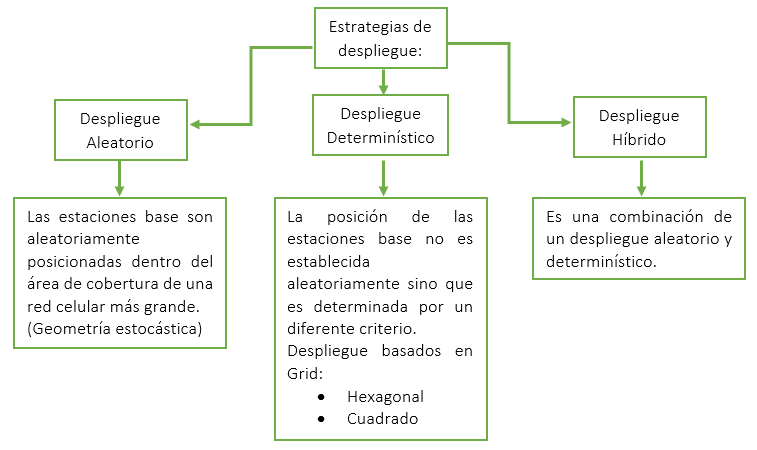
\includegraphics[scale=1]{Diferentes estrategias de despliegue para BSs}
\decoRule
\caption[Diferentes estrategias de despliegue para BSs]{Diferentes estrategias de despliegue para BSs}
\label{fig:BSs}
\end{figure}

Muchos autores coinciden en que varias distribuciones de redes móviles siguen un proceso estocástico \parencite{Kouzayha2018}\parencite{Zhang2017}. La geometría estocástica es una rama de la probabilidad con muchas aplicaciones que permiten el estudio de fenómenos aleatorios en el plano o en dimensiones superiores \parencite{Haenggi2009}. Está intrínsecamente relacionada con la teoría de los procesos puntuales. Inicialmente su desarrollo fue estimulado por aplicaciones en biología, astronomía y ciencias de los materiales. Hoy en día, también se utiliza en análisis de imágenes y en el contexto de redes de comunicación. Recientemente se ha utilizado con éxito para modelar la distribución espacial de células pequeñas como las femtoceldas \parencite{TurjmanSmallCells}. \newline

Para esto, la distribución de terminales móviles se realiza de acuerdo con varios procesos de punto estacionario de Poisson independientes con intensidad \textit{$\lambda$m}. Con un PPP estacionario, la distancia entre un terminal móvil y su BS de servicio se distribuye independientemente de la ubicación exacta del terminal móvil.\newline

En este proyecto no se propone simular un ambiente uniforme, establecido o determinístico por lo que se seguirá el despliegue de una geometría estocástica siguiendo un PPP.\newline

% \parencite{}
\myworries{colocar PPP}
\subsubsection{Poisson Point Process}


\subsection{MODELO DE CANAL}

Para conducir al diseño preciso y confiable de un sistema 5G es necesario tener buen conocimiento de las características del canal de propagación a través de las frecuencias de microondas y ondas milimétricas. \newline

Los modelos de canal son necesarios para simular la propagación de una manera reproducible y rentable, y se utilizan para diseñar y comparar con precisión las interfaces de radio aire y el despliegue del sistema. Los parámetros comunes del modelo de canal inalámbrico incluyen frecuencia de portadora, ancho de banda, distancia 2D o 3D entre el transmisor (Tx) y el receptor (Rx), los efectos ambientales y otros requisitos necesarios para construir equipos y sistemas estandarizados a nivel mundial. El desafío definitivo para un modelo de canal 5G es proporcionar una base física fundamental, a la vez flexible y precisa, especialmente en un amplio rango de frecuencias como 0.5--100 GHz \parencite{Rappaport2017}. Los modelos de canal investigados se dividen principalmente de acuerdo al escenario en el que se están diseñando, ya sea \textit{Urban Macro (UMa) o Urban Micro (UMi)}, además de la condición del ambiente si es que hay línea de vista (\textit{LoS}) entre el UE y la BS.\newline

Existe una gama amplia de modelos de canal propuestos para redes 5G, (p.ej. 3GPP, WINNER I/II, QuaDRiga/ mmMagic, 5GCM, METIS, MiWEBA, IEEE \parencite{WirelessSim}). Aunque existen diversos modelos, los modelos de canal 3GPP y WINNER II son los más conocidos y empleados en la industria de comunicaciones móviles \parencite{Sun2016}, conteniendo una gran diversidad de escenarios de despliegue como lo son \textit{UMi, UMa, indoor office (InH)}, etc. Además proveen parámetros clave del canal incluyendo probabilidades de línea de vista (\textit{LoS}), modelos de pérdida por trayectoria, retardos y niveles de potencia por trayectoria \parencite{Sun2016}. \newline

En la búsqueda del modelo de canal a implementar en el simulador nos enfocamos en buscar un modelo teórico y estocástico en vez de uno empírico, ya que nuestro proyecto va más enfocado en el teletráfico. Los modelos empíricos suelen ser más sofisticados y piden una gran cantidad de parámetros de entrada. Por lo tanto buscamos los modelos estocásticos que se adaptaran al rango de frecuencia de transmisión y a los ambientes urbanos que se proponen.\newline

En \parencite{Sun2016}, los autores evaluaron tres diferentes modelos de propagación estocásticos de perdida por trayectoria a larga escala para ser implementados a través de la banda de frecuencias de microondas y ondas milimétricas. ABG, CI y CIF son modelos estadísticos de propagación para multi-frecuencias (estocásticos) que describen los parámetros de larga escala con pérdida de trayectoria de acuerdo a la distancia.

Los modelos evaluados fueron: 
\begin{enumerate}
\item  ABG: Modelo Alpha-Beta-Gamma.
\item  CI: Modelo de pérdida por trayectoria de distancia de referencia de espacio libre cercano.
\item  CIF: Modelo CI con un exponente de pérdida de trayectoria ponderado en frecuencia.
\end{enumerate}

 Para el primero, la ecuación del modelo ABG está dada por:
 \begin{equation}
    L^{ABG}_p(f,d)_{\left[dB\right]}=10alpha {\ log}_{10}\left(\frac{d}{1m}\right)+\beta +\ 10gamma {\ log}_{10}\left(\frac{f}{1GHz}\right)+\ x^{ABG}_{\sigma .}, donde\ d\ge 1m
    \label{eqn:ABG}
\end{equation}

\[\alpha \to coeficiente\ que\ representa\ la\ dependencia\ de\ la\ perdida\ por\ trayectoria\ con\ la\ distancia\] 
\[\gamma \to coeficiente\ que\ representa\ la\ dependencia\ de\ la\ perdida\ por\ trayectoria\ con\ la\ frecuencia\] 
\[\beta \to es\ un\ valor\ de\ compensación\ para\ la\ pérdida\ por\ trayectoria\ (en\ dB's)\] 
\[x^{ABG}_{\sigma .}\to es\ una\ variable\ aleatoria\ gaussiana\ de\ media\ cero\ con\ una\ desviaci\textrm{ó}n\ est\textrm{á}ndar \]
\[sigma \ [dB], que\ describe\ las\ fluctuaciones\ de\ se\textrm{ñ}al\ a\ gran\ escala\ (es\ decir,\ multitrayectoria)\]
\[desvanecimiento\ tipo\ Rayleigh \] 

Para el segundo, la ecuación del modelo CI está dada por:
\begin{equation}
    L^{CI}_p(f,d)_{\left[dB\right]}=32.4+\ 10\ n{\ log}_{10}\left(\frac{d}{d_0}\right)+{\ 20\ log}_{10}\left(d_0\right)+{20\ log}_{10}\left(f\right)+x^{CI}_{\sigma .}, donde\ d\ge d_0
    \label{eqn:CI}
\end{equation}
\[x^{CI}_{\sigma .}\to es\ una\ variable\ aleatoria\ gaussiana\ de\ media\ cero\ con\ una\ desviaci\textrm{ó}n\ est\textrm{á}ndar \]
\[sigma \ [dB], que\ describe\ las\ fluctuaciones\ de\ se\textrm{ñ}al\ a\ gran\ escala\ (es\ decir,\ multitrayectoria)\]
\[desvanecimiento\ tipo\ Rayleigh\] 

Para el tercero, la ecuación del modelo CIF está dada por:
\begin{equation}
    L^{CIF}_p(f,d)_{\left[dB\right]}=32.4+\ 10\ n{\left(1+b \left(\frac{f-f_0}{f_0}\right) \right)log}_{10}\left(d\right)+{20\ log}_{10}\left(f\right)+x^{CIF}_{\sigma .},  donde\ d\ge 1m
    \label{eqn:CIF}
\end{equation}
\[x^{CIF}_{\sigma .}\to es\ una\ variable\ aleatoria\ gaussiana\ de\ media\ cero\ con\ una\ desviaci\textrm{ó}n\ est\textrm{á}ndar  \]
\[ sigma \ [dB], que\ describe\ las\ fluctuaciones\ de\ se\textrm{ñ}al\ a\ gran\ escala\ (es\ decir,\ multitrayectoria)\]
\[desvanecimiento\ tipo\ Rayleigh\] 

Cada uno de estos modelos han sido recientemente estudiados por organizaciones de estandarización como 3GPP y son propuestos para el uso en el diseño de sistemas inalámbricos de comunicación de 5G enfocados en escenarios \textit{UMa, UMi, InH,y SM}.\newline

De acuerdo al análisis de sensibilidad en \parencite{Sun2016}, se demostró que el modelo CI es el más adecuado para entornos al aire libre debido a su precisión, simplicidad y rendimiento de sensibilidad, dado que la pérdida de trayectoria medida depende poco de la frecuencia en ambientes exteriores más allá del primer metro de propagación de espacio libre.\newline

Por otro lado, el modelo CIF es muy adecuado para entornos interiores, ya que proporciona una desviación estándar más pequeña que el modelo ABG en muchos casos, incluso con menos parámetros del modelo y tiene una precisión superior cuando se analiza con el análisis de sensibilidad.\newline

Los modelos CI y CIF son más robustos y precisos en comparación con el modelo ABG, por lo que es confiable la aplicación del modelo CI para simular entornos en exteriores y el CIF para interiores \parencite{Sun2016}.\newline

De acuerdo a lo propuesto en la \textit{sección \ref{} }, el ambiente urbano que consideraremos está dirigido a un entorno en exteriores por la aplicación de los sensores a implementar. Por lo que se selecciona al modelo CI (Modelo de pérdida por trayectoria de distancia de referencia de espacio libre cercano) como el que ayudará a caracterizar las perdidas por trayectoria y desvanecimiento por el canal. 

Los parámetros que solicita este modelo (\textit{Ecuación~\ref{eqn:CI}}) son: la distancia en 3D entre la BS y el UE, la frecuencia fundamental de operación y una variable aleatoria de media cero con una desviación estándar $\sigma$ [dB], que describirá las fluctuaciones de señal a gran escala (es decir, la multitrayectoria[\textit{multipath}]) . Además de esto también pide un valor d${}_{0}$ que es la distancia cercana de referencia al espacio libre, los autores proponen a d${}_{0}$ = 1 m en modelos de pérdida de trayectoria 5G ya que las distancias de cobertura serán más cortas a frecuencias más altas. 


\subsection{ESQUEMA DE ACCESO MÚLTIPLE AL MEDIO}

\subsubsection{Acceso Múltiple No Ortogonal (NOMA)}

El acceso múltiple no ortogonal (NOMA) se ha convertido en un principio importante para el diseño de técnicas de acceso por radio para las redes inalámbricas de quinta generación (5G) \parencite{DIng2017}. NOMA se puede clasificar en dos categorías, el dominio de código NOMA (CD-NOMA) y el dominio de potencia NOMA (PD-NOMA). CD-NOMA utiliza diferentes códigos en el mismo recurso para lograr una ganancia de multiplexación, mientras que PD-NOMA asigna a los usuarios niveles de potencia distintos para maximizar el rendimiento. En comparación con el acceso múltiple ortogonal (OMA) que se ha aplicado ampliamente en los sistemas de comunicación inalámbrica existentes, NOMA posee el potencial de mejorar aún más la eficiencia espectral del sistema y la capacidad de conectividad.\newline

Como se mencionaba, PD-NOMA utiliza el dominio de la potencia para el acceso múltiple donde diferentes usuarios son servidos con diferentes niveles de potencia, como las señales de los diferentes usuarios se sobreponen, los receptores aprovechan la cancelación sucesiva de interferencia (SIC) para distinguir a cada una. Como varios usuarios son admitidos en la misma ranura de tiempo, frecuencia o código, la interferencia co-canal será fuerte en los sistemas NOMA \parencite{Ding2016}, por lo que no es realista el asegurar a todos los usuarios del sistema que utilicen NOMA conjuntamente, por esta razón, una alternativa es utilizar un esquema hibrido donde NOMA sea combinado con el esquema convencional ortogonal OMA. El rendimiento de este esquema hibrido es muy dependiente de como los usuarios son agrupados \parencite{Ding2016}. El agrupamiento de usuarios seleccionara a los usuarios con los que se les asignará el mismo bloque de recursos ortogonales.\newline

\begin{figure}[th]
\centering
\includegraphics[scale=1]{Figures/Cancelación Sucesiva de Interferencia (SIC)}
\decoRule
\caption[Cancelación Sucesiva de Interferencia (SIC)]{Cancelación Sucesiva de Interferencia (SIC), [Fuente: R. Kizilirmak 2017]}
\label{fig:SIC}
\end{figure}

En la \textit{Figura~\ref{fig:SIC}}, las dos señales de información indicadas con diferentes colores se superponen en el transmisor. La señal recibida en el receptor SIC incluye todas estas tres señales. La primera señal que SIC decodifica es la más fuerte, mientras que la otra es tratada como ruido. La primera señal decodificada se resta de la señal recibida y si la decodificación es perfecta, la forma de onda con la otra señal se obtiene con precisión. SIC itera el proceso hasta que encuentra la señal deseada \parencite{Kizilirmak2016}.\newline

\begin{figure}[th]
\centering
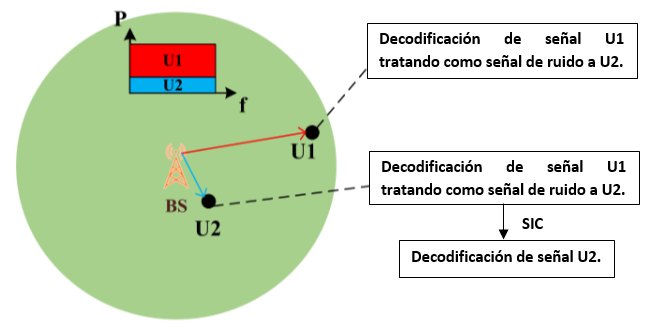
\includegraphics[scale=1]{Figures/Ejemplo del esquema NOMA en un enlace de bajada con dos usuarios y una sub-portadora}
\decoRule
\caption[Ejemplo del esquema NOMA en un enlace de bajada con dos usuarios y una sub-portadora.]{Ejemplo del esquema NOMA en un enlace de bajada con dos usuarios y una sub-portadora, [Fuente: Ding 2017]}
\label{fig:NOMADL}
\end{figure}

Como se muestra en la \textit{Figura~\ref{fig:NOMADL}}, la idea clave del NOMA en el dominio de potencia es asignar más potencia al usuario con condiciones de canal más pobres. El usuario 1 decodifica su propio mensaje directamente tratando el mensaje del usuario 2 como ruido y por otro lado, el usuario 2 realiza SIC, es decir, primero decodifica el mensaje del usuario 1 y luego elimina este mensaje de su observación antes de decodificar su propio mensaje.

Suponga que el usuario 1 es un dispositivo IoT que requiere solo una baja velocidad de datos, y el usuario 2 es un usuario que exige una alta velocidad de datos. Cuando se utiliza OFDMA, que es un ejemplo típico de OMA, cada usuario se asigna a la sub-portadora. En este ejemplo, la eficiencia espectral de OMA es pobre ya que el dispositivo IoT tiene más ancho de banda de lo que realmente necesita, mientras que al usuario de banda ancha no se le asigna suficiente ancho de banda. Por otro lado, el uso de NOMA fomenta el intercambio de espectro, es decir, el usuario de banda ancha también puede tener acceso a la sub-portadora ocupada por el dispositivo IoT, en la F\textit{igura 24} se puede observar gráficamente la asignación del espectro en los dos esquemas.

\begin{figure}[th]
\centering
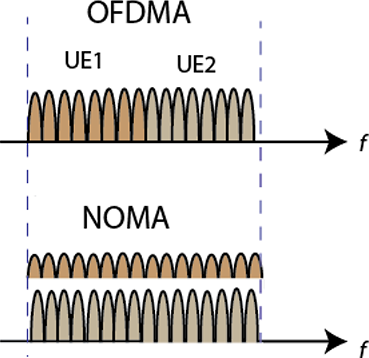
\includegraphics[scale=1]{Figures/Ejemplo del espectro compartido para OFDMA y NOMA con dos usuarios}
\decoRule
\caption[Ejemplo del espectro compartido para OFDMA y NOMA con dos usuarios.]{Ejemplo del espectro compartido para OFDMA y NOMA con dos usuarios, [Fuente: R. Kizilirmak 2017]}
\label{fig:OFDMANOMA}
\end{figure}

Dada la madurez técnica de OFDMA, es muy probable que este tipo de OMA se incorpore a las redes 5G \parencite{DIng2017} y la forma en que múltiples sub-portadoras OFDMA se pueden combinar de manera eficiente con NOMA ha recibido mucha atención.

Acerca del uso de arreglos múltiples de antenas, estos aún no han sido estudiados para poder alcanzar un rendimiento óptimo del sistema, el ordenamiento de usuarios en escenarios de MIMO-NOMA es una tarea difícil \parencite{DIng2017}. En el caso de SISO, los canales de los usuarios son escalados, por lo que es sencillo ordenar a los usuarios de acuerdo con las condiciones de su canal. Sin embargo, cuando los nodos están equipados con antenas múltiples, los canales de los usuarios están en forma de vectores o matrices, lo que significa que ordenar a los usuarios de acuerdo con las condiciones de sus canales como en el caso SISO se vuelve difícil. 

Como resultado, el uso de NOMA soporta eficientemente la conectividad masiva y cumple con los diversos requisitos de QoS de los usuarios. El diseño de NOMA en transmisiones de subida (\textit{uplink}) ha sido propuesto en \parencite{Al-Imari2014} y el diseño óptimo de NOMA en transmisiones de bajada (\textit{downlink}) ha sido propuesto en \parencite{Zhu2019}.

Por una parte, en \parencite{Zhang2017} se implementó NOMA emparejando selectivamente dos usuarios, es decir, se escogía a un usuario con una condición de canal muy buena (cerca de la BS) y otro con una condición de canal muy pobre (en el borde de la celda). Por otro lado en \parencite{Shahini2019}, se implementó NOMA usando la técnica de agrupamiento de usuarios, para esto, considerando un entorno donde conviven dispositivos mMTC y URLLC (mayores requisitos de velocidad de datos en comparación con los dispositivos mMTC), de igual manera se agrupan a un grupo de usuarios (p.ej., 2, 3 o 4 usuarios) de diferente tipo (mMTC y URLLC), se ordenan convenientemente para implementar SIC.

Entonces, como vemos hay dos maneras de implementar NOMA. Las dos son propuestas que han sido estudiadas para para cubrir los requerimientos de mMTC ya que NB-IoT no es capaz de proveer conectividad a una cantidad masiva de dispositivos IoT como se espera en el futuro.

Por lo tanto, en el simulador se propone implementar NOMA usando la técnica de agrupamiento de usuarios, en nuestro caso como consideraremos dos tipos de clase de sensores NB-IoT clase I y clase II (con mayores requisitos de velocidad de datos en comparación con clase I). La relación de la distribución de dispositivos clase 1 con los de clase 2 será de 3 a 1. Con el fin de que por lo menos se un dispositivo de clase II se agrupe con tres de clase I.

\subsection{MODELOS DE TRÁFICO}

Los modelos de tráfico en comunicaciones móviles buscan acercarse, lo más posible a cómo transmiten datos o realizan peticiones de acceso los dispositivos que intentan modelar. Estos modelos de tráfico pueden clasificarse en modelos de tráfico\textbf{ }agregado y modelos de tráfico fuente \parencite{Laner2013}, el tráfico agregado simula un flujo de tráfico que se agrupa para recibir un tratamiento común, mientras que en los modelos de tráfico fuente es justamente cada una de las fuentes generadoras del tráfico la que se simula y frecuentemente se hace acompañada de una cadena de Markov que intenta representar los distintos estados del dispositivo fuente y la probabilidad de transición entre ellos.\newline

Sin importar el modelo de tráfico a utilizar, en \parencite{Laner2013} se señala que los modelos de tráfico que pretendan simular el comportamiento de dispositivos de MTC (\textit{Machine Type Communications}) deben:

\begin{itemize}
\item  Capturar con precisión el comportamiento de un solo dispositivo de MTC 
\item  Permitir la simulación concurrente de una cantidad masiva de dispositivos con su potencial reacción síncrona a un evento.
\end{itemize}

La importancia de la elección correcta de un modelo de tráfico para los dispositivos IoT recae en un diseño correcto y la optimización futura de la red y el cumplimiento de su respectiva QoS sin comprometer los servicios convencionales de datos, voz y video. Sin embargo, antes de elegir un modelo es importante conocer las propiedades del tráfico máquina a máquina (M2M, \textit{Machine to Machine}), el cual se considera una forma de transmisión de datos que no requiere necesariamente de la interacción humana (ETSI, 2010) y corresponde justamente al tráfico de los nodos IoT, de \parencite{Laner2013} tenemos:

\begin{itemize}
\item  Cantidad masiva de dispositivos
\item  Pocos paquetes de un tamaño pequeño a ser transmitidos por dispositivo
\item  Periodos largos entre dos transmisiones consecutivas
\item  Tráfico de subida (\textit{uplink)} dominante
\item  Transmisiones en tiempo real y transmisiones tolerantes al retraso
\item  Paquetes no sincronizados y paquetes sincronizados
\item  Activación de tráfico que depende del espacio y tiempo
\end{itemize}

Además, se hace  la distinción de 3 patrones de tráfico que pueden presentarse en estos dispositivos:

\begin{enumerate}
    \item \underbar{Actualización periódica (PU, }\textit{\underbar{Periodic Update}}\underbar{):} Este tipo de tráfico ocurre cuando el dispositivo transmite reportes de estado y/o actualizaciones de estado de manera periódica. Puede verse como una activación por evento que ocurre por el mismo dispositivo en un intervalo periódico. Típicamente, el tráfico PU no necesita transmitirse en tiempo real y cuenta además de un patrón periódico de tiempo con un tamaño constante en sus paquetes. Un ejemplo típico de estos dispositivos son medidores inteligentes (por ejemplo gas, electricidad, agua).
    \item \underbar{Activación por evento (ED, }\textit{\underbar{Event-Driven}}\underbar{):} En caso de que un evento desencadene la transmisión de datos de un dispositivo, el patrón de tráfico corresponde a esta segunda clase. Un evento puede ser causado ya sea por la medición de un parámetro que sobrepasó un límite y activó alguna alarma o bien por el nodo que actúa como servidor y envía comandos al dispositivo. El tráfico \textit{Event-Driven} puede requerir ser transmitido tanto en tiempo real o no, un ejemplo de mensajes de subida que debieran ser transmitidos en tiempo real son alarmas y notificaciones médicas de emergencia, en cuanto a los mensajes de bajada, estos podrían ser la distribución de mensajes de emergencia locales, por ejemplo en caso de sismo o tsunamis. En algunos casos, como ya se mencionó, este tráfico no necesita ser transmitido en tiempo real. Por ejemplo, cuando un dispositivo IoT envía una actualización de su ubicación al servidor o se reciba una actualización de \textit{firmware }desde este.
    \item \underbar{Intercambio de carga útil (PE, }\textit{\underbar{Payload Exchange}}\underbar{):} este último tipo de tráfico ocurre después de una transmisión previa (PU o ED). Comprende todos los casos en los que es necesario un mayor intercambio de datos entre el dispositivo que envía y su servidor, este tráfico se espera sea predominantemente de subida y puede ser de tamaño constante o variable según la aplicación.\newline
\end{enumerate}

Las aplicaciones en el mundo real que implementan dispositivos de IoT serán casi siempre una combinación de estos tipos de tráfico más un estado de reposo o de ahorro de batería.\newline

\begin{figure}[th]
\centering
\includegraphics[scale=1]{Figures/Estructura de los estados principales del tráfico M2M}
\decoRule
\caption[Estructura de los estados principales del tráfico M2M]{Estructura de los estados principales del tráfico M2M}
\label{fig:}
\end{figure}

Ahora se presentan los modelos de tráfico más recurrentes en la literatura para la simulación de comunicaciones M2M.\newline

\subsubsection{Modelos de tráfico agregado}

Han sido propuestos por la 3GPP al reconocer la importancia de caracterizar el tráfico M2M. Se trata en realidad de 2 modelos de tráfico agregado generado por una gran cantidad de usuarios, el primero modela el tráfico generado de forma aleatoria y el segundo modela tráfico síncrono en el tiempo, esto se puede observar en la \textit{Tabla~\ref{tab:trafico3gpp}}.\newline

\begin{itemize}
\item  \textit{Modelo 1} - Modelo de tráfico agregado sin correlación 3GPP: Genera tráfico sin correlación en un intervalo específico de tiempo. Lo que significa que no se tomarían en cuenta la correlación entre los dispositivos IoT. Utiliza una distribución uniforme para modelar el tráfico agregado en un intervalo de tiempo específico.
\item  \textit{Modelo 2 -} Modelo de tráfico agregado con correlación 3GPP: Este modelo genera tráfico correlacionado en un intervalo de tiempo, asumiendo que todas las máquinas se encuentran sincronizadas. Utiliza una distribución beta para modelar en tráfico agregado en un intervalo de tiempo específico.
\end{itemize}

\begin{table}
\caption{Modelos de tráfico agregado propuestos por la 3GPP para comunicaciones M2M}
\label{tab:trafico3gpp}
\centering
\begin{tabular}{*{2}{m{8.5cm}}}\\
\textbf{Sincronizado/Coordinado/Correlacionado\newline (En un intervalo limitado en el tiempo)} & \textbf{No sincronizado/No coordinado/ No correlacionado\newline (En un intervalo limitado en el tiempo)} \\ \hline
Distribución de probabilidad de arribo de paquetes/peticiones f(t) en [0,1] : \underbar{Beta} (3,4) & Distribución de probabilidad de arribo de paquetes/peticiones f(t) en [0,1]: \underbar{Uniforme} \\ 
Número de dispositivos: 1 000, 3 000, 5 000, 10 000, 30 000. & Número de dispositivos: 1 000, 3 000, 5 000, 10 000, 30 000. \\ 
Periodo \textit{T }: 10 s & Periodo \textit{T }: 60 s \\ 
\end{tabular}
\end{table}

La principal ventaja de los modelos de tráfico agregado es su fácil implementación (en términos de una baja complejidad computacional) cuando se simulan una gran cantidad de dispositivos. Por otro lado, como se menciona en \parencite{IoTTrafficHossfeld}, la precisión de estos modelos al reflejar el comportamiento real del sistema es su principal desventaja.

\subsubsection{Modelos de tráfico fuente}

Los modelos de tráfico fuente de dispositivos MTC, modelan justamente el tráfico que genera cada uno de los dispositivos. Este tipo de modelado es más preciso que el de tráfico agregado ya que modela el comportamiento de cada fuente, sin embargo, puede fácilmente volverse muy complejo cuando se agrega una gran cantidad de dispositivos (fuentes). A continuación se presentan y analizan dos modelos de tráfico fuente.\newline

\begin{itemize}
\item  \textit{Modelo 3:} Modelo de fuente de \textit{Semi-Markov} (\textit{Semi-Markov Models, SMM)}\\

En este modelo de fuente cada dispositivo se modela utilizando una cadena de Markov en la que se define la probabilidad de transición entre estados. Los estados que se encontrarán casi siempre modelados son los mencionados anteriormente: el de actualización periódica (PU), el de activación por evento (ED) y el de intercambio de carga útil. La \textit{Figura~\ref{fig:SMM}} muestra cómo se verían modelados los estados de un dispositivo en una cadena de Markov.\newline

La probabilidad de transición entre el mismo estado es 0, además los tiempos de espera y la longitud de los mensajes son generados de acuerdo a una distribución de probabilidad que es independiente de cada estado y potencialmente distinta para cada uno de ellos \parencite{IoTTrafficHossfeld}.\newline

\begin{figure}[th]
\centering
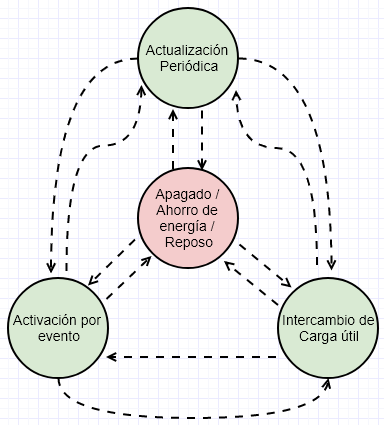
\includegraphics[scale=1]{Figures/Cadena de Markov del modelo SMM}
\decoRule
\caption[Cadena de Markov del modelo SMM]{Cadena de Markov del modelo SMM}
\label{fig:SMM}
\end{figure}

La principal ventaja del modelo de tráfico fuente SMM es que permitiría una descripción más detallada del comportamiento de los dispositivos IoT de manera individual, sin embargo no es capaz de capturar la relación que existe entre dos dispositivos cercanos que pudieran tener una cierta sincronía entre ellos, otra desventaja es que la complejidad del sistema aumenta considerablemente entre más dispositivos se simulan a diferencia de los modelos de tráfico agregado.\newline

\item  \textit{Modelo 4:} Modelo de fuente de Procesos de Poisson emparejados Markov-modulados (CMMPP\textit{, Coupled Markov Modulated Poisson Process)}

En el modelo de tráfico CMPP cada dispositivo MTC es representado como una entidad por separado en el que a diferencia del modelo SMM sí puede representarse una sincronización espacial y temporal entre dispositivos similares. La clave en el diseño del modelo CMMPP se presenta en encontrar un balance entre el emparejamiento entre distintos dispositivos y una complejidad tolerable del sistema cuando se tiene una gran cantidad de dispositivos \parencite{Gupta2018}.

Los procesos de Poisson Modulados con Markov (\textit{Markov modulated Poisson processes, MMPP}) consisten en procesos de Poisson que son modulados por la tasa $\lambda_{i[t]}$, que viene determinada por el estado de una cadena de Markov $sn[t]$, este principio se ve presentado en la \textit{Figura~\ref{fig:CMMPP}} donde \textit{p${}_{i,j}$}${}_{\ }$son las probabilidades de transición entre los estados de la cadena. En este modelo cada dispositivo \textit{n} del total\textit{ N} se encuentra representado por una cadena de Markov y un correspondiente proceso de Poisson. Debido a que existe una alta correlación en el cambio de estados de distintos dispositivos, tanto en el espacio como en el tiempo, es necesario realizar un emparejamiento. En los modelos genéricos, el emparejamiento se realiza introduciendo enlaces bidireccionales entre los dispositivos, pero esto sería sin lugar a dudas muy complejo de simular, de manera que en \parencite{Gupta2018} se propone un proceso de fondo actuando como \textit{maestro} el cual modula todos los dispositivos.

\begin{figure}[th]
\centering
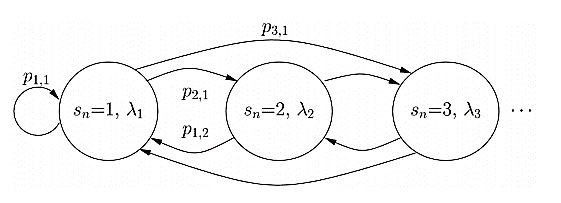
\includegraphics[scale=1]{Figures/Modelo MMPP en dispositivos MTC}
\decoRule
\caption[Modelo CMMPP en dispositivos MTC]{Modelo CMMPP: cada dispositivo MTC n está representado por una cadena de Markov con estados sn, que establecen el parámetro $\lambda$. Este parámetro es el promedio de la tasa de arribos, el cual modela el respectivo proceso de Poisson}
\label{fig:CMMPP}
\end{figure}

\end{itemize}

La principal ventaja como ya se mencionó del tráfico fuente frente al tráfico agregado es su precisión, por otra parte, la del tráfico agregado es su fácil implementación para un gran número de dispositivos. El modelo CMMPP es un intermedio entre estos dos casos, es decir mantiene la precisión del modelado de tráfico fuente mientras se mantiene la viabilidad para un gran número de máquinas. A continuación se presenta la \textit{Tabla~\ref{tab:Traficos}} con una comparativa entre los distintos modelos mencionados.\newline
\begin{table}
\caption{Comparativa entre los modelos de tráfico MTC abordados}
\label{tab:Traficos}
\centering
\begin{tabular}{|p{3in}|p{1in}|p{0.8in}|p{1in}|} \\  
\textbf{\textit{Métrica}} & \textbf{Agregado~} & \textbf{SMM} & \textbf{CMMPP} \\ \hline 
\textit{Modelado de los dispositivos} &  & \checkmark & \checkmark \\ \hline 
\textit{Modelado de dispositivos coordinados} & \checkmark &  & \checkmark \\ \hline 
\textit{Coordinación espacial y temporal} &  &  & \checkmark \\ \hline 
\textit{Modelado de los paquetes} &  & \checkmark &  \\ \hline 
\textit{Modelado de la tasa de arribo} & \checkmark & \checkmark & \checkmark \\ \hline 
\textit{Tiempo de ejecución aleatorio factible} &  & \checkmark & \checkmark \\ \hline 
\textit{Ubicación del dispositivo} &  & \checkmark & \checkmark \\ \hline 
\textit{Emparejamiento de estados} &  &  & \checkmark \\ \hline 
\textit{Complejidad (N número de dispositivos)} & O(1) & O(N) & O(N) \\  
\end{tabular}
\end{table}




Como puede observarse en la \textit{Tabla~\ref{tab:Traficos}}, las ventajas que trae consigo la utilización de un modelo de tráfico como el CMMPP son bastante convenientes para modelar el tráfico de dispositivos mIoT, pues este es capaz de simular la relación espacial y temporal que existiría entre los nodos. Si se regresa a la \textit{Tabla~\ref{tab:appssim}} en la que se presentan los servicios que se simularan, se encuentra que servicios como el monitoreo de la condición del aire en la ciudad, la detección de terremotos, la manipulación de la iluminación y demás tendrá un comportamiento similar en un espacio confinado y para poder hacer hincapié en la importancia del diseño de la red para a la hora de cumplir con la QoS esperada, es necesario que se implemente la posibilidad de recibir una gran cantidad de dispositivos en el caso de uso mMTC, los cuales estarían tratando de acceder a los recursos del sistema simultáneamente. De manera que el modelo CMMPP es el seleccionado para la simulación de este sistema complementándolo con un modelo determinístico para las aplicaciones que sólo producen tráfico periódico.\newline

Una explicación resumida del modelado  de tráfico fuente CMMPP se realiza a continuación \parencite{Gupta2018}:

\begin{enumerate}
\item  Un conjunto de \textit{k }estados se definen, cada uno asociado con una tasa de generación de paquetes ${\lambda }_k$. Un dispositivo IoT se encuentra en todo momento en algún de estos estados representados en una cadena de Markov formada por los estados antes mencionados.
\item  La transición entre los \textit{k} estados para cualquier \textit{n-ésimo}\textbf{\textit{ }}dispositivo está definida por una matriz \textit{k x k} de $P_n$ la cual es a su vez una función de dos matrices de transición $P_u$ y $P_c$ (Para comportamiento no coordinado/no sincronizado y comportamiento coordinado/sincronizado respectivamente) definidas por la red de N nodos.
\item  Un factor de correlación espacial ${\delta }_n$ se asigna a cada dispositivo \textit{n. }Esto modela qué tanto se involucra un dispositivo durante la generación de tráfico coordinado en la red y dicta efectivamente la contribución de $P_c$ en la matriz resultante de probabilidad de transición de ese dispositivo.
\item  Se define un proceso $\mathit{\Theta}\left(t\right)$ el cual controla la matriz de  transición instantánea de estado del \textit{n-ésimo}\textbf{\textit{ }}dispositivo en el instante \textit{t.}
\end{enumerate} 
% Chapter 5

\chapter{Diseño} % Main chapter title

\label{Chapter5} % Change X to a consecutive number; for referencing this chapter elsewhere, use \ref{ChapterX}


%----------------------------------------------------------------------------------------
%	SECTION 
%----------------------------------------------------------------------------------------

\section{MODELO DE SISTEMA PROPUESTO}

%----------------------------------------------------------------------------------------
%	SECTION 
%----------------------------------------------------------------------------------------

\section{RESULTADOS A OBTENER}

%----------------------------------------------------------------------------------------
%	SECTION 
%----------------------------------------------------------------------------------------

\section{METODOLOGÍA DE SIMULACIÓN}

%----------------------------------------------------------------------------------------
%	SECTION 
%----------------------------------------------------------------------------------------

\section{DEFINICIÓN DE EVENTOS}

%----------------------------------------------------------------------------------------
%	SECTION 
%----------------------------------------------------------------------------------------

\section{DIAGRAMAS DE FLUJO}
%----------------------------------------------------------------------------------------
%	SECTION 
%----------------------------------------------------------------------------------------

\section{}
%----------------------------------------------------------------------------------------
%	SECTION 
%----------------------------------------------------------------------------------------

\section{}
%----------------------------------------------------------------------------------------
%	SECTION 
%----------------------------------------------------------------------------------------

\section{}

\myworries{TODO: Agregar nuevos diagramas de acuerdo con la simulación}\newline
\myworries{TODO: Faltan palabras en ingles en italicas en este capitulo} 
% Chapter 6

\chapter{Implementación} % Main chapter title

\label{Chapter6} % Change X to a consecutive number; for referencing this chapter elsewhere, use \ref{ChapterX}


%----------------------------------------------------------------------------------------
%	SECTION 
%----------------------------------------------------------------------------------------

\section{}

%----------------------------------------------------------------------------------------
%	SECTION 
%----------------------------------------------------------------------------------------

\section{}
\myworries{AQUI VA TODO LO REFERENTE A LO QUE HEMOS HECHO EN PT2}\newline
\myworries{TODO: Faltan palabras en ingles en italicas en este capitulo} 
% Chapter 7

\chapter{Resultados} % Main chapter title

\label{Chapter7} % Change X to a consecutive number; for referencing this chapter elsewhere, use \ref{ChapterX}

El objetivo de este capítulo fue el de brindar resultados para distintos escenarios de interés, con el fin de dar comparaciones analíticas con base en la variación de los parámetros de entrada del simulador.

%----------------------------------------------------------------------------------------
%	SECTION 
%----------------------------------------------------------------------------------------

\section{Escenario I} % Simulación con un solo un TTI - FER
\subsection{Descripción del escenario}
Este escenario se concentró en obtener resultados para un solo intervalo de tiempo de transmisión (TTI), con el fin de analizar el rendimiento del modelo de despliegue de UE y el modelo de canal en conjunto con NOMA y evaluar su rendimiento.
Se simuló el rendimiento de \textit{multitone} con diferentes clases de potencia para los dispositivos MTC y con diferentes tamaños de grupos ($kmax$) pero su desempeño no resultó ser importante ya que resultaba ser similar al de singletone. Por este motivo los resultados con la propuesta multitone no se reportaron. Sin embargo, en estos resultados se implementó un modo de operación híbrido donde se adoptó un modo de operación multitone solamente cuando el número de dispositivos es menor al número de grupos (48), esto con la finalidad de no desperdiciar recursos. Y singletone en los demás casos.
También es importante señalar que la relación entre dispositivos mMTC y uRLLC es de 3 a 1.
\subsection{Parámetros de entrada}
De acuerdo con los parámetros generales del modelo de sistema [véase Tabla~\ref{tab:ParametrosGral}], los criterios considerados para este escenario fueron los siguientes:
\begin{itemize} 
	\item $k_{max} \to $ 1, 2 , 3 y 4 grupos
	\item $p_{m}^{s} \to$ 23, 20, 14 dBm
\end{itemize}

\subsection{Resultados obtenidos}
En primera instancia, en el capítulo anterior se analizó el histograma de las pérdidas de canal, del Modelo CI y también del Modelo de canal que proponen en el artículo \parencite{Shahini2019} , de acuerdo con los histogramas se tiene que el valor promedio de las perdidas [dB] en el Modelo CI son de 80.35 dBs. En contrario con las pérdidas del modelo de canal del artículo en \parencite{Shahini2019}, tienen un valor promedio de 74.67 dBs. Es decir nuestro canal tiene 3.7 (5.68 dBs) veces más perdidas en comparación del canal que se implementa en \parencite{Shahini2019}, por lo que se espera que el rendimiento sea menor, esto se puede observar en la Figura~\ref{fig:NOMA_comprobacion_CI} donde se observa que en el caso de 192 usuarios el desempeño de la simulación del artículo es aproximadamente 140 usuarios, es decir 73\% de los usuarios alcanzan su tasa objetivo. Por el contrario en la evaluación de la simulación con el modelo de canal CI en NOMA se obtiene que aproximadamente 115 usuarios alcanzan su tasa objetivo, es decir, un 60\%. Hay un rendimiento del canal CI de aproximadamente 13\% del desempeño en comparación con el canal propuesto en \parencite{Shahini2019}.\newline

Cabe destacar que en \parencite{Shahini2019}, el modelo de sistema no es implementado para una banda de frecuencias en específico, las ganancias de las subportadoras son estadísticas. En el caso de este sistema como se ocupa un modelo de canal que depende de la frecuencia, se tuvo que escoger un PRB de 180 KHz, con un conjunto de subportadoras fijadas en una banda LTE, se escogió la banda de 2GHz, esto por el hecho de que LTE se implementa en bandas de microondas. \newline

\begin{figure}[th]
    \centering
    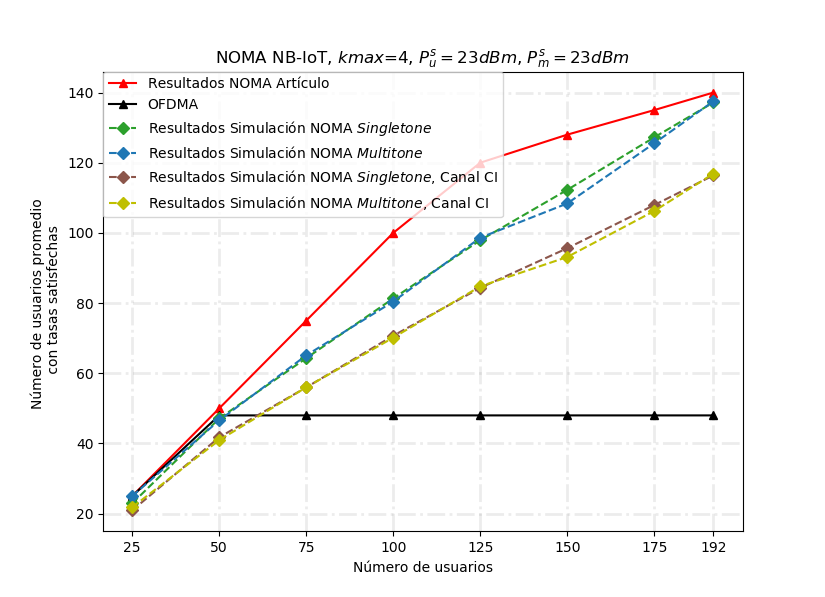
\includegraphics[scale=.7]{Figures/ResultadosNOMA/NOMA_comprobacion_CI.png}
    \decoRule
    \caption[Modelo NOMA en un TTI con modelo de canal CI]{Modelo NOMA en un TTI con modelo de canal CI}
    \label{fig:NOMA_comprobacion_CI}
\end{figure}

En la Figura~\ref{fig:NOMA_evaluacion_K_Pm_Variable_3D} se evaluó el número de usuarios que alcanzaron su tasa objetivo, se realizaron comparaciones con respecto a tres tipos de clase de potencia para los mMTC y un variable número de dispositivos por grupo (kmax).\newline

\begin{figure}[th]
    \centering
    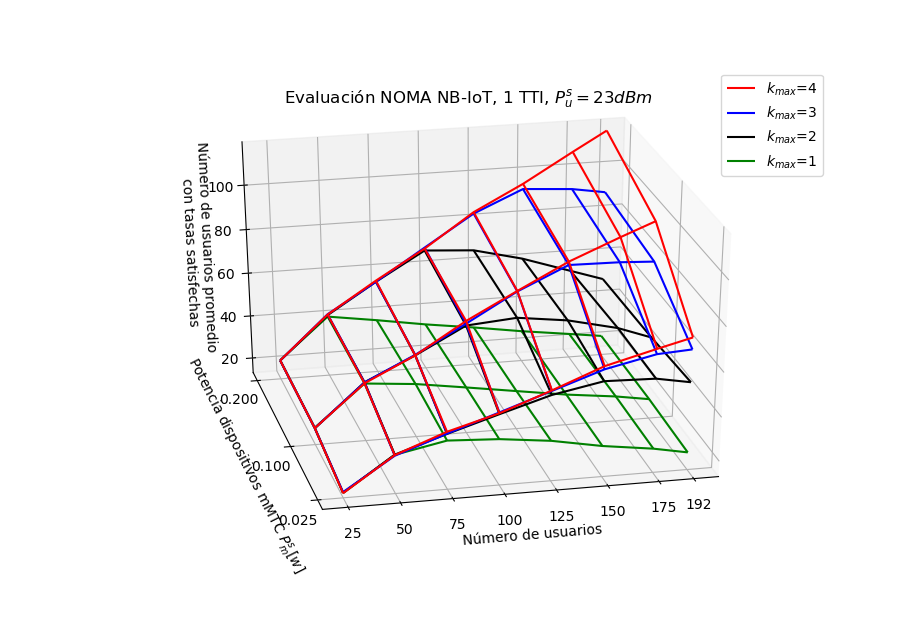
\includegraphics[scale=.7]{Figures/ResultadosNOMA/NOMA_evaluacion_K_Pm_Variable_3D.png}
    \decoRule
    \caption[Resultados generales Escenario I]{Resultados generales Escenario I}
    \label{fig:NOMA_evaluacion_K_Pm_Variable_3D}
\end{figure}

Empezando con una agrupación de 4 dispositivos, se puede observar que entre menor es la potencia de los dispositivos mMTC, el rendimiento de usuarios que alcanzan su tasa objetivo va decayendo y esto es por que al bajar su potencia los dispositivos mMTC varios de ellos comienzan a tener dificultades para alcanzar su tasa objetivo. Si se analiza el caso de 192 usuarios el desempeño con una potencia de usuarios MTC de 23dBm es de aproximadamente 115 usuarios que alcanzan su tasa objetivo, es decir, un 60\%. Y cuando la potencia de usuarios mMTC de 14dBm, 73 dispositivos alcanzan su tasa objetivo, un 38\%. Es decir el rendimiento decrece un 22\% de una potencia de 23 a 14 dBm.\newline

Con una agrupación de 3 dispositivos, vemos que el rendimiento en general decae cuando son 150 usuarios y es porque en este caso, el máximo de usuarios que pueden ser atendidos es de 144, por lo que en los casos de 175 y 192 usuarios el rendimiento va bajando esto es por la relación 3 a 1 que se propuso en los parámetros de entrada. También conforme se baja la potencia de los dispositivos mMTC, se puede ver que el rendimiento decae. Si se analiza el caso de 150 usuarios el desempeño con una potencia de usuarios MTC de 23dBm es de aproximadamente 89 usuarios que alcanzan su tasa objetivo, es decir, un 59\%. Y cuando la potencia de usuarios mMTC de 14dBm, 67 dispositivos alcanzan su tasa objetivo, un 44\%. Es decir el rendimiento decrece un 15\% de una potencia de 23 a 14 dBm.\newline

Con una agrupación de 2 dispositivos, se observa que el rendimiento en general decae cuando son 100 usuarios y es porque en este caso, el máximo de usuarios que pueden ser atendidos es de 96, por lo que en los casos mayores a 100 usuarios el rendimiento va bajando esto igualmente es por la relación 3 a 1. También, se puede ver que el rendimiento decrece cuando se baja la potencia de los dispositivos mMTC. Si se analiza el caso de 100 usuarios el desempeño con una potencia de usuarios MTC de 23dBm es de aproximadamente 53 usuarios que alcanzan su tasa objetivo, es decir, un 53\%. Y cuando la potencia de usuarios mMTC de 14dBm, 49 dispositivos alcanzan su tasa objetivo, un 49\%. Es decir el rendimiento decrece solamente 4\% de una potencia de 23 a 14 dBm.\newline

Con una agrupación de 1 dispositivo, se observa que el rendimiento en general decae cuando son 50 usuarios y es porque en este caso, el máximo de usuarios que pueden ser atendidos es de 48, por lo que en los casos mayores a 100 usuarios el rendimiento va bajando esto igualmente es por la relación 3 a 1. También conforme se baja la potencia de los dispositivos mMTC, se puede ver que el rendimiento no decae de manera significativa como lo fue en los otros casos. \newline

\break

En las siguientes figuras se evaluó la misma métrica del número de dispositivos que alcanzan su tasa objetivo pero este caso considerando cuántos de estos dispositivos son uRLLC y cuántos mMTC.\newline

\begin{figure}[th]
    \centering
    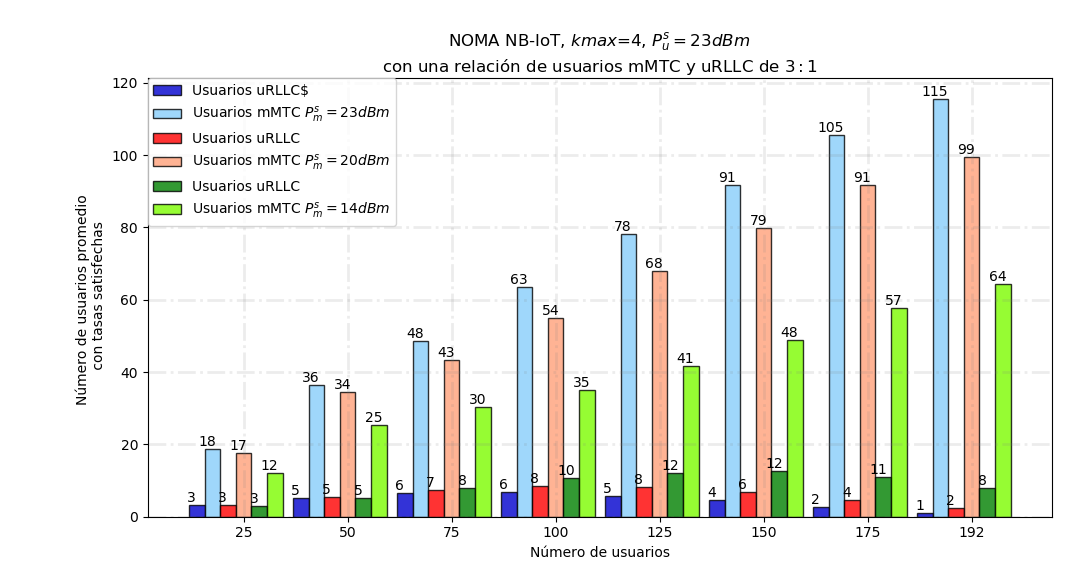
\includegraphics[scale=.65]{Figures/ResultadosNOMA/Kmax4_DiferentesPM.png}
    \decoRule
    \caption[Relación de usuarios uRLLC y mMTC que alcanzan su tasa objetivo, kmax 4]{Relación de usuarios uRLLC y mMTC que alcanzan su tasa objetivo, kmax 4}
    \label{fig:Kmax4_DiferentesPM}
\end{figure}

\begin{figure}[th]
    \centering
    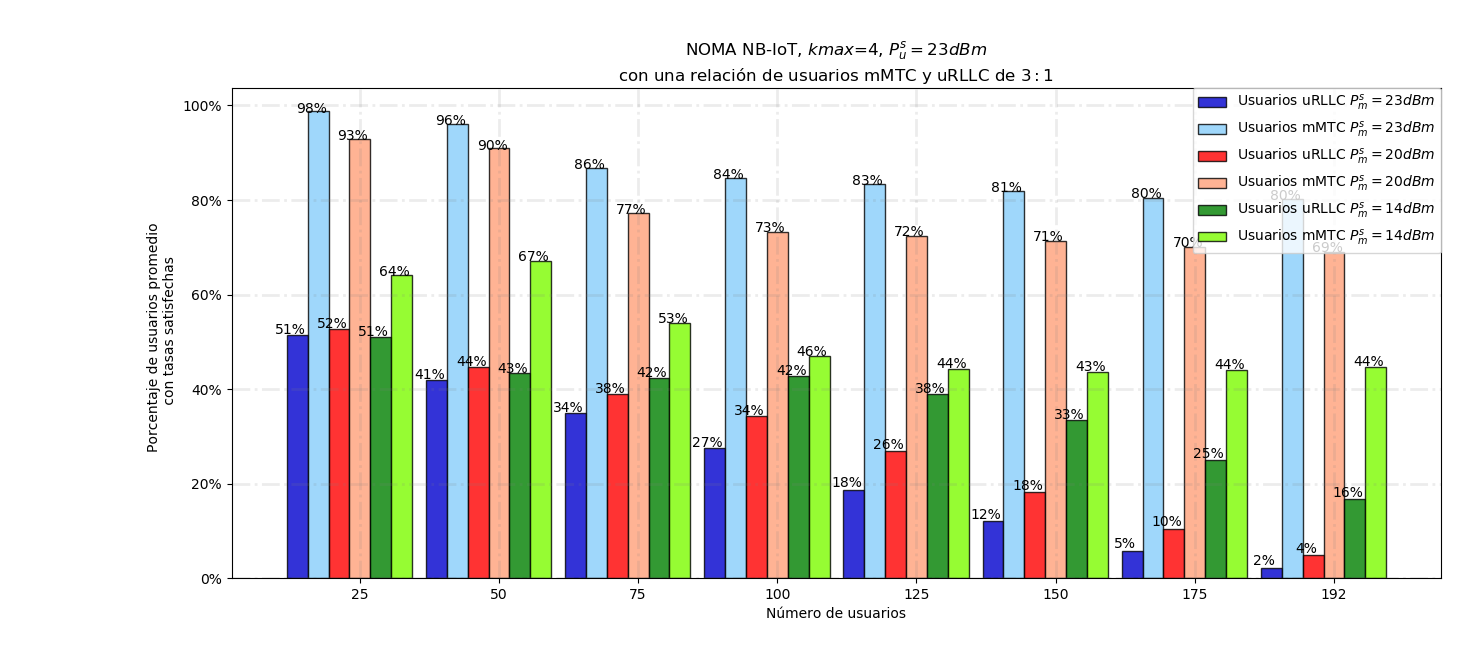
\includegraphics[scale=.65]{Figures/ResultadosNOMA/Kmax4_DiferentesPM_Porcentual.png}
    \decoRule
    \caption[Relación de usuarios uRLLC y mMTC que alcanzan su tasa objetivo $(\%)$, kmax 4]{Relación de usuarios uRLLC y mMTC que alcanzan su tasa objetivo$(\%)$, kmax 4}
    \label{fig:Kmax4_DiferentesPM_Porcentual}
\end{figure}


La Figura~\ref{fig:Kmax4_DiferentesPM} muestra la comparación del número de dispositivos mMTC y uRLLC que alcanzaron su tasa objetivo en un TTI, esto con una agrupación de 4 dispositivos (i.e. 192 dispositivos como máximo), se realizaron comparaciones con diferentes potencias de los dispositivos mMTC. Igualmente, en la Figura~\ref{fig:Kmax4_DiferentesPM_Porcentual} se representan evaluaciones acerca del número de dispositivos mMTC y uRLLC que alcanzaron su tasa objetivo, pero esta vez mostrando el porcentaje de dispositivos mMTC y uRLLC que alcanzan su tasa objetivo, de acuerdo con la relación 3 a 1 que se planteó en los parámetros de entrada.\newline

Primeramente, con una potencia de 23dBm para los dispositivos mMTC (color azul), se observa que entre mayor sea el número de dispositivos, el porcentaje de dispositivos uRLLC que alcanzan su tasa va disminuyendo, esto se puede ver más claramente en la Figura~\ref{ Kmax4_DiferentesPM_Porcentual}. Por ejemplo., cuando son 25 dispositivos el porcentaje de uRLLC y mMTC es de 51\% y 98\%, respectivamente, y cuando el número de dispositivos aumenta a 192, el porcentaje de uRLLC y mMTC es de 2\% y 80\%, respectivamente, (esto es con base en la relación 3 a 1). Como se observa la relación entre uRLLC y mMTC que alcanzan su tasa es injusta, esto debido a que al transmitir con la misma potencia todos los dispositivos, la contribución de interferencia de los dispositivos mMTC (en rangos altos) para los uRLLC, es bastante alta, impidiendo que los uRLLC no alcancen sus tasas objetivo.\newline

En los casos en donde la potencia de los dispositivos mMTC es menor a la de los uRLLC, se observa una mejor proporción entre los dispositivos. Por ejemplo, con una potencia de 14dBm para los dispositivos mMTC (color verde) el porcentaje de dispositivos uRLLC y mMTC es de 51\% y 64\%, respectivamente, y cuando el número de dispositivos aumenta a 192, el porcentaje de dispositivos uRLLC y mMTC es de 16\% y 44\%, respectivamente, (esto es con base en la relación 3 a 1). Como se observa la relación de uRLLC y mMTC que alcanzan su tasa es mas equitativa comparado con el análisis de potencia de los dispositivos mMTC con 23 dBm. \newline

\break

\begin{figure}[th]
    \centering
    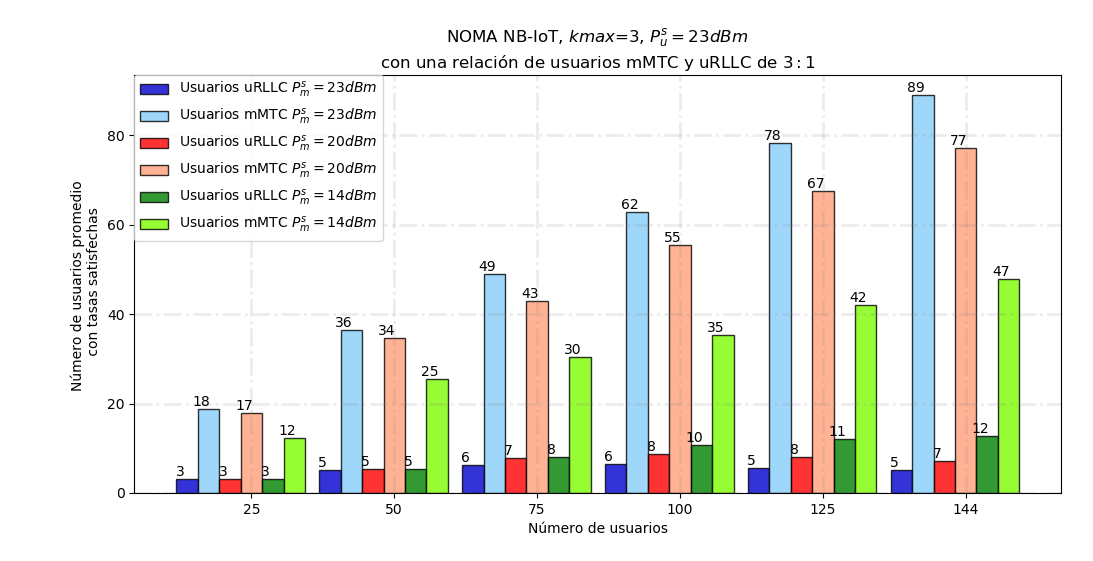
\includegraphics[scale=.65]{Figures/ResultadosNOMA/Kmax3_DiferentesPM.png}
    \decoRule
    \caption[Relación de usuarios uRLLC y mMTC que alcanzan su tasa objetivo, kmax 3]{Relación de usuarios uRLLC y mMTC que alcanzan su tasa objetivo, kmax 3}
    \label{fig:Kmax3_DiferentesPM}
\end{figure}

\begin{figure}[th]
    \centering
    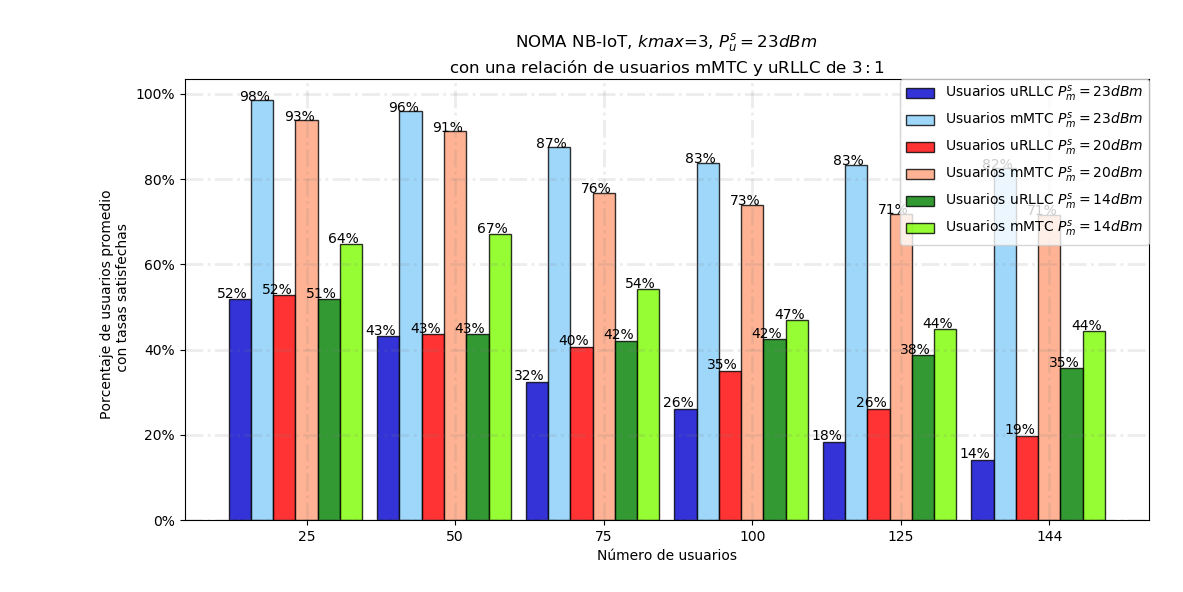
\includegraphics[scale=.65]{Figures/ResultadosNOMA/Kmax3_DiferentesPM_Porcentual.png}
    \decoRule
    \caption[Relación de usuarios uRLLC y mMTC que alcanzan su tasa objetivo $(\%)$, kmax 3]{Relación de usuarios uRLLC y mMTC que alcanzan su tasa objetivo$(\%)$, kmax 3}
    \label{fig:Kmax3_DiferentesPM_Porcentual}
\end{figure}

Las Figuras~\ref{fig:Kmax3_DiferentesPM} y ~\ref{fig:Kmax3_DiferentesPM_Porcentual} representan la relación entre el número de dispositivos mMTC y uRLLC que alcanzaron su tasa objetivo en un TTI, esto con una agrupación de 3 dispositivos (i.e. 144 dispositivos como máximo), se realizaron comparaciones con diferentes potencias de los dispositivos mMTC.\newline

Primeramente, con una potencia de 23dBm para los dispositivos mMTC (color azul), se observa que entre mayor sea el número de dispositivos, la relación de dispositivos uRLLC y mMTC que alcanzan su tasa se hace más desproporcional, esto se puede ver más claramente en la Figura~\ref{fig:Kmax3_DiferentesPM_Porcentual}. Por ejemplo, cuando son 25 dispositivos el porcentaje de dispositivos uRLLC y mMTC es de 52\% y 98\%, respectivamente, y cuando el número de dispositivos aumenta a 144, el porcentaje de dispositivos uRLLC y mMTC es de 14\% y 82\%, respectivamente, (esto es con base en la relación 3 a 1). La relación de uRLLC y mMTC que alcanzan su tasa sigue siendo injusta pero no en gran cantidad comparado con agrupaciones de 4 dispositivos, esto es porque son menos los dispositivos agrupados.\newline

En los casos en donde la potencia de los dispositivos mMTC es menor a la de los uRLLC, se observó, que se obtiene una mejor proporción entre los dispositivos. Por ejemplo, con una potencia de 14dBm para los dispositivos mMTC (color verde) el porcentaje de dispositivos uRLLC y mMTC es de 51\% y 64\%, respectivamente, y cuando el número de dispositivos aumenta a 144, el porcentaje de dispositivos uRLLC y mMTC es de 35\% y 44\%, respectivamente, (esto es con base en la relación 3 a 1). \newline

\break

\begin{figure}[th]
    \centering
    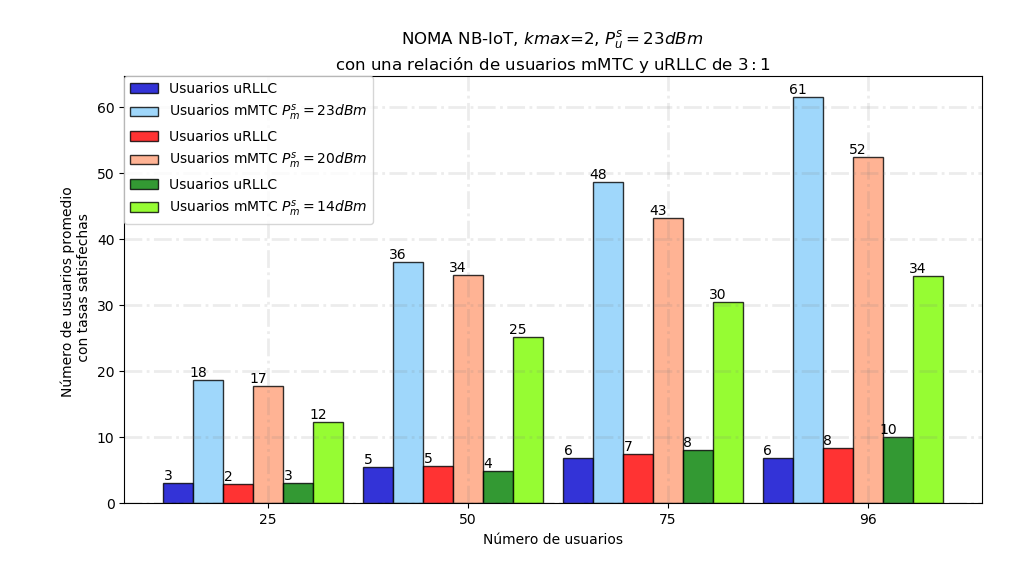
\includegraphics[scale=.6]{Figures/ResultadosNOMA/Kmax2_DiferentesPM.png}
    \decoRule
    \caption[Relación de usuarios uRLLC y mMTC que alcanzan su tasa objetivo, kmax 2]{Relación de usuarios uRLLC y mMTC que alcanzan su tasa objetivo, kmax 2}
    \label{fig:Kmax2_DiferentesPM}
\end{figure}

\begin{figure}[th]
    \centering
    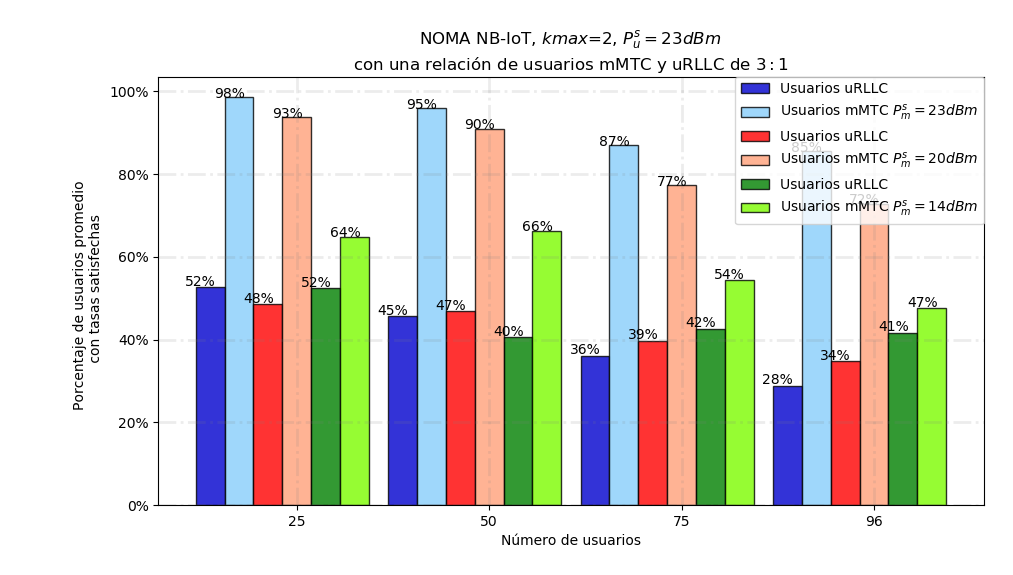
\includegraphics[scale=.6]{Figures/ResultadosNOMA/Kmax2_DiferentesPM_Porcentual.png}
    \decoRule
    \caption[Relación de usuarios uRLLC y mMTC que alcanzan su tasa objetivo $(\%)$, kmax 2]{Relación de usuarios uRLLC y mMTC que alcanzan su tasa objetivo$(\%)$, kmax 2}
    \label{fig:Kmax2_DiferentesPM_Porcentual}
\end{figure}

Las Figuras~\ref{fig:Kmax2_DiferentesPM} y ~\ref{fig:Kmax2_DiferentesPM_Porcentual} representan la relación entre el número de dispositivos mMTC y uRLLC que alcanzaron su tasa objetivo en un TTI, esto con una agrupación de 2 dispositivos (i.e. 96 dispositivos como máximo), se realizaron comparaciones con diferentes potencias de los dispositivos mMTC.\newline

Primeramente, con una potencia de 23dBm para los dispositivos mMTC (color azul), se observa que entre mayor sea el número de dispositivos, la relación de dispositivos uRLLC y mMTC que alcanzan su tasa se hace desproporcional, esto se puede ver más claramente en la Figura~\ref{fig:Kmax2_DiferentesPM_Porcentual}. Por ejemplo, cuando son 25 dispositivos, los porcentajes de dispositivos uRLLC y mMTC es de 52\% y 98\%, respectivamente, y cuando el número de dispositivos aumenta a 96 dispositivos, el porcentaje de dispositivos uRLLC y mMTC es de 28\% y 85\%, respectivamente, (esto es con base en la relación 3 a 1). \newline

En los casos en donde la potencia de los dispositivos mMTC es menor a la de los uRLLC, se observó la relación entre los dispositivos alcanzan una mejor proporción. Por ejemplo, Con una potencia de 14dBm para los dispositivos mMTC (color verde) el porcentaje de dispositivos uRLLC y mMTC es de 52\% y 64\%, respectivamente, y cuando el número de dispositivos aumenta a 144 dispositivos, el porcentaje de dispositivos uRLLC y mMTC es de 41\% y 47\%, respectivamente, (esto es con base en la relación 3 a 1). \newline


Para finalizar esta sección, se pudo observar que de la Figura~\ref{fig:NOMA_evaluacion_K_Pm_Variable_3D}, que entre menor sea la potencia de transmisión de los dispositivos mMTC, el número de dispositivos que alcanzan su tasa objetivo disminuirá, pero al hacer el análisis de las gráficas de la relación de dispositivos uRLLC y mMTC, se concluye, que aunque disminuyen los dispositivos que alcanzan su tasa, mejora equitativamente la proporción entre los dispositivos uRLLC y mMTC que logran su tasa objetivo.

\break
%----------------------------------------------------------------------------------------
%	SECTION 
%----------------------------------------------------------------------------------------

\section{Escenario II} % Simulación completa con tráfico - 

Este segundo escenario pone a prueba la capacidad que tiene el programa principal \textbf{Simulador de modelos de tráfico para nodos IoT en una red celular de 5G}, de generar resultados que permitan comparar el efecto que tiene establecer distintos parámetros de la red en el \textit{throughput} del sistema y en el porcentaje de dispositivos que cumplen su tasa deseada. \newline

\subsection{Descripción del escenario}

En este este escenario se consideraron únicamente los dispoitivos de tipo URLLC y los llamados Otros dispositivos mMTC, esto para cumplir fácilmente con la relación de 3 a 1 entre ambos tipos de dispositivos. Entonces en el programa \textbf{Generador de tráfico IoT} se generó tráfico dentro de una célula de radio igual a 200 metros. La distribución de usuarios se hizo con la opción PPP y se establecieron las intensidades de la siguiente forma: La intensidad de los dispositivos mMTC se fijo en 0.3 $dispositivos/m^2$ y la de los dispositivos URLLC se fijo en 0.1 $dispositivos/m^2$. La relación de dispositivos se eligió 3 a 1 para después fijar las tasas de nacimientos de paquetes y de alarmas idénticas en ambos tipos de servicios y garantizar que el tráfico ofrecido al sistema conserve esa relación. La tasa de nacimiento de paquetes es $\lambda_{normal} = 0.0167 paquetes/seg.$ y la de nacimiento de alarmas es $\lambda_{alarma} = 0.1 alarmas/seg.$ para ambos tipos de dispositivos. Finalmente, las características en las que se transmiten las alarmas son compartidas también entre ambos dispositivos: $velocidad_{alarma} = 500 m/s$ y para el modelo de propagación espacial se usó el modelo de ventana de coseno alzado con $d_{th}=200$ y $d_{th}=100$. \newline

De manera que virtualmente, ambos tipos los dispositivos generan tráfico a la misma tasa, pero al haber 3 veces más dispositivos mMTC, en los algoritmos NOMA se conservará en promedio esta relación.

El tráfico generado por el \textbf{Generador de tráfico IoT} correspondió a 10 segundos y la iteración seleccionada para ser evaluada por el simulador de eventos discretos contenía 2 alarmas, una para cada tipo de dispositivo, lo que es el promedio esperado, dado que $\lambda_{alarma} = 0.1 alarmas/seg.$. Se seleccionó esta iteración por ser una buena representación de los parámetros ingresados. Finalmente se inició la simulación con 48 dispositivos ya utilizando el canal, 26 dispositivos mMTC y 12 URLLC, esto para que el sistema se encontrara ya en un equilibrio de operación.

\subsection{Parámetros de entrada}

La instancia de tráfico utilizada como entrada del simulador de eventos discretos, comprendía $37541$ dispositivos mMTC y $12611$ dispositivos URLLC. El tiempo de la simulación se fijo en $10$ segundos y la potencia máxima de transmisión se fijó como $23dBm$ para los dispositivos URLLC. Finalmente se usó $d0=1m$, $PLE=2.0$ y el bloque de frecuencias que inicia en $2Ghz$. 

Se corrieron 12 rutinas en las que se variaron los valores de $k$ desde $1$ hasta $4$ y la potencia máxima de transmisión de los dispoitivos mMTC tomó valores de 23, 20 y 14 dBm.

\subsection{Resultados obtenidos}
%                                           PONER ESTO EN TABLA

Los resultados obtenidos en este escenario II se encuentran registrados en las siguientes tablas y corresponden siempre a evaluación de 12 puntos, generados apartir de las 12 combinaciones posibles de tamaño de cluster y potencia máxima de transmisión de los dispositivos mMTC. \newline

%                                           HACER ANALISIS DE GRAFICAS
\begin{figure}[th]
    \centering
    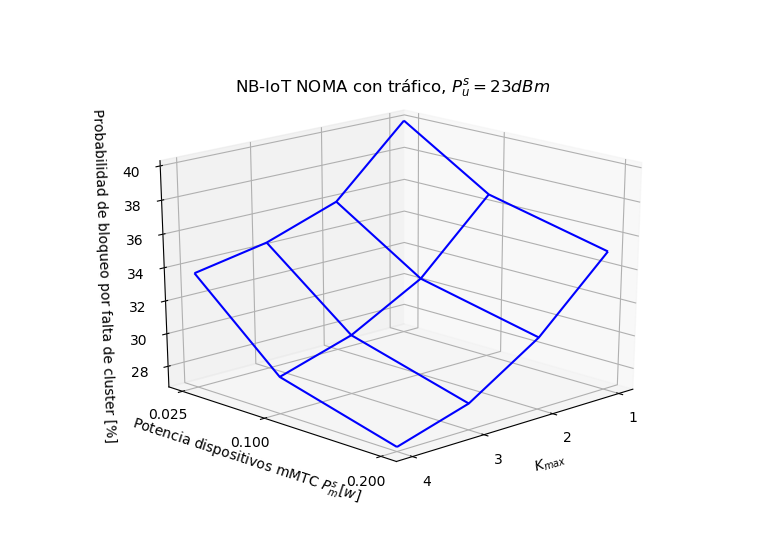
\includegraphics[scale=0.9]{Figures/ResultadosTrafico/Figure_1.png}
    \decoRule
    \caption[Probabilidad de bloque por falta de recursos]{[Probabilidad de bloque por falta de recursos}
    \label{fig:bloqueocluster}
\end{figure}

La Figura~\ref{fig:bloqueocluster}, muestra la probabilidad de bloqueo por falta de cluster. Se trata de la probabilidad que tiene cada paquete generado de ser bloqueado debido a que el dispositivo IoT no consiguió entrar a un cluster (es decir no se le asignaron recursos). Se puede notar que esta probabilidad decrece cuando se agregan más rangos a cada cluster y cuando aumenta $P_{m}^{s}$. De manera que la menor probabilidad de bloque por falta de un cluster o recursos asignados es cuando $k_{max}=4$ y $P_{m}^{s}=0.200 W$. \newline


\begin{figure}[th]
    \centering
    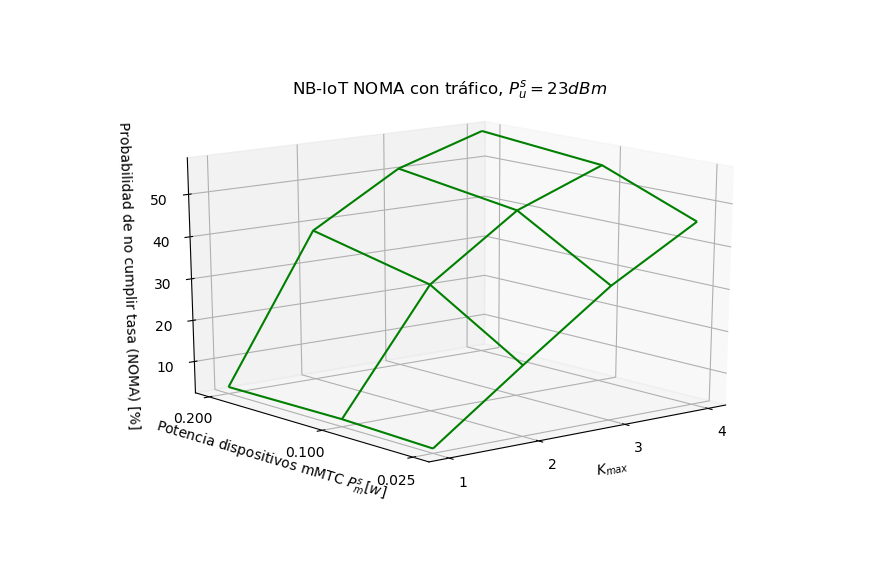
\includegraphics[scale=0.9]{Figures/ResultadosTrafico/Figure_2.png}
    \decoRule
    \caption[Probabilidad de no cumplir la tasa objetivo]{Probabilidad de no cumplir la tasa objetivo}
    \label{fig:tasa}
\end{figure}

La Figura~\ref{fig:tasa}, muestra la probabilidad que tiene cada dispositivo de no cumplir con su tasa objetivo. Esta se calcula al final de la transmisión de cada paquete, utilizando el tamaño del paquete y el tiempo que tomó transmitirlo. En la figura se puede apreciar que la menor probabilidad de que un paquete no cumpla con su tasa objetivo es para los clusters de tamaño uno, es decir cuando no se realiza NOMA. Al mismo tiempo, cuando la potencia máxima de los dispoitivos mMTC toma el valor mínimo, la probabilidad de no cumplir con la tasa objetivo parece aumentar, sin embargo se necesitarían de más corridas para concluir sobre esto. Pero pareciera que la potencia no es suficiente, cuando el tamaño de los cluster aumenta, para que todos los dispositivos mMTC cumplan con su tasa objetivo. \newline


\begin{figure}[th]
    \centering
    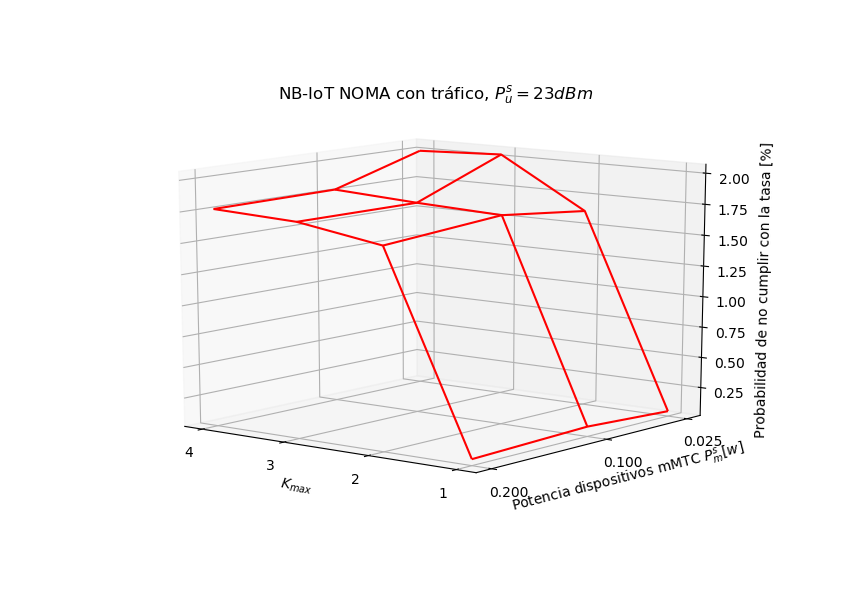
\includegraphics[scale=0.9]{Figures/ResultadosTrafico/Figure_3.png}
    \decoRule
    \caption[Probabilidad de no cumplir la tasa objetivo entre procesos NOMA]{Probabilidad de no cumplir la tasa objetivo durante un proceso NOMA}
    \label{fig:tasaNOMA}
\end{figure}

La Figura~\ref{fig:tasaNOMA}, muestra la probabilidad de que un dispositivo no consiga transmitir a su tasa objetivo al terminar un proceso NOMA y hasta el inicio del siguiente. Es importante recordar que un proceso NOMA se realiza cada que nace y cada que se termina de transmitir un paquete, de manera que muchos procesos NOMA tendrán lugar durante la transmisión completa de un sólo paquete. La tasa mostrada en la gráfica anterior podría considerarse la tasa efectiva, mientras que esta muestra la tasa en pequeños intervalos de tiempo. En la figura se puede apreciar que el orden de las probabilidades es mucho mayor que aquel en la Figura~\ref{fig:tasa}, lo que deja ver que aunque los dispositivos transmitan paquetes por debajo de su tasa objetivo durante muchos intervalos de tiempo, finalmente logran cumplir con su tasa objetivo en un porcentaje mucho mayor. Un comportamiento esperado, que se podría inferir también de esta figura es que al aumentar el tamaño de los clusters, menos dispositivos alcanzarán su tasa objetivo en estos pequeños intervalos de tiempo. Sin embargo no es tan fácil concluir esto de la tasa efectiva (La mostrada en la Figura~\ref{fig:tasa}).\newline

\begin{figure}[th]
    \centering
    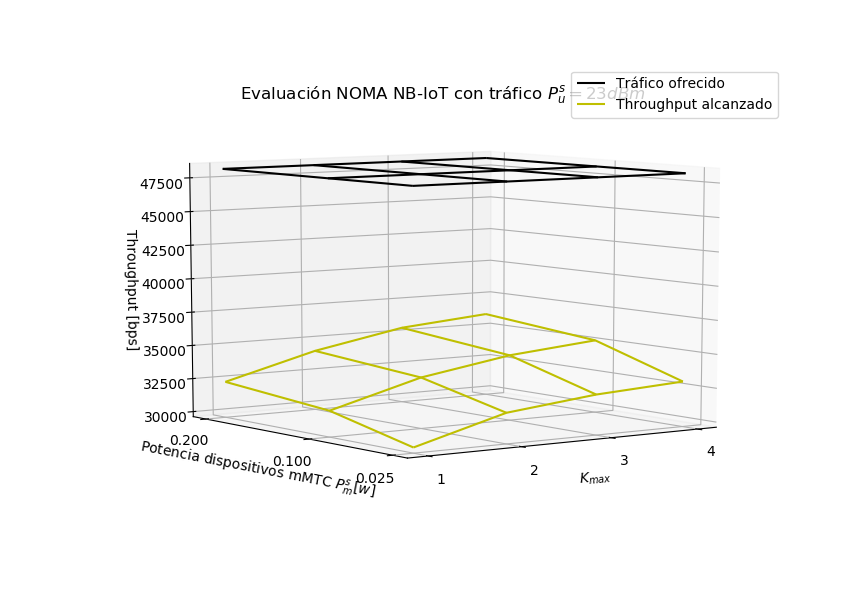
\includegraphics[scale=0.9]{Figures/ResultadosTrafico/Figure_4.png}
    \decoRule
    \caption[Throughput]{Throughput}
    \label{fig:throughput2}
\end{figure}

Finalmente, la Figura~\ref{fig:throughput2}, muestra el \textit{throughput} logrado en cada una de las 12 corridas de la simulación. Se puede ver que se logra un aumento en éste cuando se admiten más dispositivos en cada cluster y cuando aumenta la potencia de máxima de transmisión de los dispositivos mMTC.\newline 

Con ayuda de estas gráficas se puede comenzar a inferir que la mejor opción para aumentar el \textit{throughput} y reducir la probabilidad de bloqueo por falta de recursos es seleccionando $k_{max}=4$ y $P_{m}^{s}=0.200W$, a cambio claro de aumentar la probabilidad de no cumplir con las tasas objetivo de cada dispositivo. Sin embargo más corridas serían necesarias para hacer conclusiones, pero se puede apreciar que los resultados arrojados por el simulador son capaces de mostrar los efectos que tiene cambiar dos variables sobre el comportamiento del sistema.\newline 
% Chapter 8

\chapter{Conclusiones} % Main chapter title

\label{Chapter8} % Change X to a consecutive number; for referencing this chapter elsewhere, use \ref{ChapterX}

En este capítulo se concluye el presente proyecto, compilando una discusión y un análisis crítico de los resultados en general, presentando las posibilidades de evolución futura de las comunicaciones móviles, así como las propuestas de trabajo académico futuro a mediano plazo.

%----------------------------------------------------------------------------------------
%	SECTION 
%----------------------------------------------------------------------------------------

\section{Generales}

%----------------------------------------------------------------------------------------
%	SECTION 
%----------------------------------------------------------------------------------------

\section{Específicas}

 

%----------------------------------------------------------------------------------------
%	THESIS CONTENT - APPENDICES
%----------------------------------------------------------------------------------------

\appendix % Cue to tell LaTeX that the following "chapters" are Appendices

% Include the appendices of the thesis as separate files from the Appendices folder
% Uncomment the lines as you write the Appendices

% Appendix A

\chapter{Distribuciones estadísticas en Telecomunicaciones} % Main appendix title

\label{AppendixA} % For referencing this appendix elsewhere, use \ref{AppendixA}

El objetivo de este apéndice fue revisar las distribuciones de probabilidad mas utilizadas en los sistemas de comunicaciones móviles para caracterizar los fenómenos más importantes en este ámbito, después se describió la implementación y puesta a prueba de la generación de las variables aleatorias utilizadas en el simulador, esto con el fin de brindar fiabilidad en los resultados obtenidos.\newline

%----------------------------------------------------------------------------------------
%	SECTION 1
%----------------------------------------------------------------------------------------

El uso de modelos estadísticos es importante para describir diferentes fenomenos en el campo de las telecomunicaciones\parencite{Correia2018}:
\begin{itemize}
    \item Llamadas telefónicas y conexiones de datos
    \item Influencia del usuario en el rendimiento de la red
    \item Propagación no guiada en ambientes aleatorios
    \item Movilidad del usuario
\end{itemize}

Comúnmente se utilizan las siguientes distribuciones de probabilidad en telecomunicaciones \parencite{Correia2018}:

\begin{enumerate}
    \item Distribución Uniforme: Es usada para describir la fase de una señal. También, se ha utilizado para simular el despliegue de BSs \parencite{TurjmanSmallCells}.
    \item Distribución Normal (Gaussiana): Es usada para describir fluctuaciones alrededor de un valor medio, p.ej. \textit{shadowing}. Esta distribución no puede ser usada para describir entidades que no pueden ser negativas.
    \item Distribución Log-Normal: Es usada para describir entidades como la potencia de una señal, amplitudes, principalmente el desvanecimiento lento.
    \item Distribución Rayleigh: Es usada para describir el desvanecimiento rápido-intenso.
    \item Distribución Susuki: Describe conjuntamente el desvanecimiento lento y rápido.
    \item Distribución Rice: Es usada para describir el desvanecimiento rápido - no-intenso.
    \item Distribución Exponencial: Es ampliamente usada para describir la duración de diferentes fenómenos, principalmente asociados con el desvanecimiento de señales y las llamadas telefónicas.
    \item Distribución de Bernoulli: Es usada para describir la ocupación de canales de telecomunicaciones.
    \item Distribución binomial: Es usada para describir llamadas telefónicas.
\end{enumerate}

\section{Generación de números aleatorios}

La distribución uniforme (también llamada distribución rectangular) es una familia de curvas de dos parámetros que es notable porque tiene una función de distribución de probabilidad constante (PDF) entre sus dos parámetros delimitadores. La distribución uniforme se utiliza en técnicas de generación de números aleatorios, como el método de inversión \parencite{ UniformMatlab}.\newline

Se puede usar la distribución uniforme estándar para generar números aleatorios para cualquier otra distribución continua mediante el método de inversión. El método de inversión se basa en el principio de que las funciones de distribución acumulativa continua (CDFs) varían uniformemente durante el intervalo abierto $(0, 1)$ . Si $u$ es un número aleatorio uniforme en (0, 1) , entonces $x = F^{ -1} ( u )$ genera un número aleatorio $x$ a partir de la distribución continua con la CDF especificada $F$ \parencite{UniformMatlab}.\newline

En teoría de la probabilidad y estadística, hay varias relaciones entre las distribuciones de probabilidad. Estas relaciones se pueden clasificar en los siguientes grupos \parencite{univariateDist}:
\begin{itemize}
    \item Una distribución es un caso especial de otra con un espacio de parámetros más amplio.
    \item Transformaciones (función de una variable aleatoria).
    \item Combinaciones (función de varias variables).
    \item Relaciones de aproximación (límite).
    \item Relaciones compuestas (útiles para la inferencia bayesiana [\textit{Bayesian inference}]).
\end{itemize}

\begin{figure}[th]
    \centering
    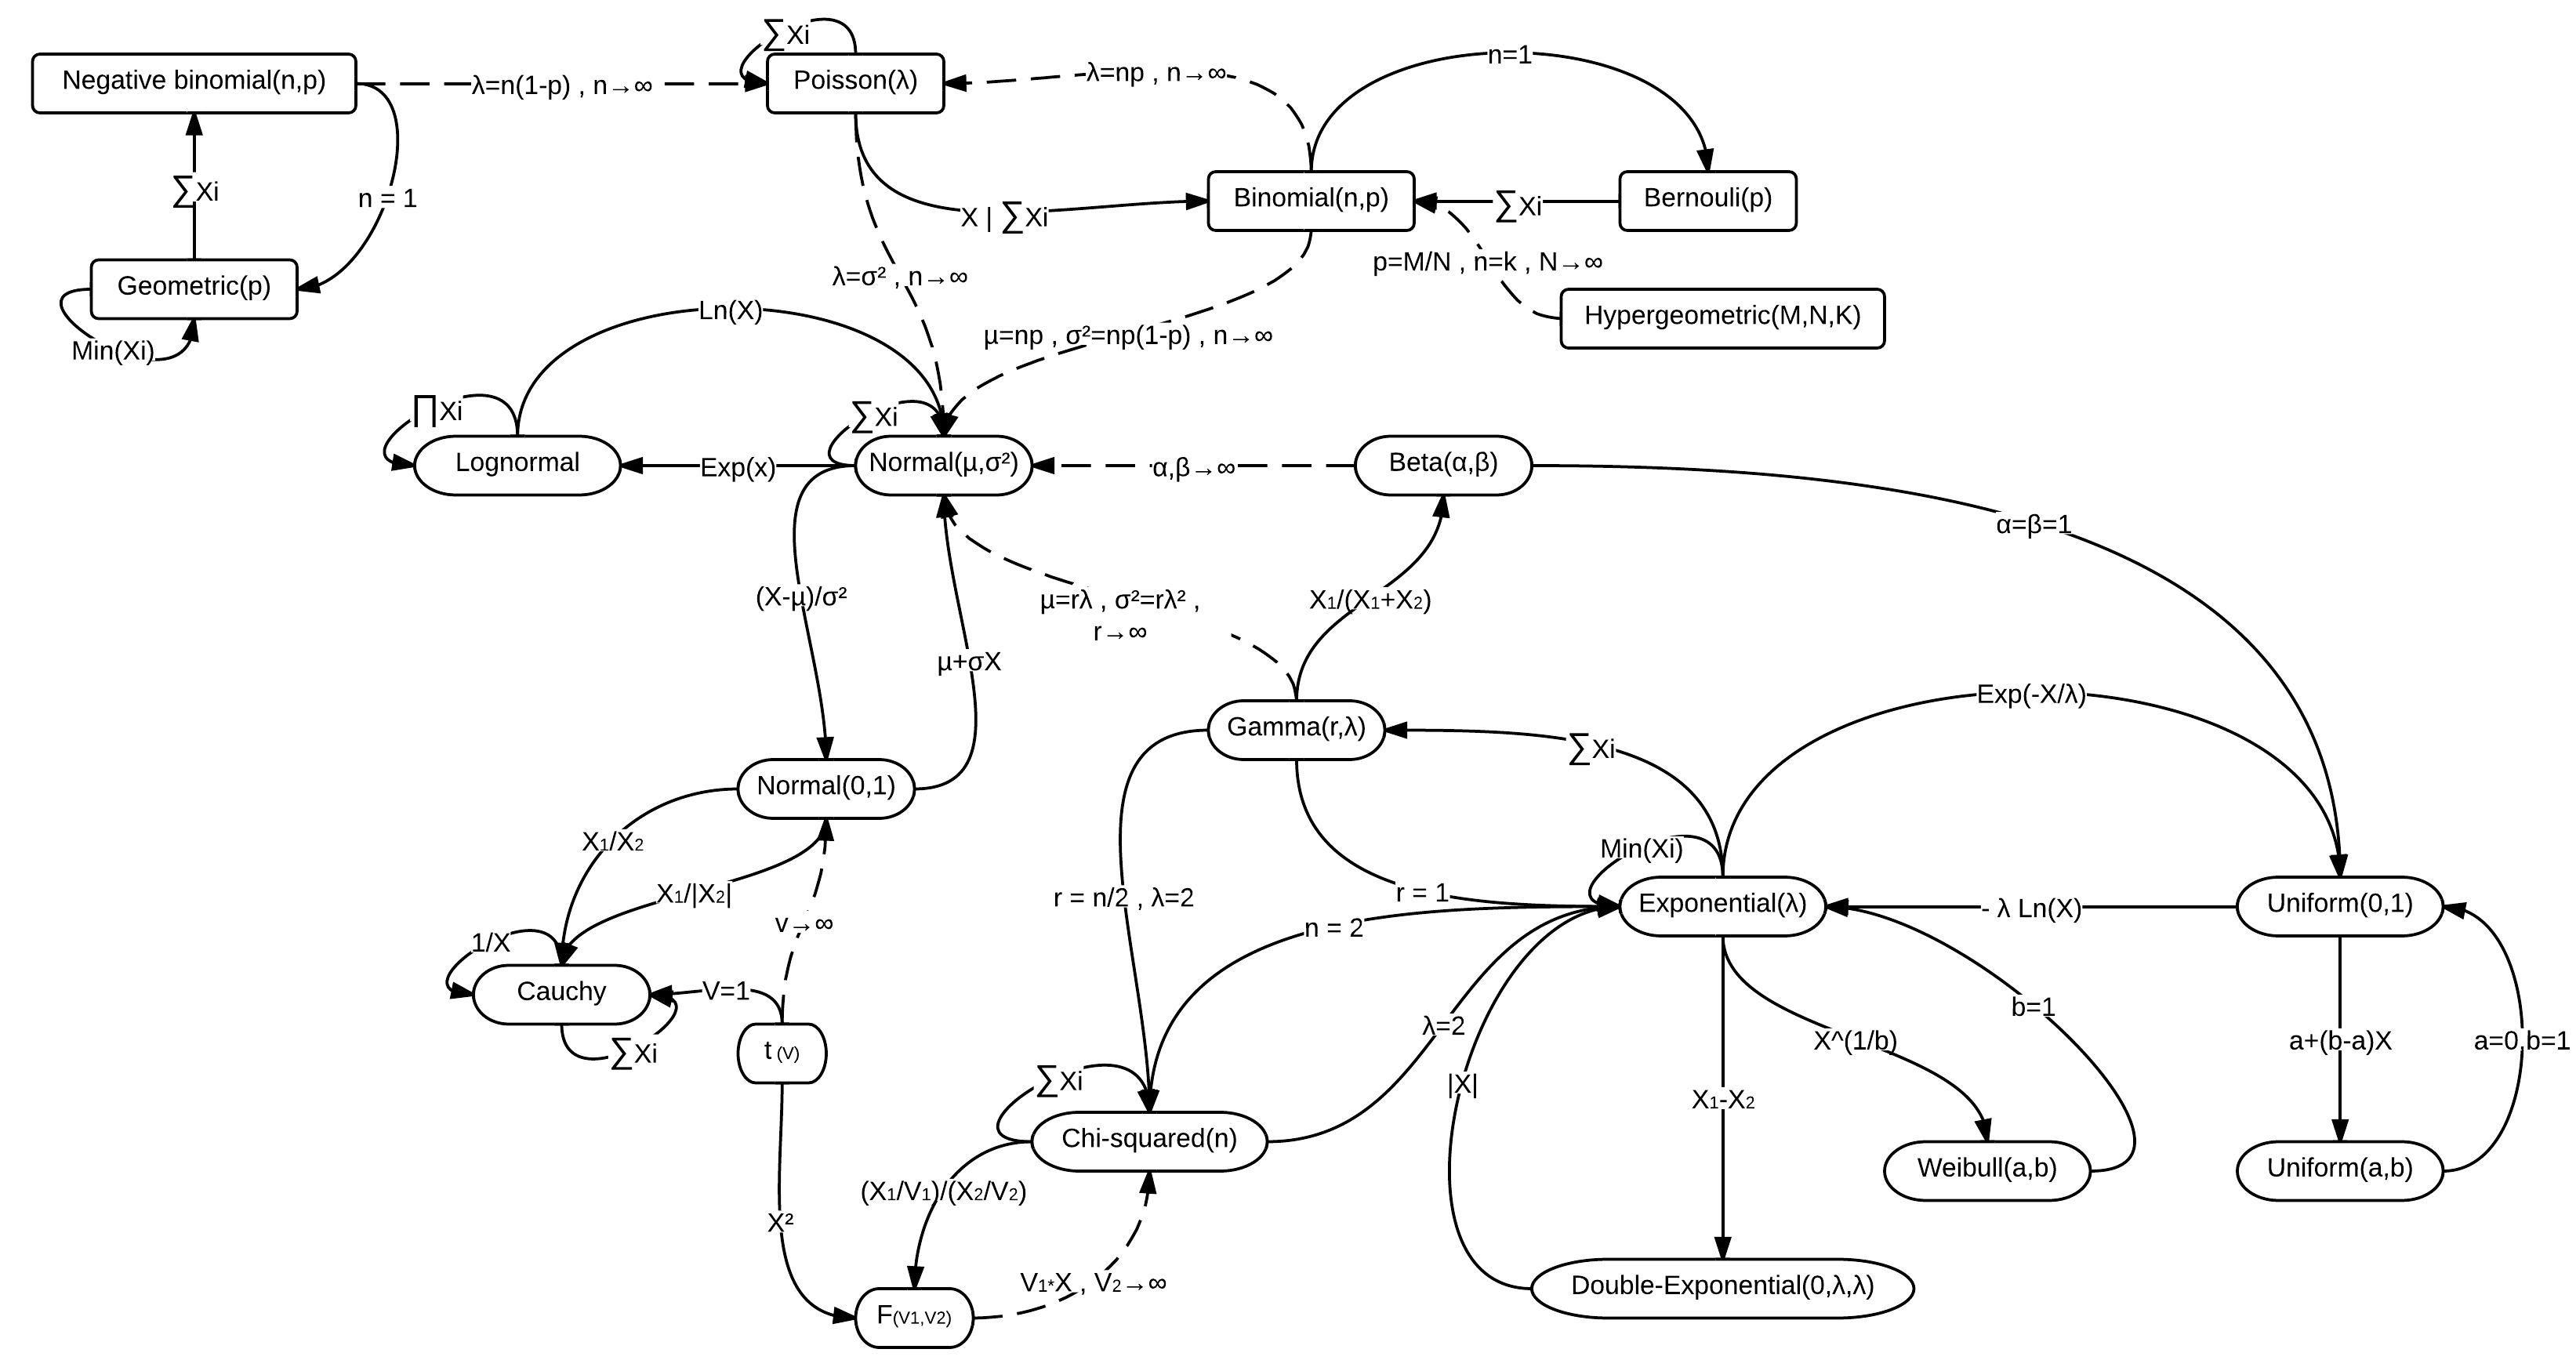
\includegraphics[scale=0.63]{Figures/RelacionesProbabilidad}
    \decoRule
    \caption[Relaciones entre algunas de las distribuciones de probabilidad univariadas]{Las relaciones entre algunas de las distribuciones de probabilidad univariadas se ilustran con líneas conectadas, las líneas discontinuas significan relación aproximada. [Fuente: \parencite{univariateDist}]}
    \label{fig:relacionesDistribuciones}
\end{figure}

\break

\section{Generación de distribuciones estadísticas para el simulador}

\subsection{Generación de variable aleatoria tipo \textit{Poisson}}
Como se revisó en la sección~\ref{generarGeoEstocastica}, uno de los requisitos para generar una geometría estocástica es que el número de puntos en el plano sea Poisson, es por esto que en esta sección se comprobó la generación de la variable aleatoria Poisson en Python usando la libreria \textit{scipy}.\newline

Para esto, se realizaron $10000$ generaciones de numeros siguiendo una distribución de Poisson con tasa $\lambda = 20$, se obtuvo el histograma de todos los números generados y se comparó con su función de masa de probabilidad (PMF).\newline

Se observa que la distribución del histograma sigue a la función masa de probabilidad de Poisson [\textit{véase Figura~\ref{fig:generacionPoisson}}], por lo que se valida la generación de números Poisson en Python.\newline

\begin{figure}[th]
    \centering
    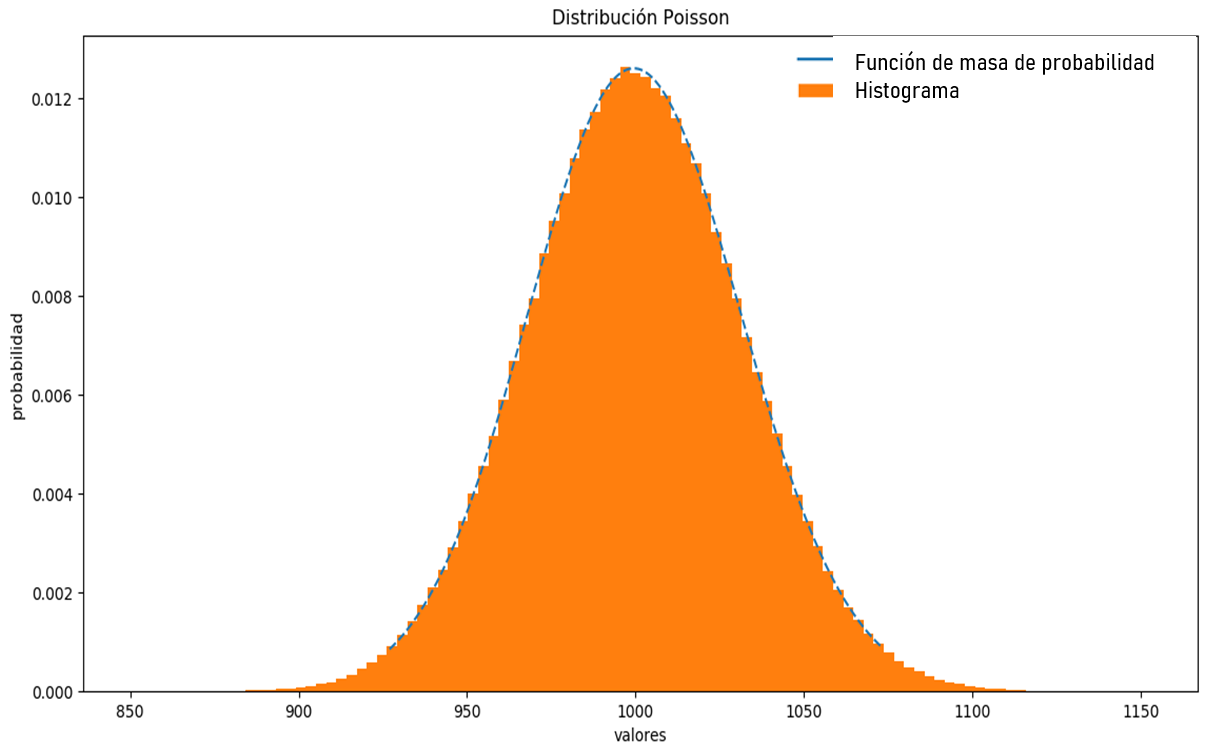
\includegraphics[scale=.5]{Figures/PoissonDistribution}
    \decoRule
    \caption[Gráfica comparación PMF e histograma de distribución Poisson en Python]{Gráfica comparación PMF e histograma de distribución Poisson en Python}
    \label{fig:generacionPoisson}
\end{figure}
\break

\subsection{Generación de variables aleatorias tipo \textit{Exponencial} y \textit{Rayleigh}}

Como se revisó en la sección~\ref{DesvRayleigC2}, cuando el desvanecimiento es de tipo Rayleigh, la magnitud o amplitud de la señal es Rayleigh y la potencia es exponencial. En esta sección, se comprobó la generación de estas variables aleatorias en Python usando la libreria \textit{random}.\newline

Se realizaron $10000$ generaciones de numeros siguiendo una distribución Exponencial negativa con media $\mu =1$, se obtuvo el histograma de todos los números generados y se comparó con su función de densidad de probabilidad (PDF).\newline

De la misma manera con la otra distribución, se realizaron $10000$ generaciones de numeros siguiendo una distribución Rayleigh con desviación estándar $\sigma = 1$, se obtuvo el histograma de todos los números generados y se comparó con su función de densidad de probabilidad (PDF).\newline

Se observa que la distribuciones de los histogramas siguen a su respectiva función densidad de probabilidad (PDF) [\textit{véanse Figuras~\ref{fig:generacionExpon} y \ref{fig:generacionRay} }], por lo que se valida la generación de números Exponenciales y Rayleigh en Python.\newline

\begin{figure}[th]
    \centering
    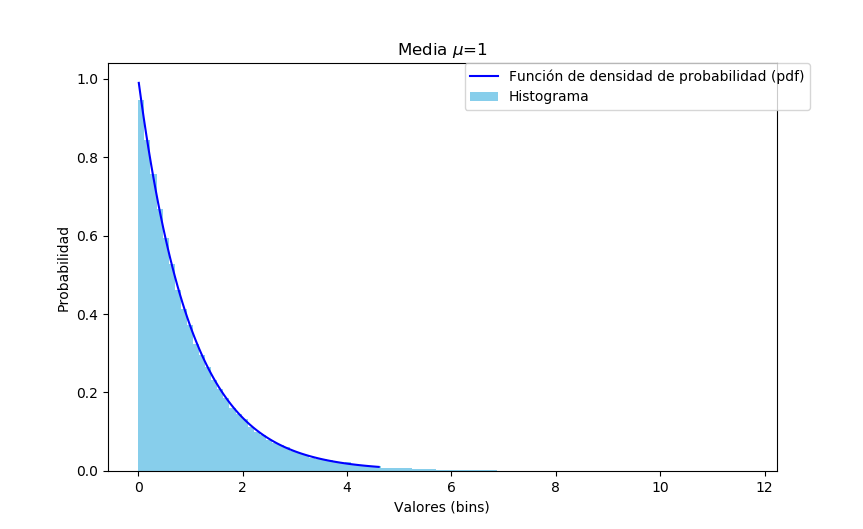
\includegraphics[scale=.6]{Figures/ExponentialDisitribution.png}
    \decoRule
    \caption[Gráfica comparación PDF e histograma de distribución Exponencial en Python]{Gráfica comparación PDF e histograma de distribución Exponencial en Python}
    \label{fig:generacionExpon}
\end{figure}

\begin{figure}[th]
    \centering
    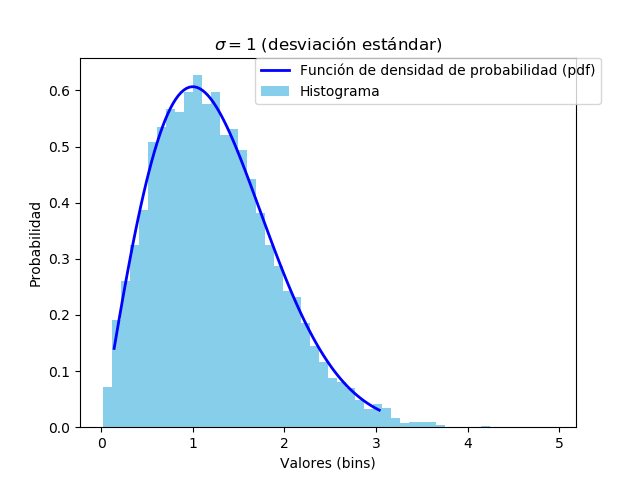
\includegraphics[scale=.7]{Figures/RayleighDistribution.png}
    \decoRule
    \caption[Gráfica comparación PDF e histograma de distribución Rayleigh en Python]{Gráfica comparación PDF e histograma de distribución Rayleigh en Python}
    \label{fig:generacionRay}
\end{figure}
\break

\subsection{Generación de variable aleatoria tipo \textit{Pareto}}

Como se revisó en la sección~\ref{Informesperiodicos}, la longitud de paquetes en la transmisión periodica siguió una distribución de Pareto con parámetro alfa = 2.5 y tamaño mínimo de carga útil de la aplicación = 20 bytes con un corte a 200 bytes.\newline

La distribución de Pareto a veces se conoce como el Principio de Pareto o la regla '80 –20 ', en este caso la regla establece que el 80\% de los tamaños de paquete que se formarán, los producirán solo el 20\% de los dispositivos del sistema y viceversa.\newline

La distribución de Pareto se puede replicar en Python usando el módulo Scipy.stats o NumPy. El módulo Scipy.stats abarca varias distribuciones de probabilidad y una biblioteca cada vez mayor de funciones estadísticas. Se comprobó la generación de esta variable aleatoria en Python usando la libreria \textit{scipy}.\newline

Se realizaron $100000$ generaciones de numeros siguiendo una distribución areto con parámetro alfa  $\alpha =2.5$ acotada entre 20 y 200, se obtuvo el histograma de todos los números generados y se comparó con su función de densidad de probabilidad (PDF).\newline

Se observa que la distribución del histograma sigue a la función densidad de probabilidad Pareto [\textit{véase Figura~\ref{fig:generacionPareto}}], por lo que se valida la generación de números Pareto en Python.\newline

\begin{figure}[th]
    \centering
    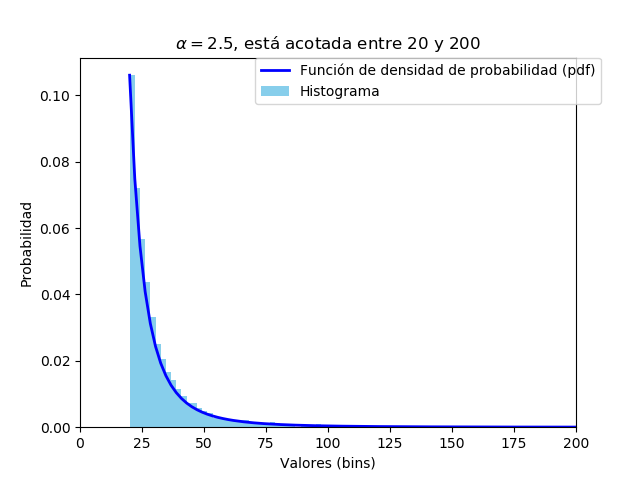
\includegraphics[scale=.7]{Figures/ParetoDIstribution}
    \decoRule
    \caption[Gráfica comparación PDF e histograma de distribución Pareto en Python]{Gráfica comparación PDF e histograma de distribución Pareto en Python}
    \label{fig:generacionPareto}
\end{figure}


%% Appendix B

\chapter{Simulación - Geometría celular hexagonal} % Main appendix title

\label{AppendixB} % For referencing this appendix elsewhere, use \ref{AppendixA}

\section{Generación de despliegue Uniforme de usuarios}

\section{Análisis de Geometría Celular un una celda}
%\include{Appendices/AppendixC}

%----------------------------------------------------------------------------------------
%	BIBLIOGRAPHY
%----------------------------------------------------------------------------------------
\printbibliography[heading=bibintoc]

%----------------------------------------------------------------------------------------

\end{document}  
